\documentclass[../document.tex]{subfiles}
\begin{document}
\section{Implementation}
In this section we reveal the details about the implementation tools and choices. We will start from the employed software, then we will describe each step in the dataset generation and finishing by illustrate the utilized estimators.
\subsection{Tools}
We quickly list the most important tools and libraries adopted in this project:
\begin{itemize}
    \item ROS Melodic
    \item Numpy
    \item Matplotlib
    \item Pandas
    \item OpenCV
    \item PyTorch
    \item FastAI
    \item imgaug
    \item Blender
\end{itemize}
The framework was entirely developed on Ubuntu 18.10 with Python 3.6.

\subsubsection{ROS Melodic}
The Robot Operating System (ROS) \cite{ROS} is a flexible framework for writing robot software. It is \emph{de facto} the industry and research standard framework for robotics due to its simple yet effective interface that facilitates the task of creating a robust and complex robot behavior regardless of the platforms. ROS works by establishing a peer-to-peer connection where each \emph{node} is to communicate between the others by exposing sockets endpoints, called \emph{topics}, to stream data or send \emph{messages}. 

Each \emph{node} can subscribe to a \emph{topic} to receive or publish new messages. In our case, \emph{Krock} exposes different topics on which we can subscribe in order to get real-time information about the state of the robot.
Unfortunately, ROS does not natively support Python3, so we had to compile it by hand. Because it was a difficult and time-consuming operation, we decided to share the ready-to-go binaries as a \href{https://hub.docker.com/r/zuppif/ros-melodic-python3/}{docker image}. 
% \footnote{\href{https://hub.docker.com/r/zuppif/ros-melodic-python3/}} 


\subsubsection{Numpy}
\href{https://www.numpy.org/}{Numpy} is a fundamental package for any scientific use. It allows to express efficiently any matrix operation using its broadcasting functions. Numpy is used across the whole pipeline to manipulate matrices.

\subsubsection{Matplotlib}
Almost all the plots in this report were created by \href{https://matplotlib.org/}{Matplotlib}, is a Python 2D plotting library. It provides a similar functional interface to MATLAB and a deep ability to customize every region of the figure. All 
It is worth citing \emph{seaborn} a data visualization library that we inglobate in our work-flow to create the heatmaps. It is based on Matplotlib and it provides an high-level interface.
\subsubsection{Pandas}
To process the data from the simulations we rely on \href{https://pandas.pydata.org/}{Pandas}, a Python library providing fast, flexible, and expressive data structures in a tabular form. Pandas is well suited for many different kinds of data such as handle tabular data with heterogeneously-typed columns, similar to SQL table or Excel spreadsheet, time series and matrices. We take advantages of the relationa data structure to perform custom manipulation on the rows by removing the outliears and computing the advancement.

Generally, pandas does not scale well and it is mostly used to handle small dataset while relegating \"big data\" to other frameworks such as Spark or Hadoop. We used Pandas to store the results from the simulator and inside a Thread Queue to parse each \emph{.csv} file efficiently. 

\subsubsection{OpenCV}
Open Source Computer Vision Library, \href{https://opencv.org/}{OpenCV}, is an open source computer vision library with a rich collection of highly optimized algorithms. It includes classic and state-of-the-art computer vision and machine learning methods applied in a wide array of tasks, such as object detection and face recognition. We adopt this library to handle image data, mostly to pre and post-process the heightmaps and the patches.
\subsubsection{PyTorch}
\href{https://pytorch.org/}{PyTorch} is a Python open source deep learning framework. It allows Tensor computation (like NumPy) with strong GPU acceleration and Deep neural networks built on a tape-based auto grad system. Due to its Python-first philosophy, it is easy to use, expressive and predictable it is widely used amoung researches and enthusiast. Moreover, its main advantages over other mainstream frameworks such as TensorFlow \cite{tensorflow} are a cleaner API structure, better debugging, code shareability and an enormous number of high-quality third-party packages.

\subsubsection{FastAI}
\href{https://course.fast.ai/}{FastAI} is library based on PyTorch that simplifies fast and accurate neural nets training using modern best practices. It provides a high-level API to train, evaluate and test deep learning models on any type of dataset. We used it to train, test, and evaluate our models.

\subsubsection{imgaug}
\href{https://imgaug.readthedocs.io/en/latest/}{Image augmentation} (imgaug) is a python library to perform image augmenting operations on images. It provides a variety of methodologies, such as affine transformations, perspective transformations, contrast changes and Gaussian noise, to build sophisticated pipelines. It supports images,  heatmaps, segmentation maps, masks, key points/landmarks, bounding boxes, polygons, and line strings. We used it to augment the heightmap, details are in \hyperref[sec: data-aug]{section \ref{sec: data-aug}}

\subsubsection{Blender}
\href{https://www.blender.org/}{Blender} is the free and open source 3D creation suite. It supports the entirety of the 3D pipeline modeling, rigging, animation, simulation, rendering, compositing and motion tracking, even video editing and game creation. We used Blender to render some of the 3D terrain utilized to evaluate the trained model.

\todo[inline]{I switched to mayavi}
\subsection{Data Gathering}
In this section we describe how we generate the synthetic maps, how we the robot interacts with them and all the postprocessing needed to create the final dataset.
\subsubsection{Heightmap generation}
To collect the data throught simulation we first need to generate meaningful terrain to be explored by the robot. Each map are stored as heightmap, a 2D array, an image, where each pixel's value represents the terrain height. The following figure shows an heightmap representing a real world \emph{Quarry} and the relative terrain.
\begin{figure}[H]
    \centering
        \begin{subfigure}[b]{0.45\textwidth}
            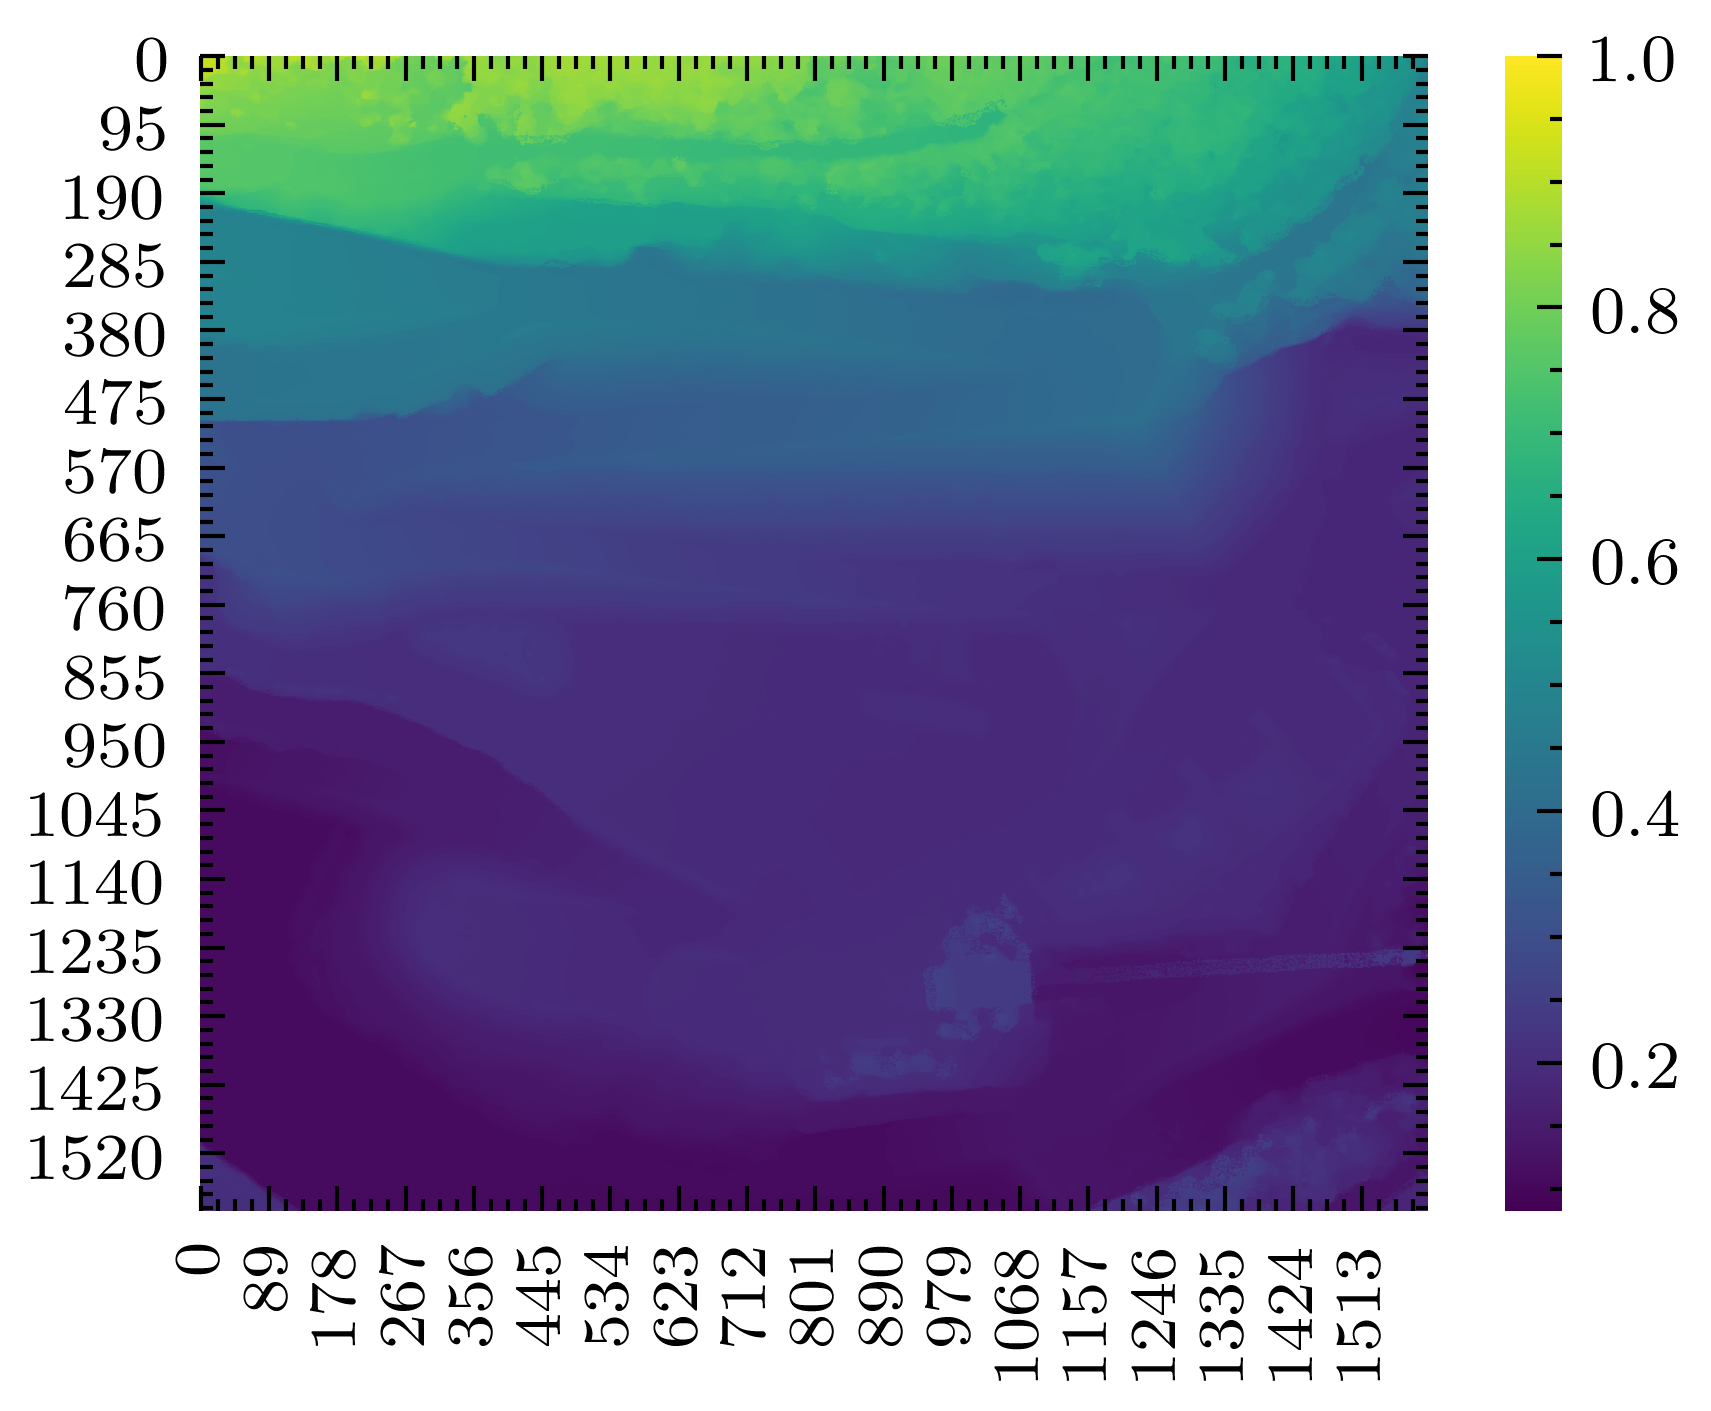
\includegraphics[width=\textwidth]{../img/hm/querry-big-10.png}
            \caption{An heightmap representing a \emph{Quarry}.}
        \end{subfigure}
        \begin{subfigure}[b]{0.45\linewidth}
            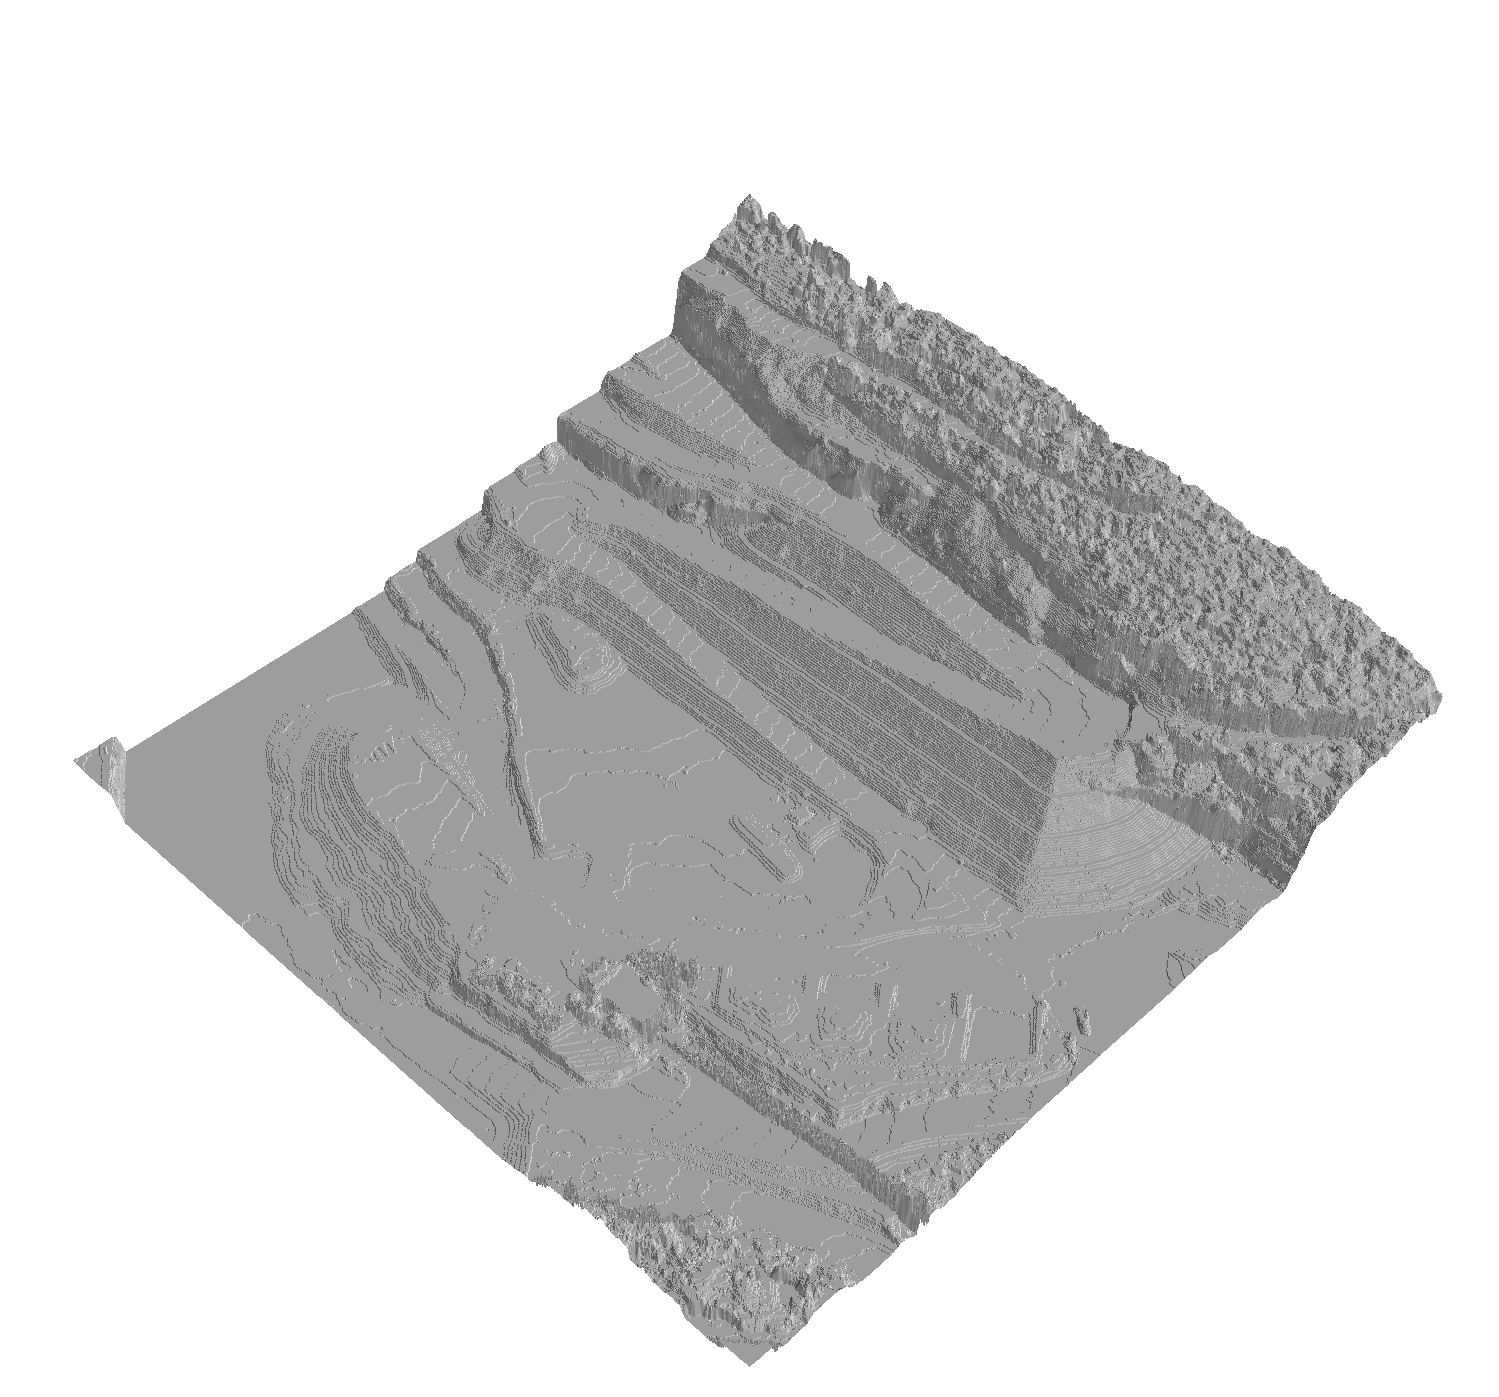
\includegraphics[width=\textwidth]{../img/hm3d/querry-big-10.png}
            \caption{3D rendered}
            \end{subfigure}    
    \caption{This image shows an heightmap and the 3D render of a Quarry.}
    \end{figure}
We created thirty maps of $513\times513$ pixel with a resolution of $0.02cm/pixel$ in order to represent a $10\times10m$ terrain. To generate them with 2D simplex noise \cite{simplex}, a variant of Perlin noise \cite{perlin}, a widely used technique in the terrain generation litterature. We divide the maps into five main categories of terrains: $bumps$, $rails$, $steps$, $slopes$/$ramps$ and $holes$. For some map we add three different rocky texture to create more complicated situations, all the maps configuration are shown in table \ref{table: maps}.

\paragraph{Bumps:} 
We genered four different maps with increasing bumps' height using simplex noise with features size $\in[200,100,50,25 ]$. 
\begin{figure}[H]
    \centering
        \begin{subfigure}[b]{0.32\textwidth}
            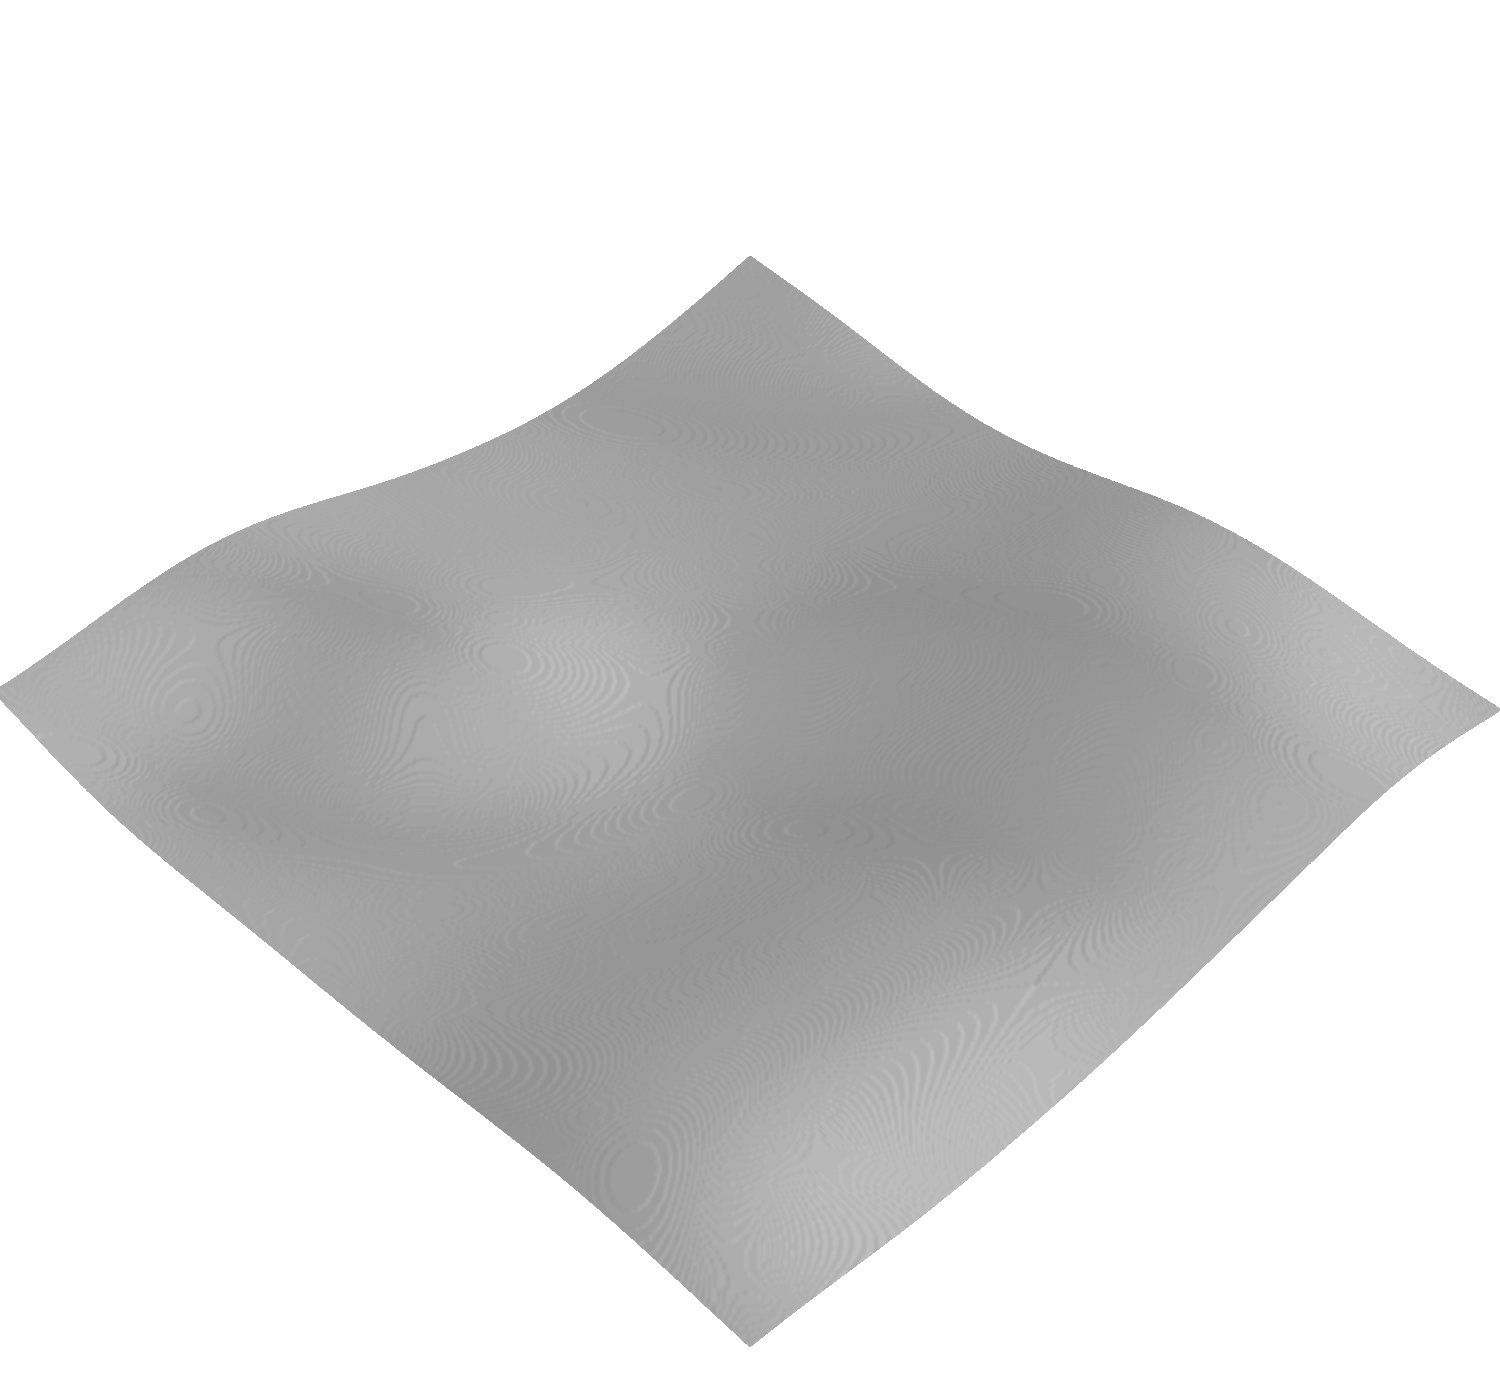
\includegraphics[width=\textwidth]{../img/hm3d/bumps0.png}
            \caption{\emph{bumps0}}
        \end{subfigure}
        \begin{subfigure}[b]{0.32\linewidth}
            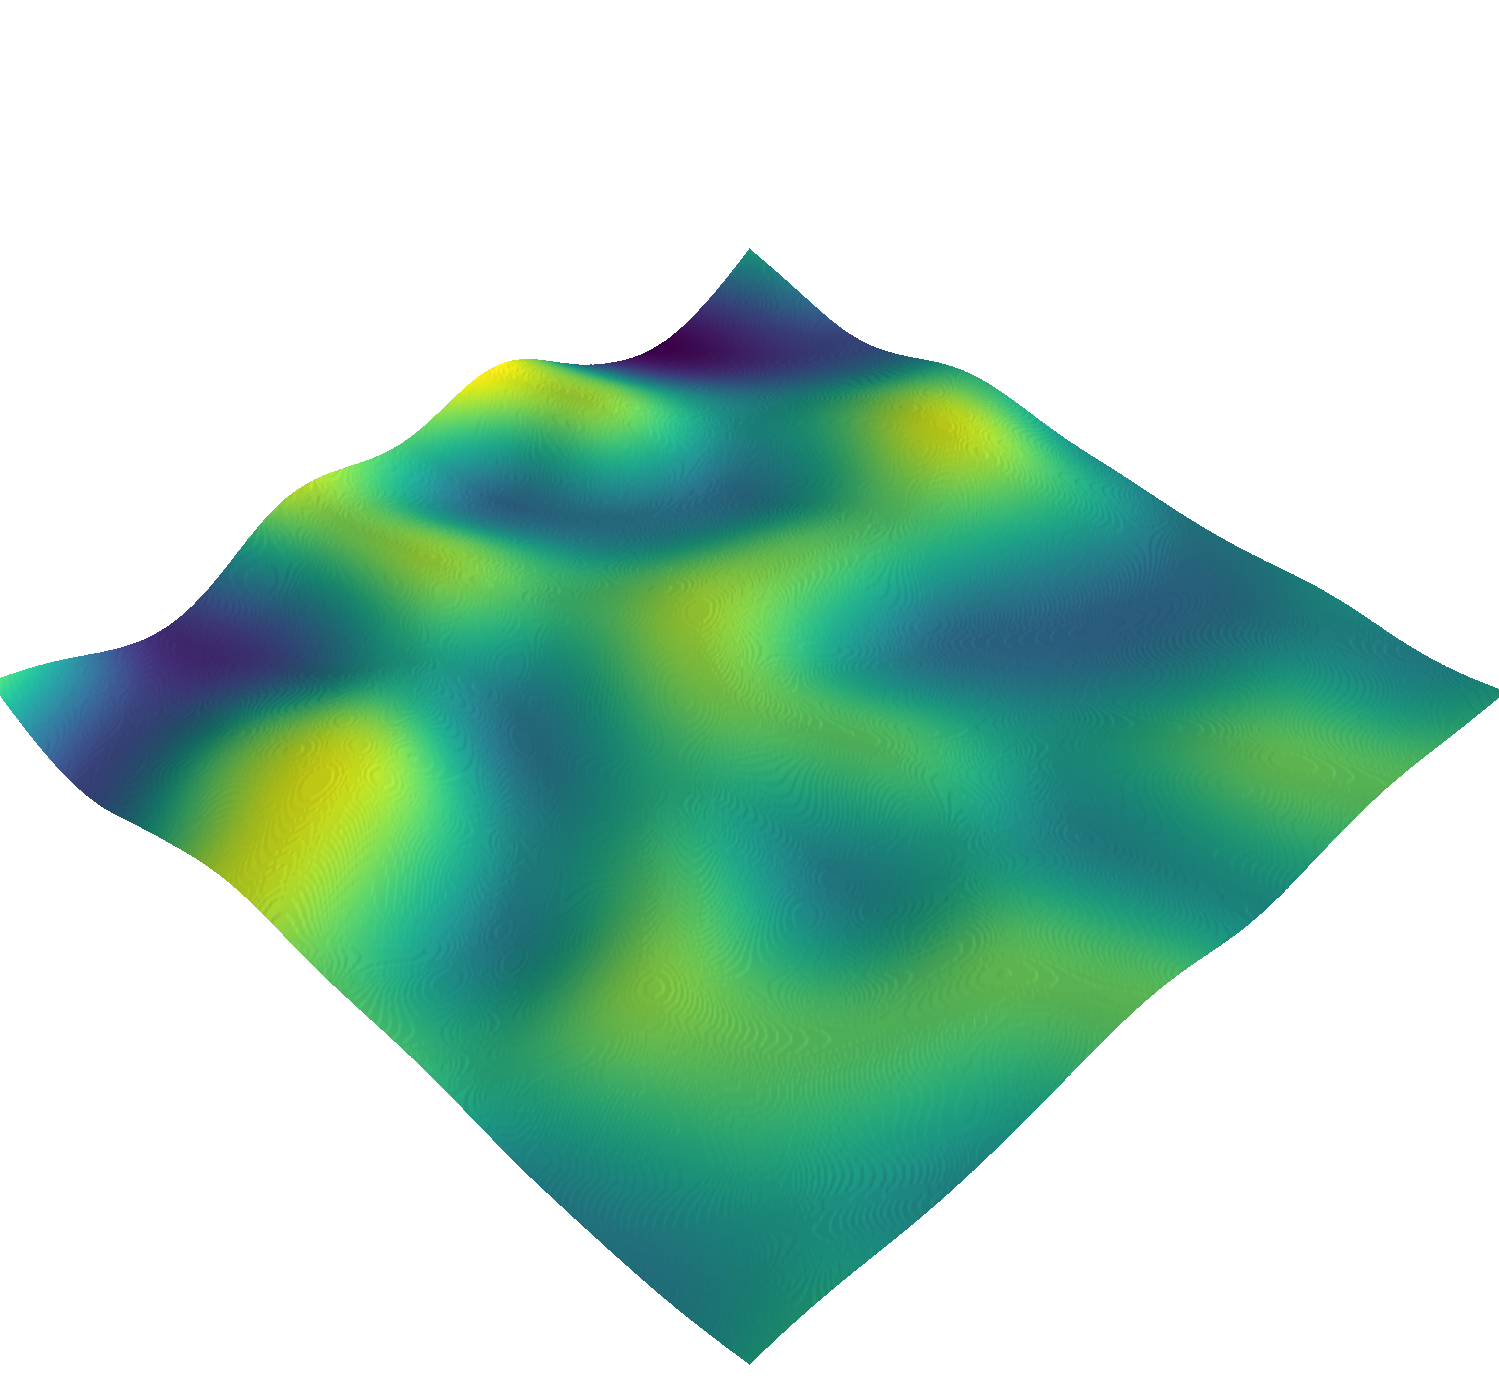
\includegraphics[width=\textwidth]{../img/hm3d/bumps1.png}
            \caption{\emph{bumps1}}
            \end{subfigure}    
          \begin{subfigure}[b]{0.32\textwidth}
            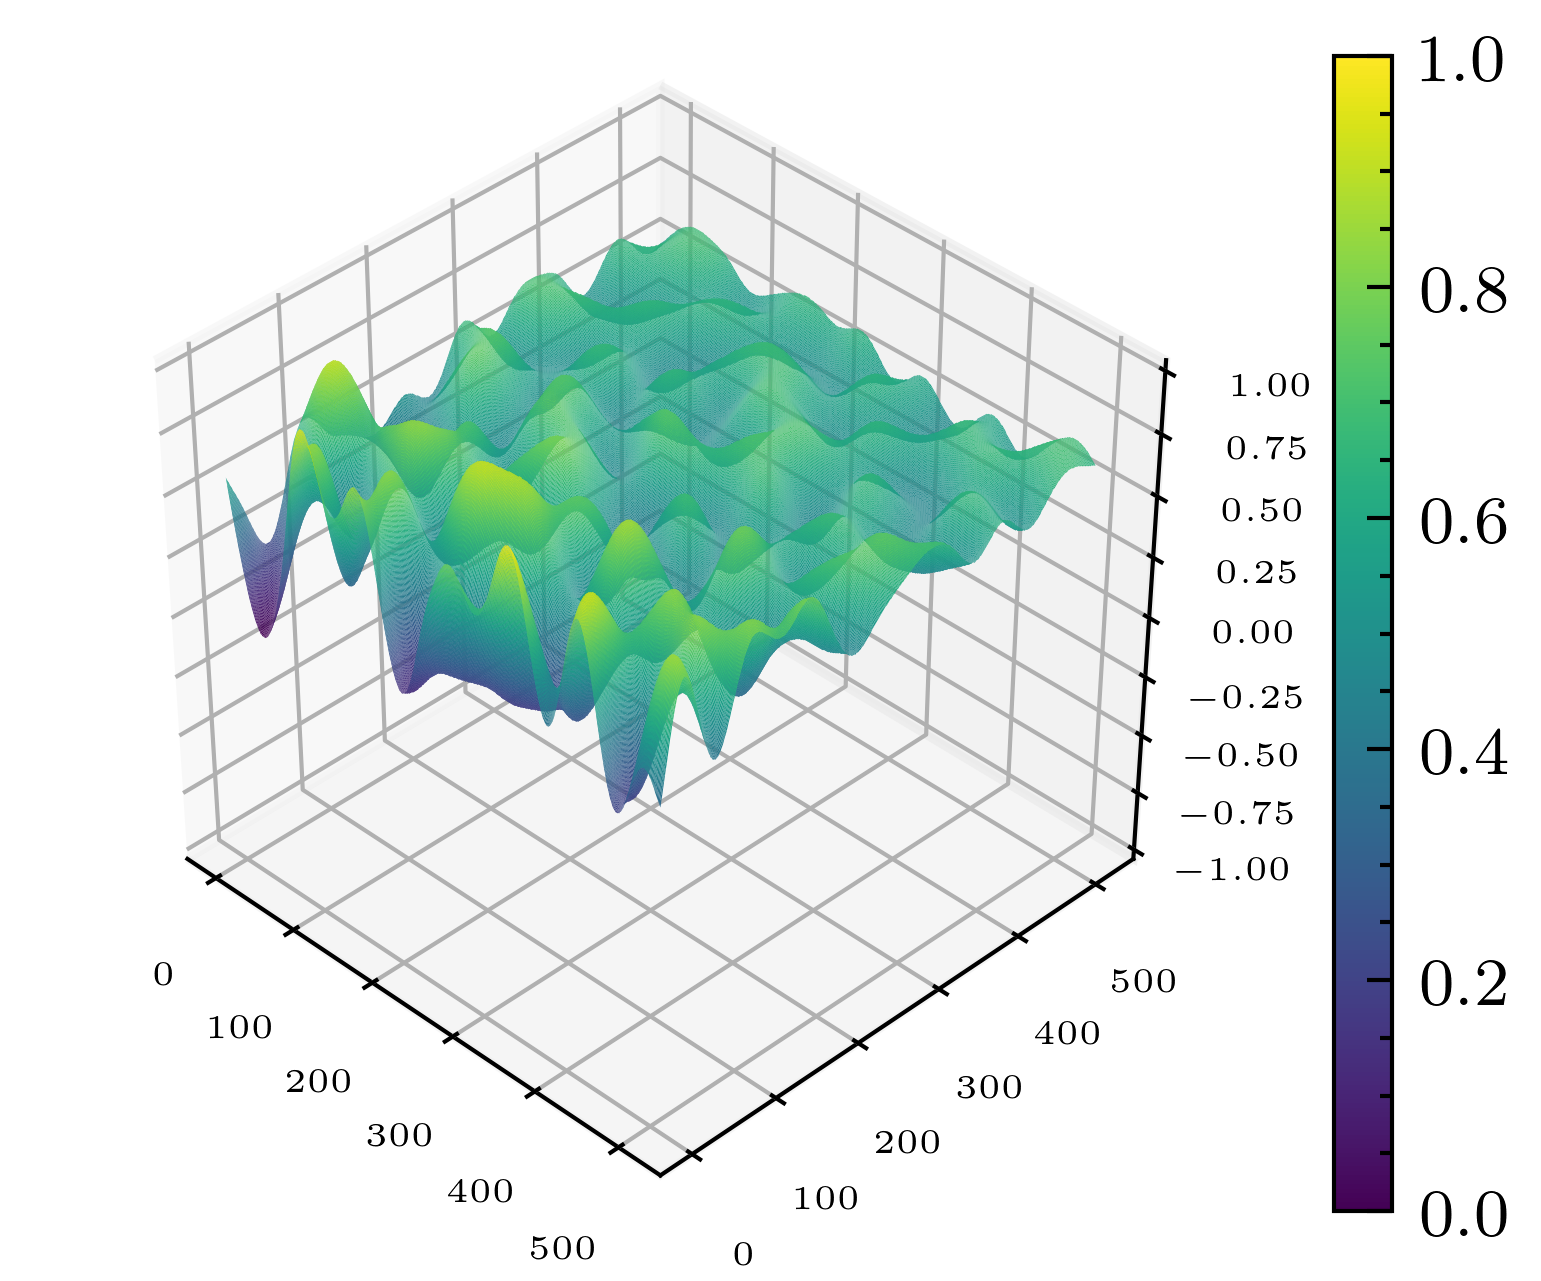
\includegraphics[width=\textwidth]{../img/hm3d/bumps2.png}
            \caption{\emph{bumps2}}
        \end{subfigure}    
        \begin{subfigure}[b]{0.32\textwidth}
            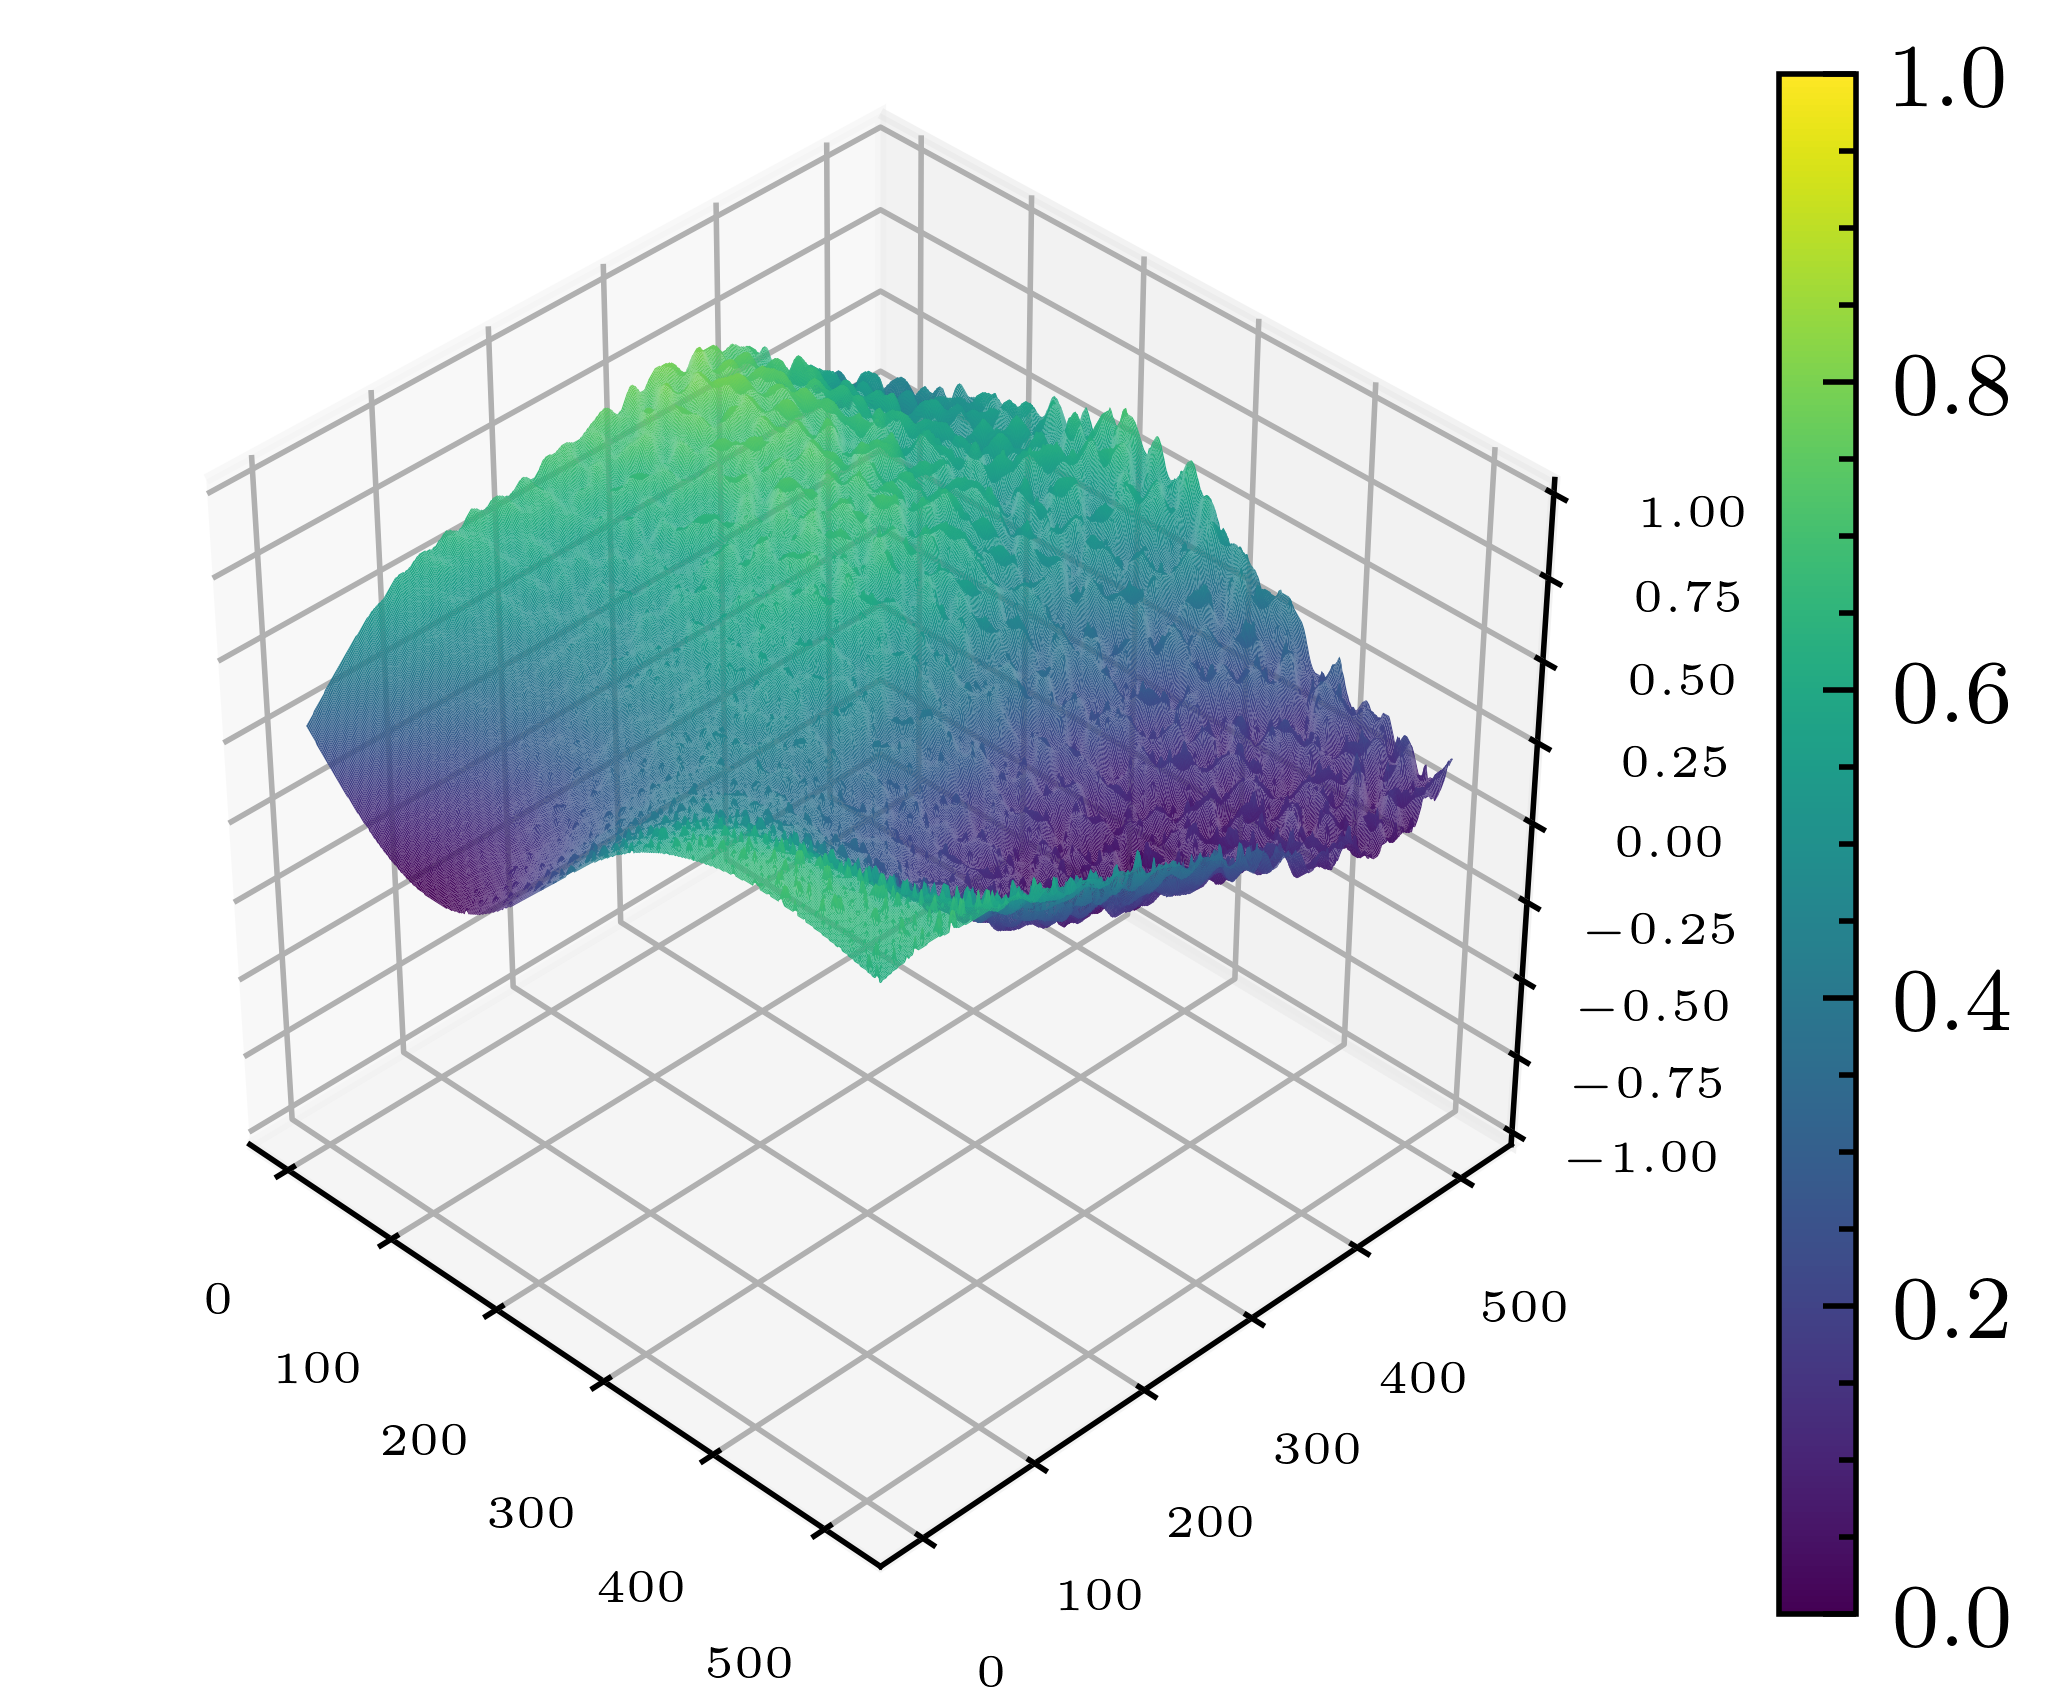
\includegraphics[width=\textwidth]{../img/hm3d/bumps3.png}
            \caption{\emph{bumps3}}
        \end{subfigure}    
    \caption{Bumps maps ($10\times10$m).}
\end{figure}
\paragraph{Bars:} In these maps there are wall with different shapes and heights. In 
\begin{figure}[H]
    \centering
        \begin{subfigure}[b]{0.32\textwidth}
            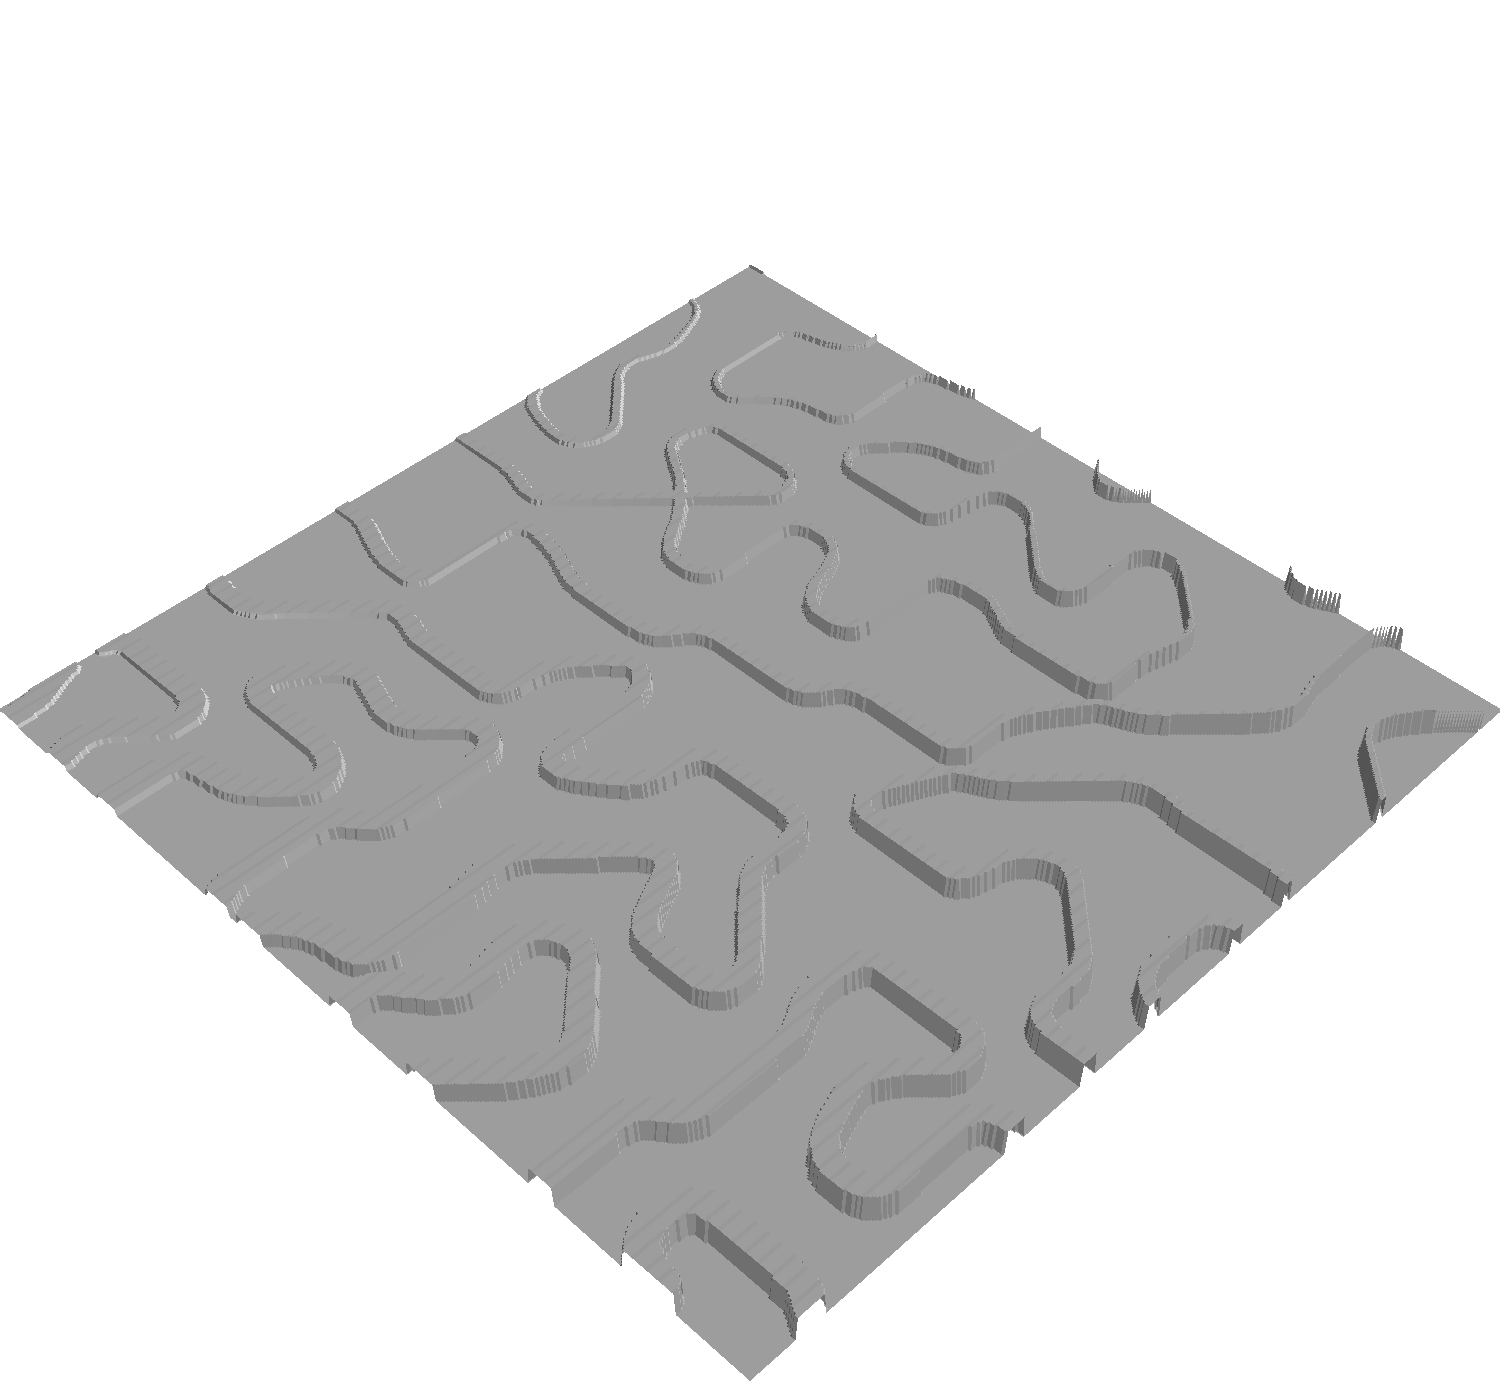
\includegraphics[width=\textwidth]{../img/hm3d/bars1.png}
            \caption{\emph{bars1}}
        \end{subfigure}
        \begin{subfigure}[b]{0.32 \linewidth}
            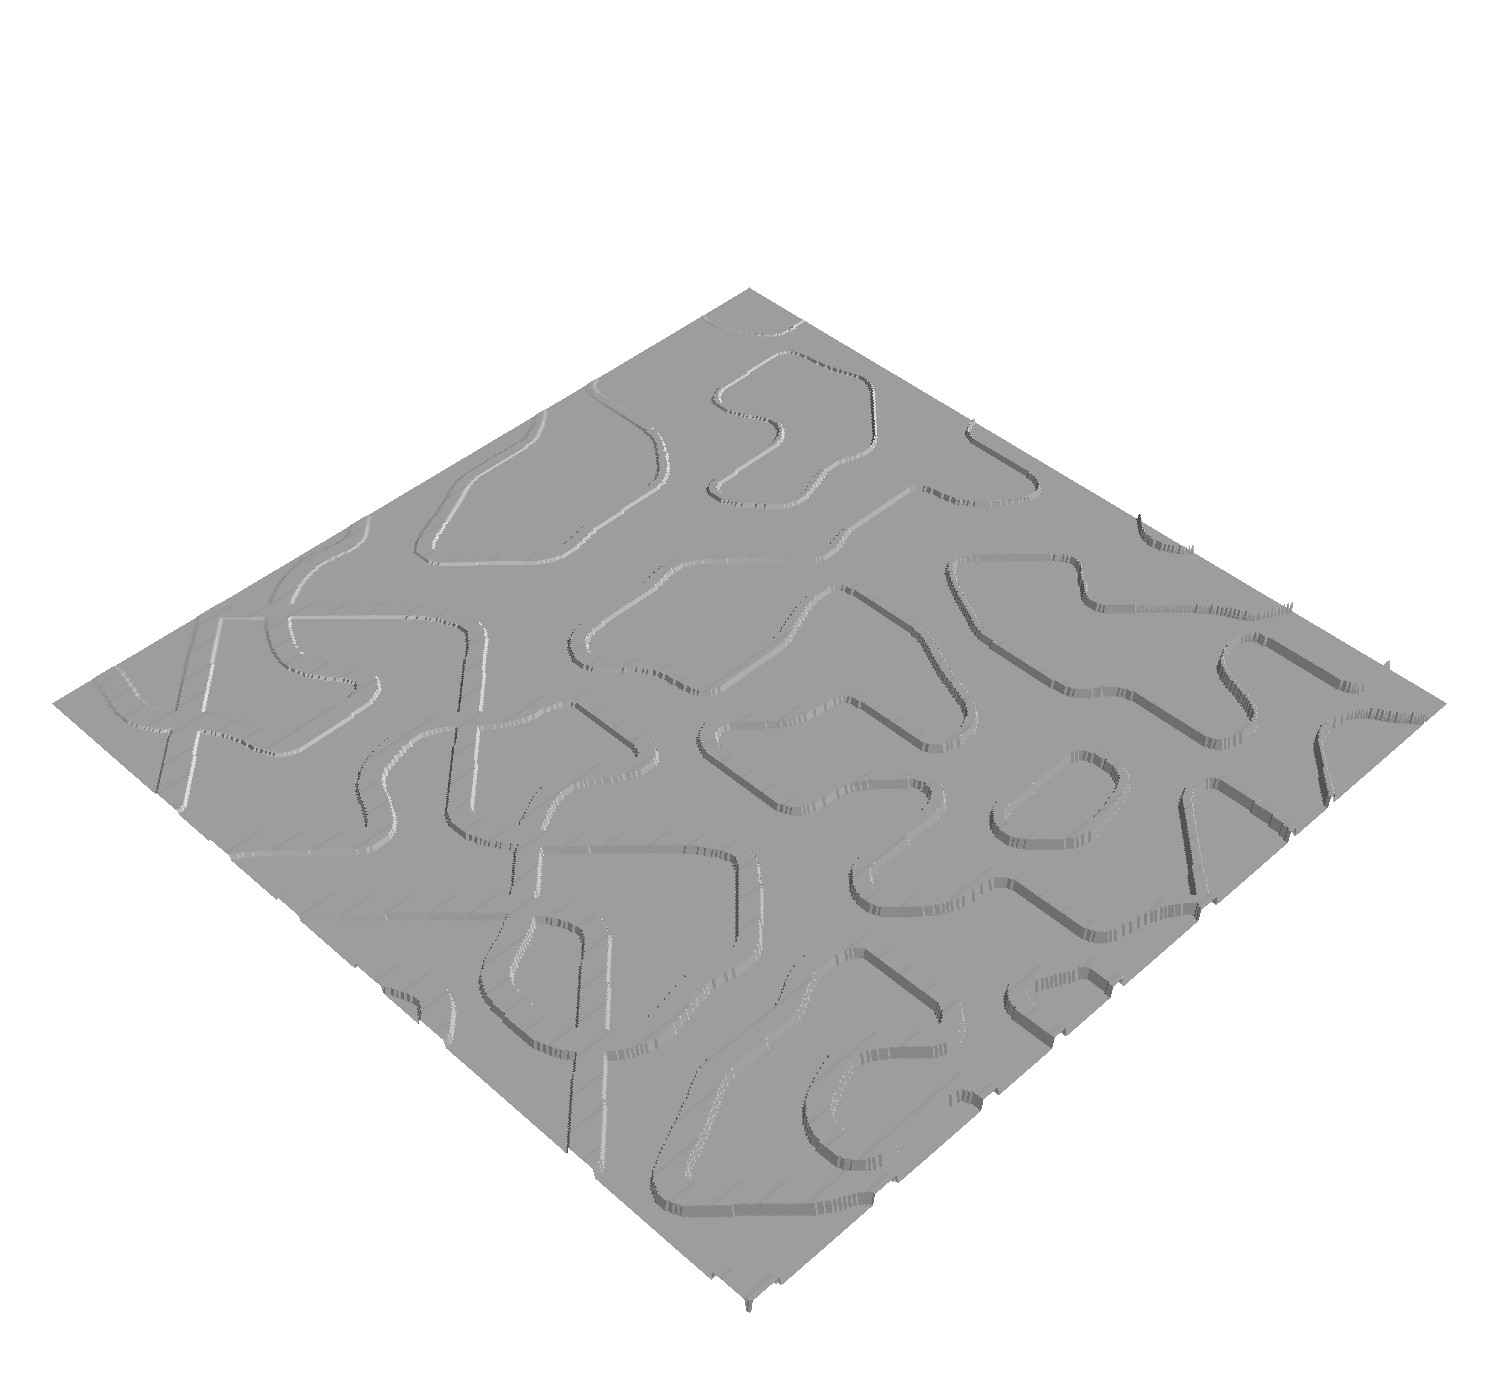
\includegraphics[width=\textwidth]{../img/hm3d/bars3.png}
            \caption{\emph{bars3}}
            \end{subfigure}     
    \caption{Bars maps ($10\times10$m).}
\end{figure}
\paragraph{Rails:} Flat grounds with slots.
\begin{figure}[H]
    \centering
        \begin{subfigure}[b]{0.32\textwidth}
            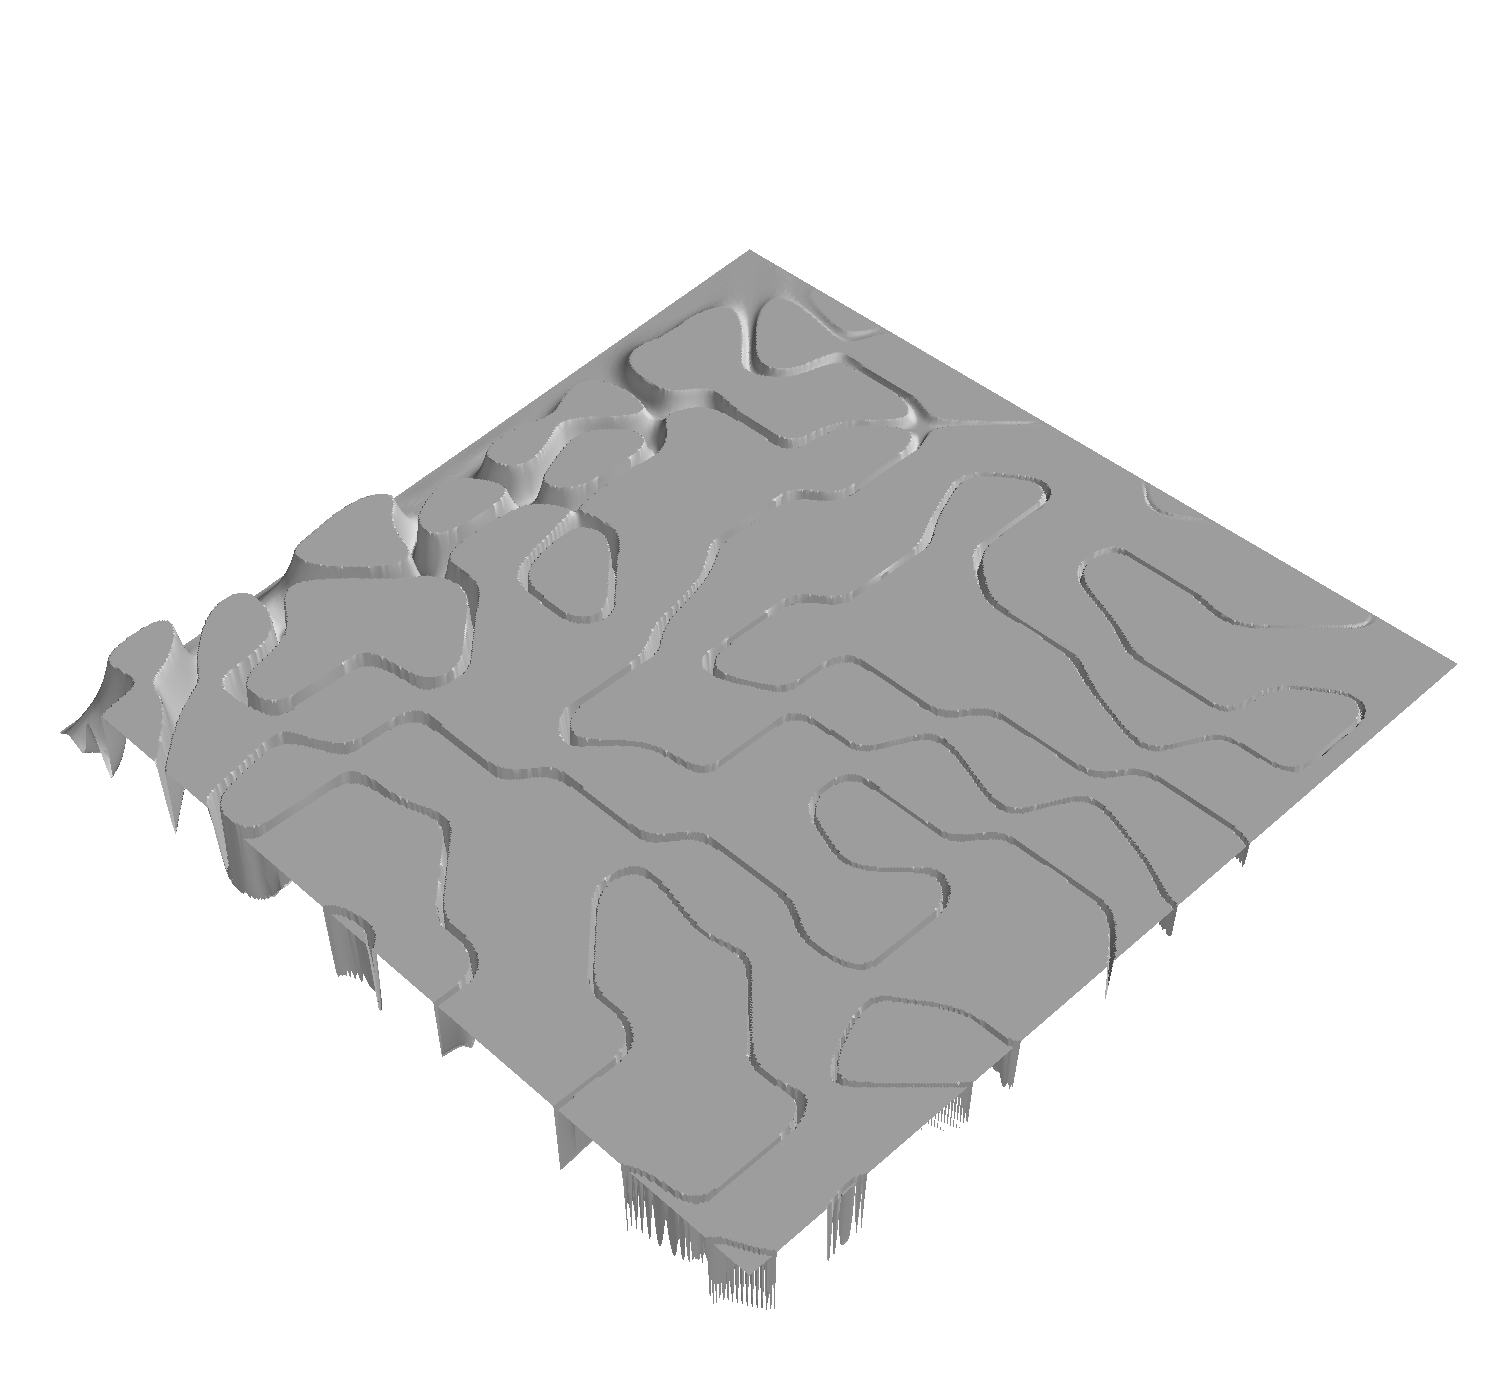
\includegraphics[width=\textwidth]{../img/hm3d/rails1.png}
            \caption{\emph{rails1}}
        \end{subfigure}
        \begin{subfigure}[b]{0.32\linewidth}
            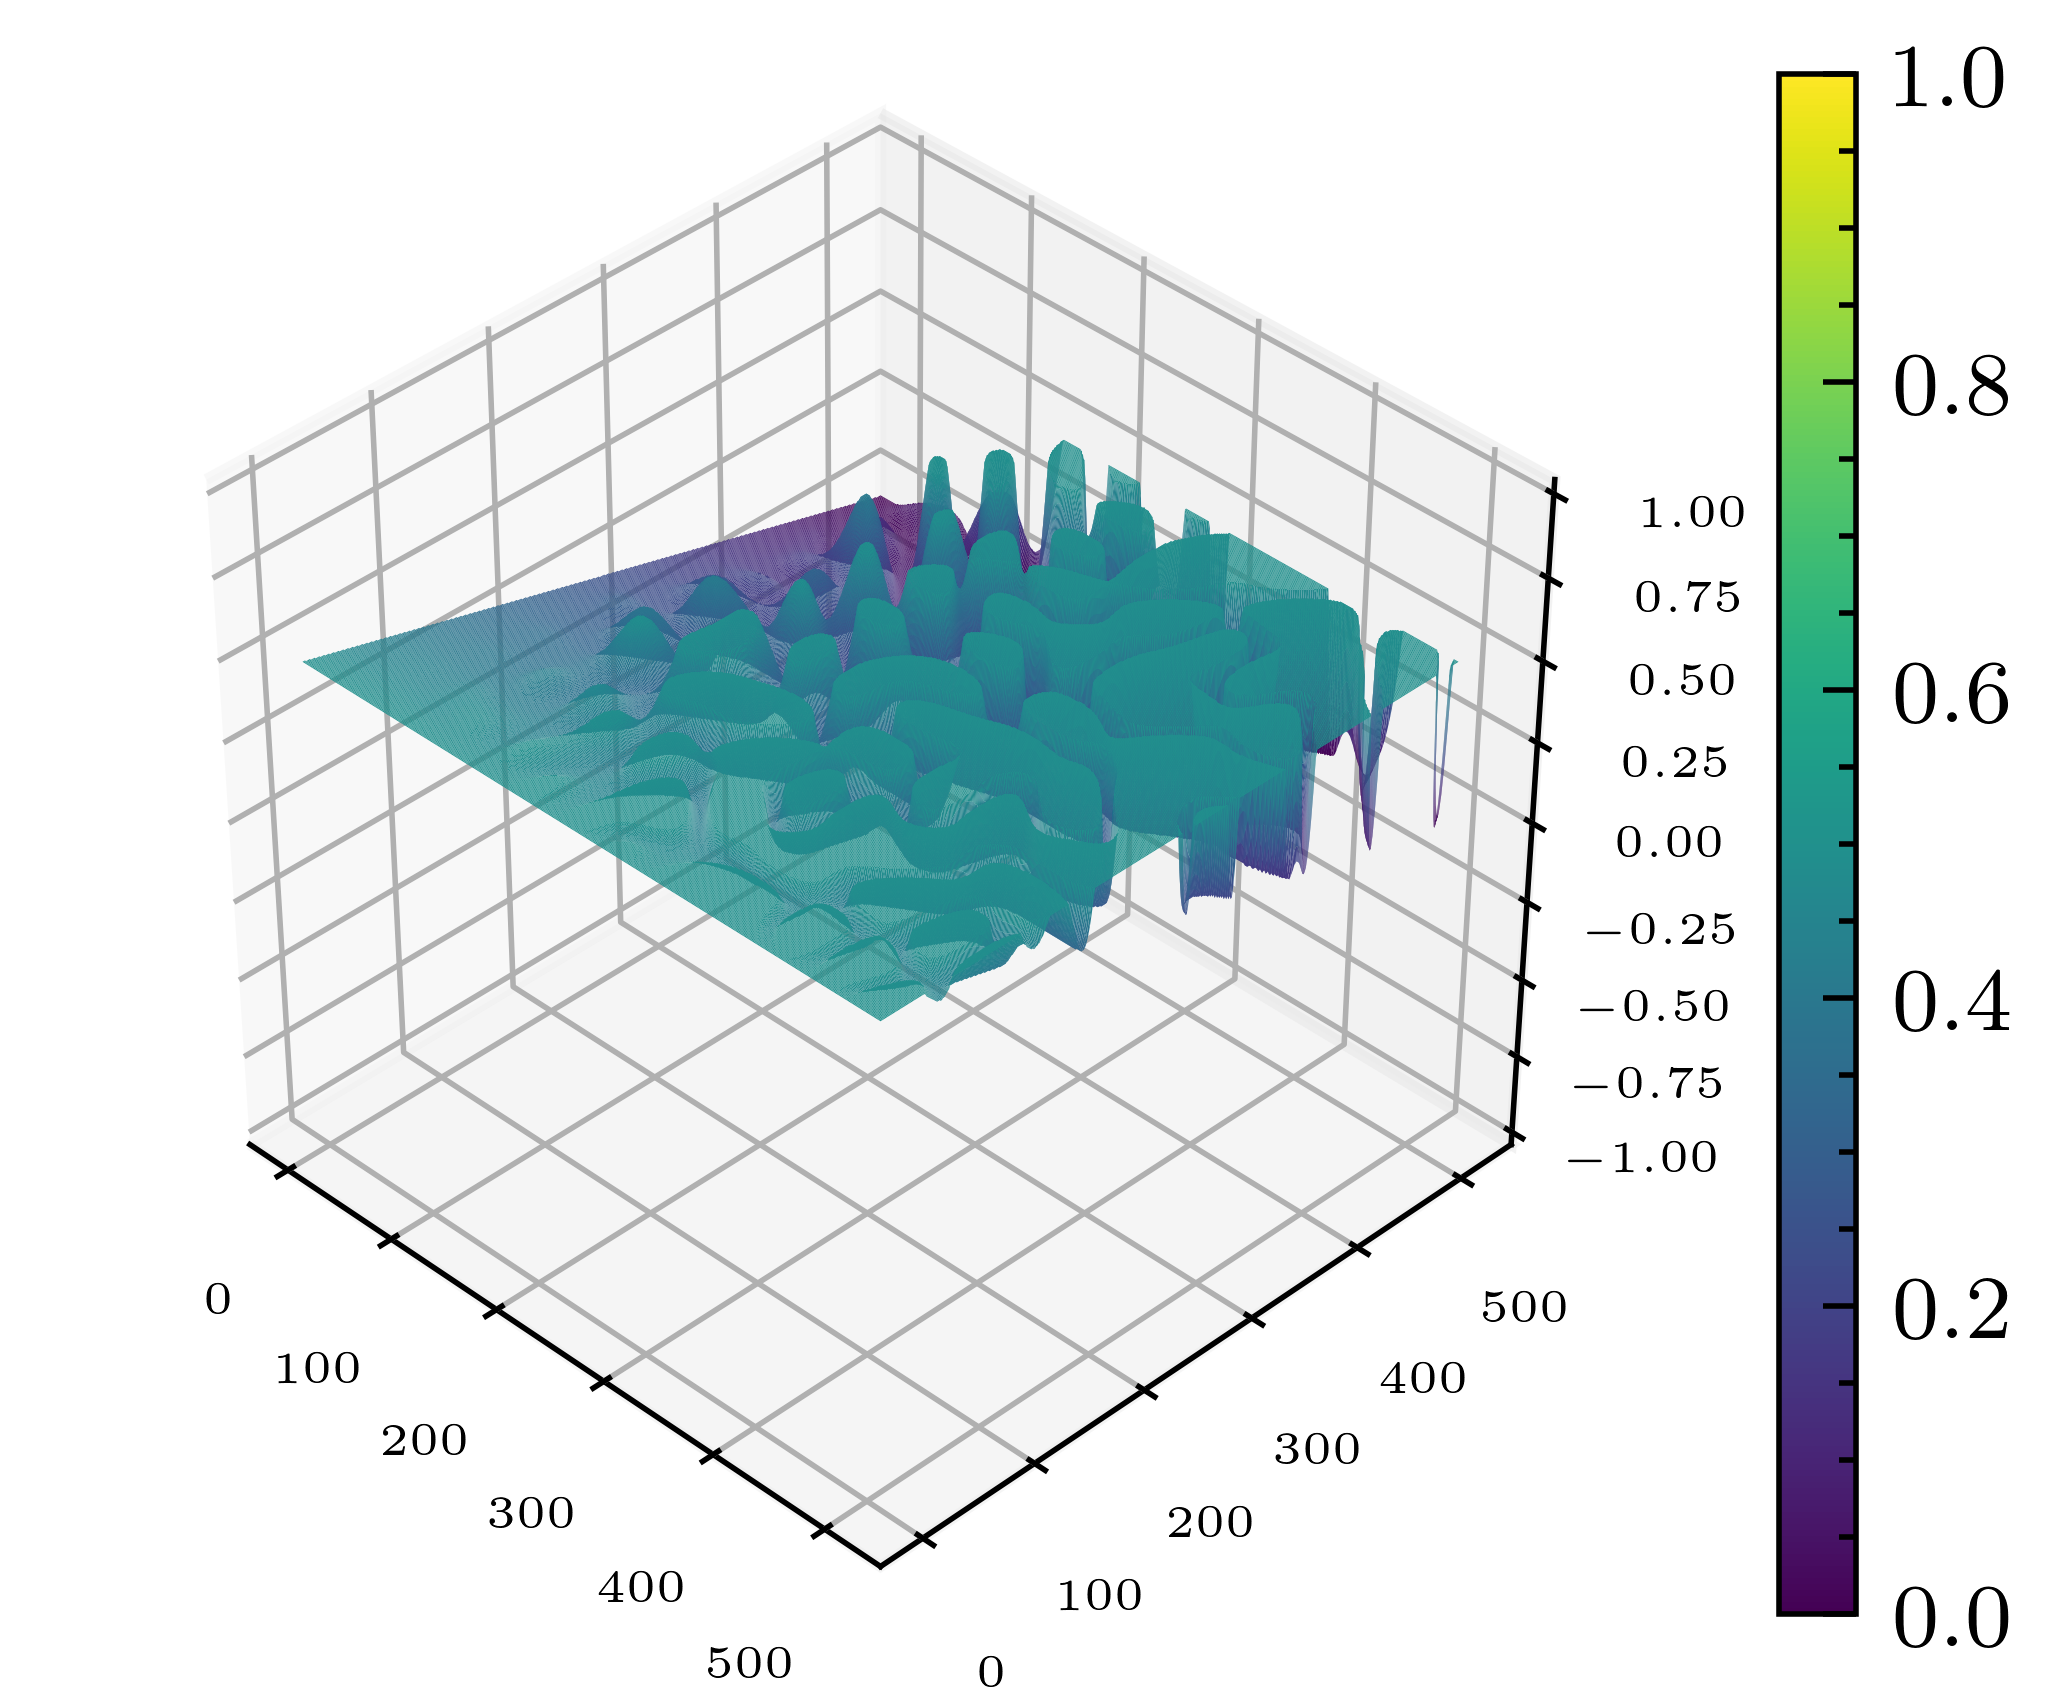
\includegraphics[width=\textwidth]{../img/hm3d/rails2.png}
            \caption{\emph{rails2}}
            \end{subfigure}    
          \begin{subfigure}[b]{0.32\textwidth}
            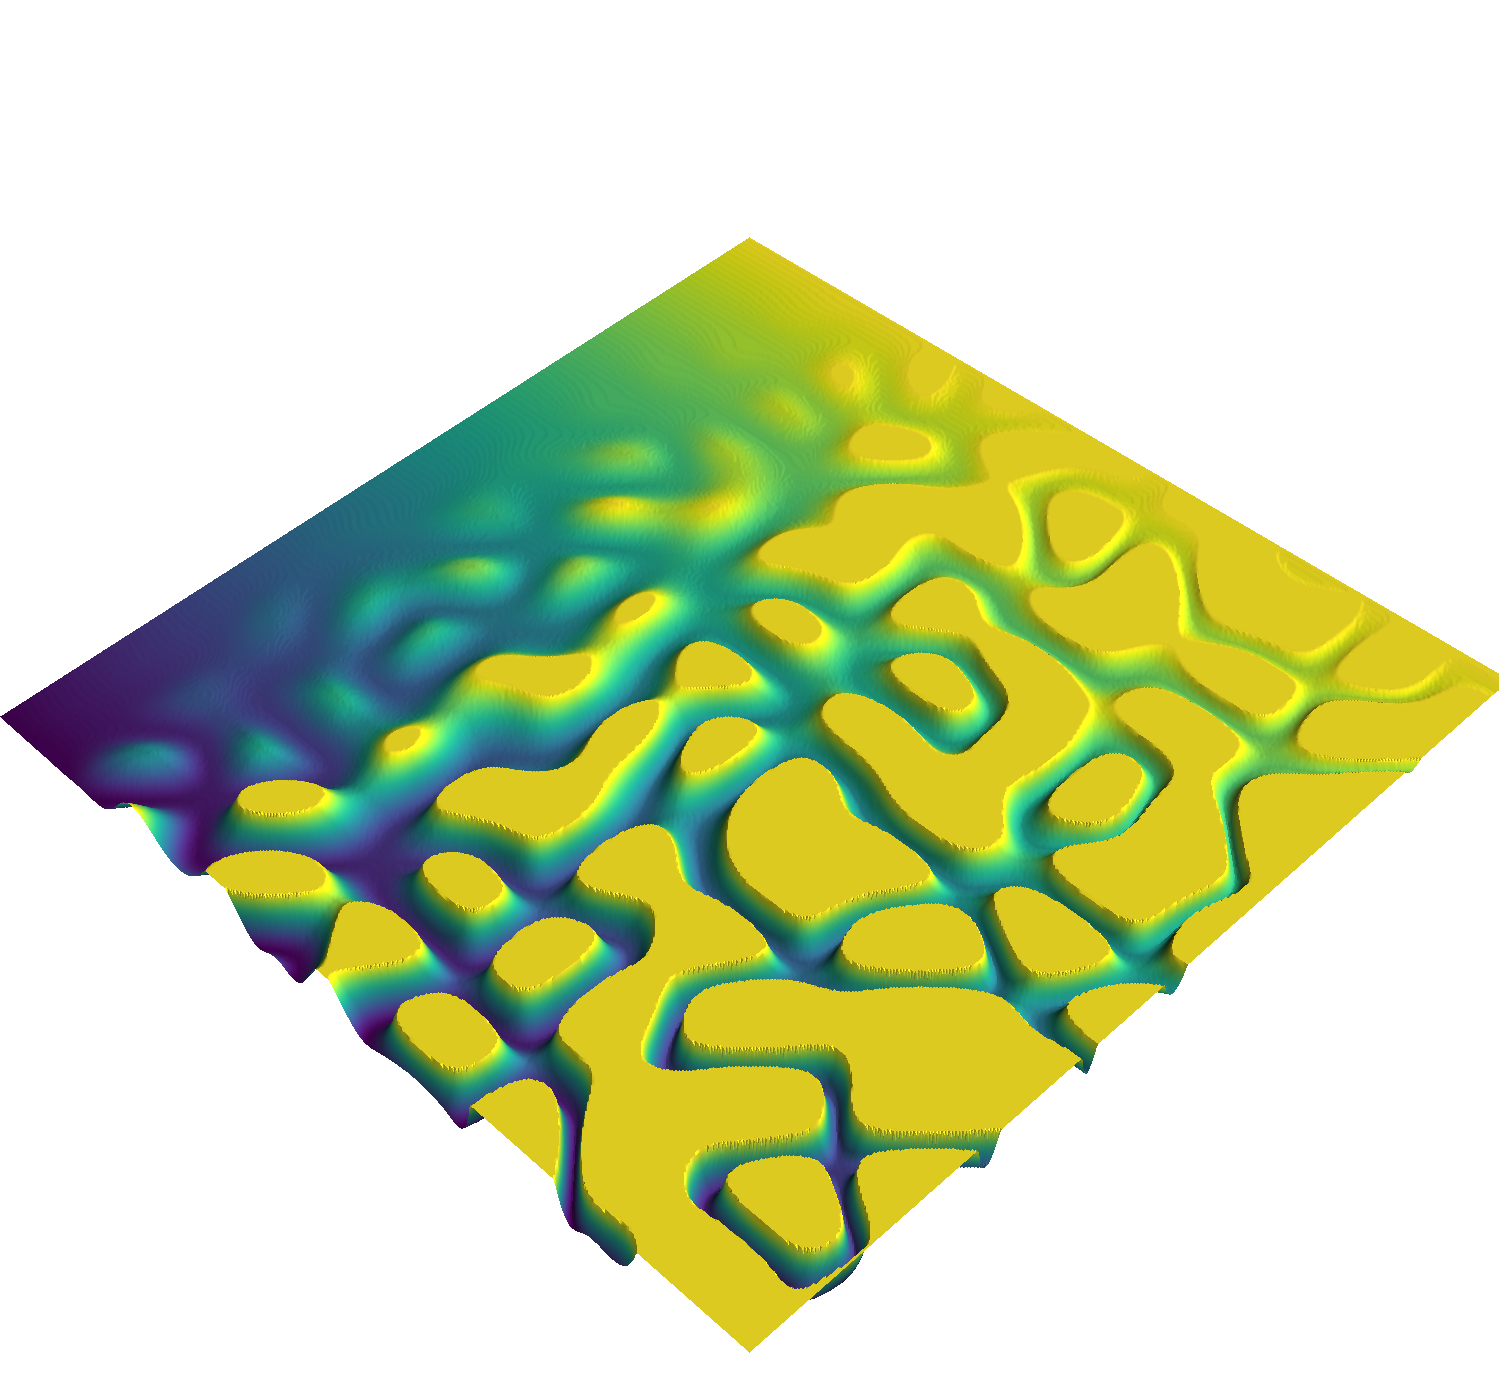
\includegraphics[width=\textwidth]{../img/hm3d/rails3.png}
            \caption{\emph{rails3}}
        \end{subfigure}    
    \caption{Rails maps ($10\times10$m).}
\end{figure}
\paragraph{Steps:} These are maps have huge wall and holes
\begin{figure}[H]
    \centering
        \begin{subfigure}[b]{0.32\textwidth}
            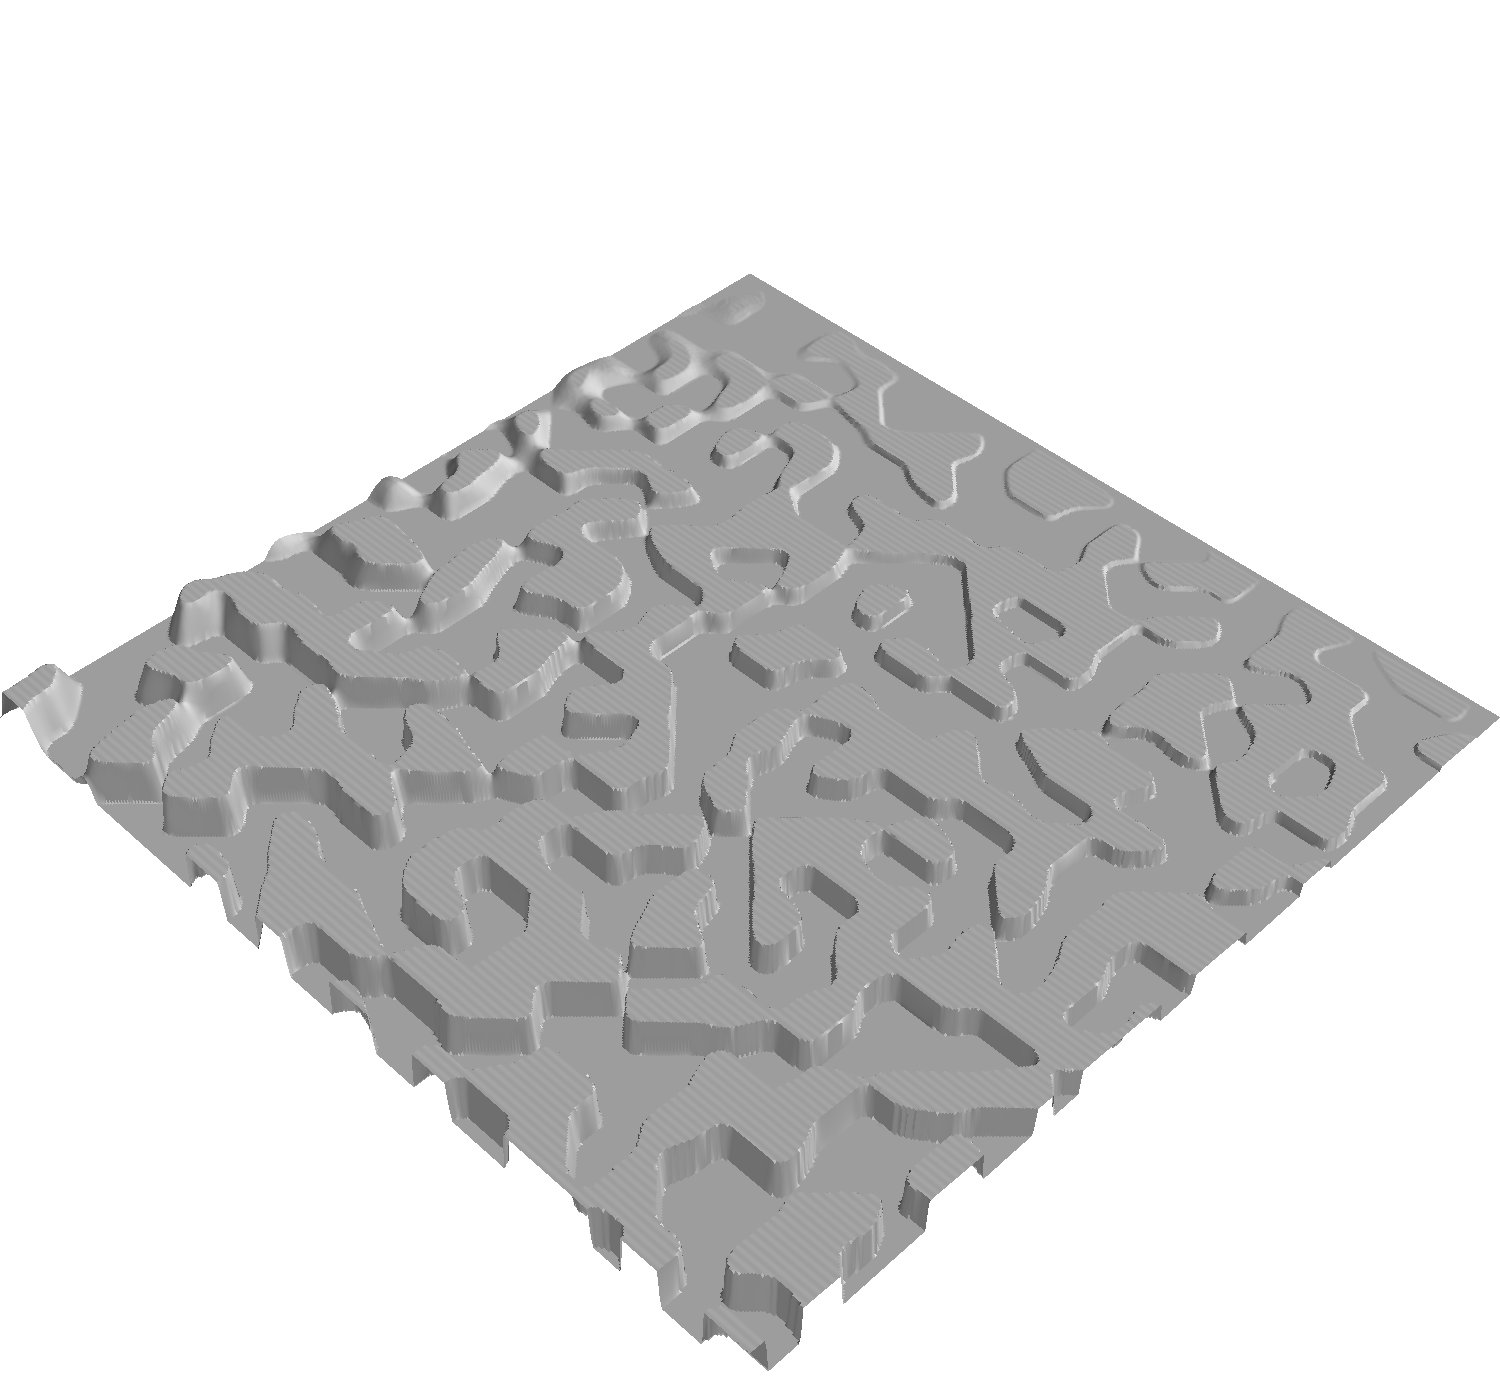
\includegraphics[width=\textwidth]{../img/hm3d/steps1.png}
            \caption{\emph{steps1}}
        \end{subfigure}
        \begin{subfigure}[b]{0.32\linewidth}
            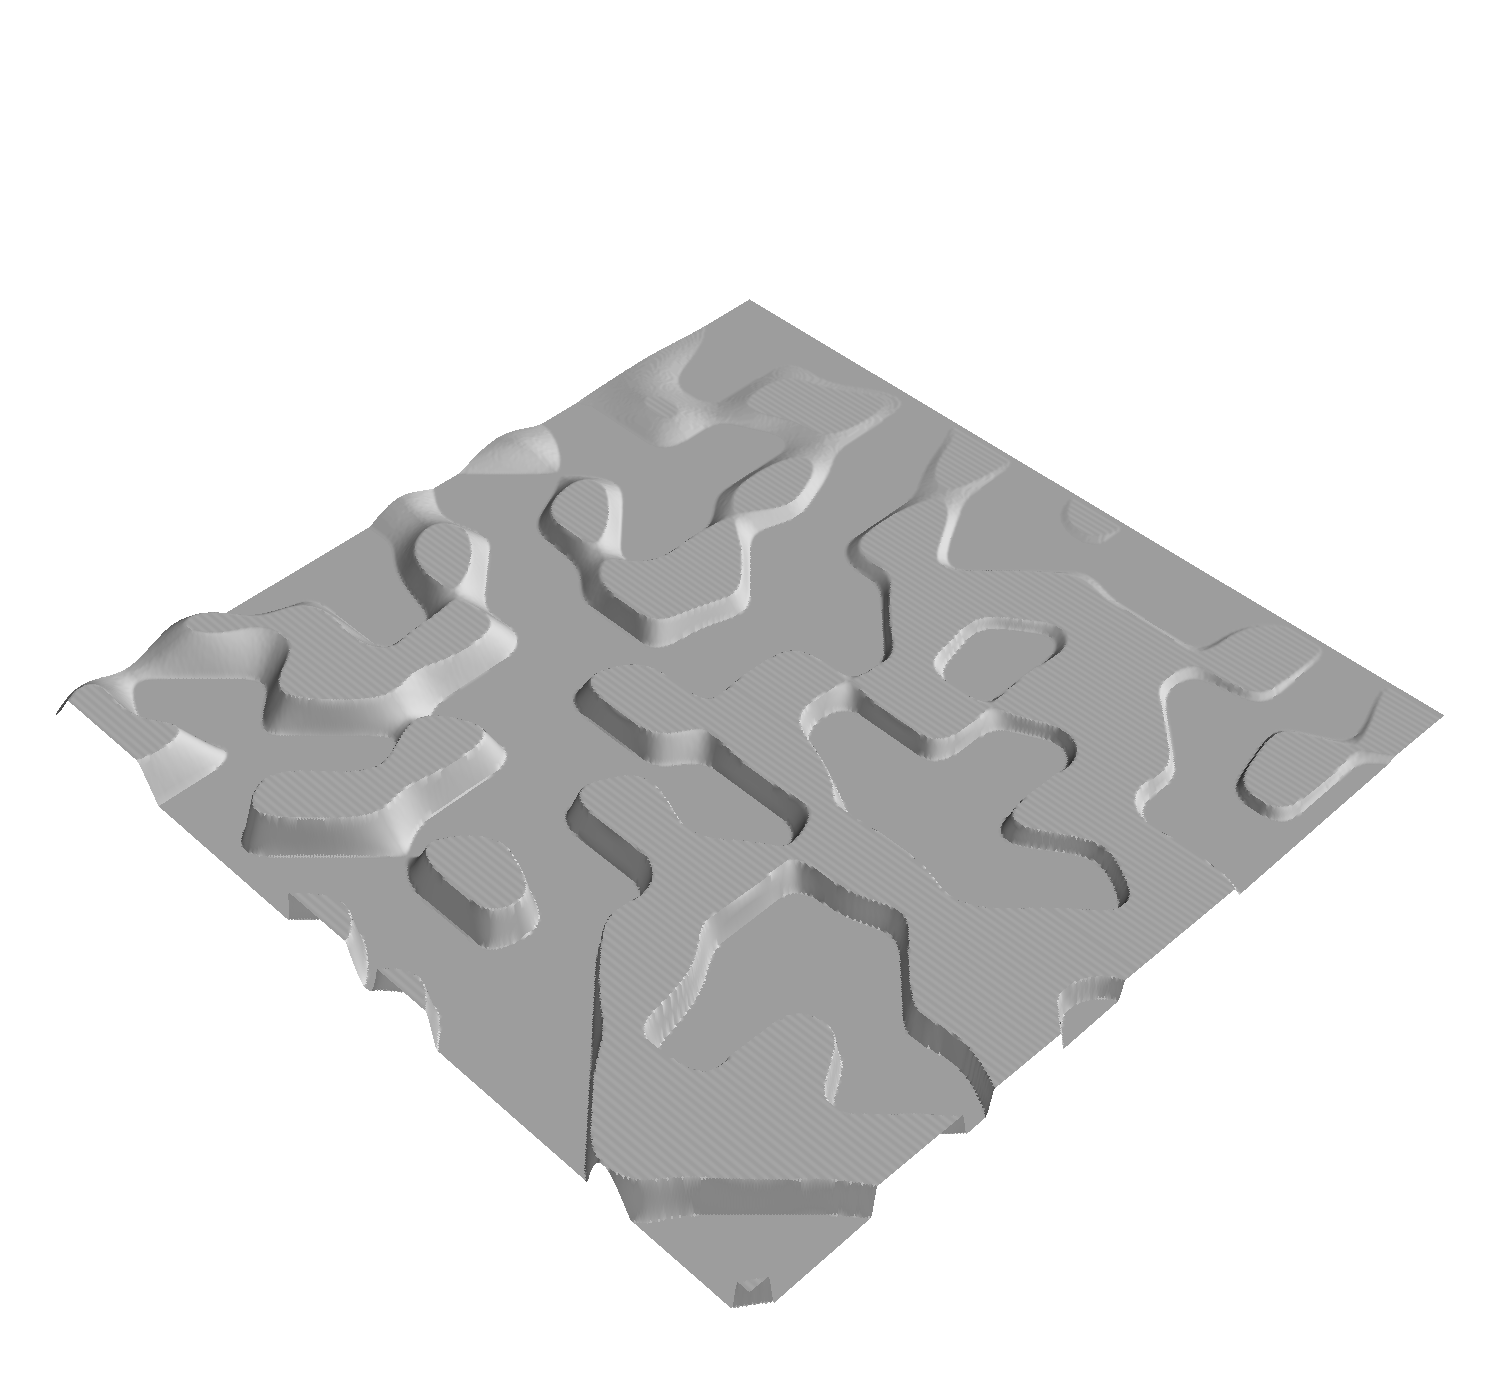
\includegraphics[width=\textwidth]{../img/hm3d/steps2.png}
            \caption{\emph{steps2}}
            \end{subfigure}    
          \begin{subfigure}[b]{0.32\textwidth}
            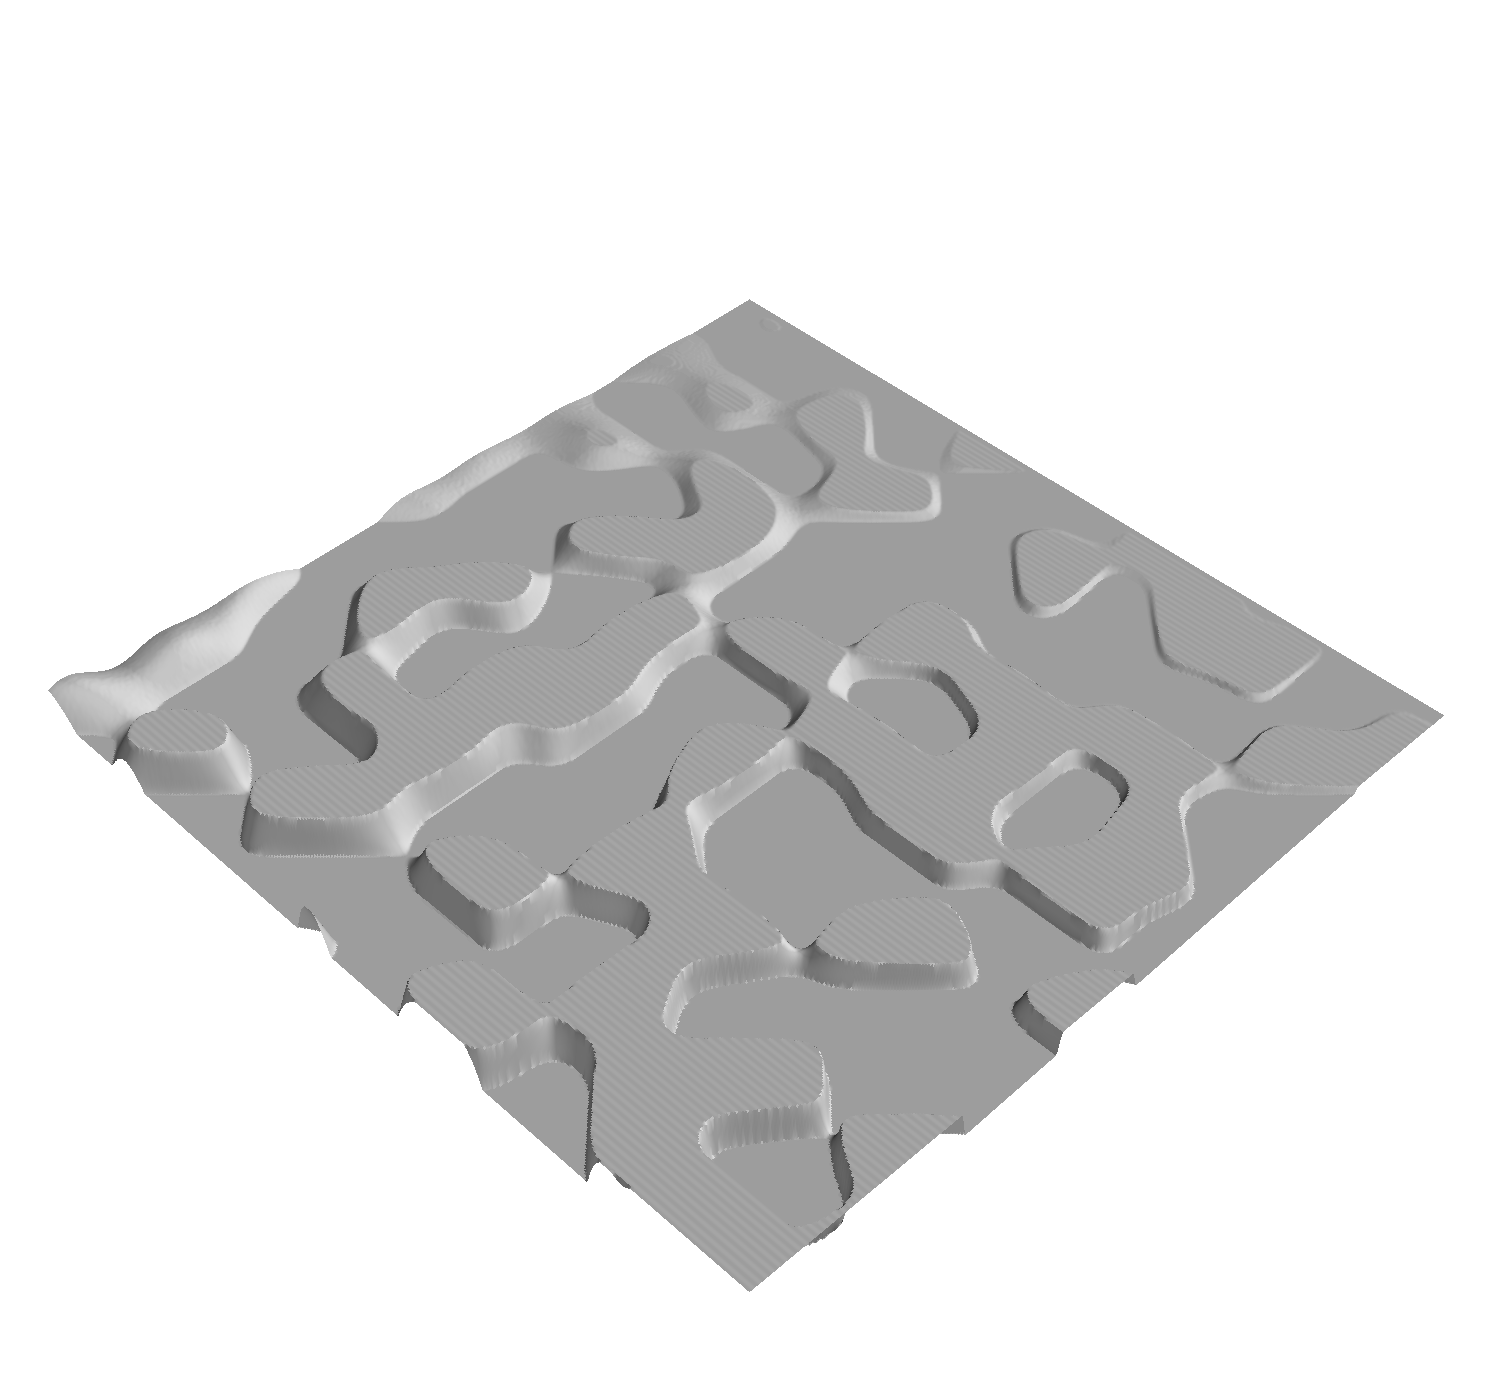
\includegraphics[width=\textwidth]{../img/hm3d/steps3.png}
            \caption{\emph{steps3}}
        \end{subfigure}    
    \caption{Steps maps ($10\times10$m).}
\end{figure}

\paragraph{Slopes/Ramps:} Maps composed by uneven terrain scaled by different height factors from $3$ to $5$ used to include samples where \emph{Krock} has to climb. Those maps were scaled up with different height factors.
\begin{figure}[H]
    \centering
        \begin{subfigure}[b]{0.32\textwidth}
            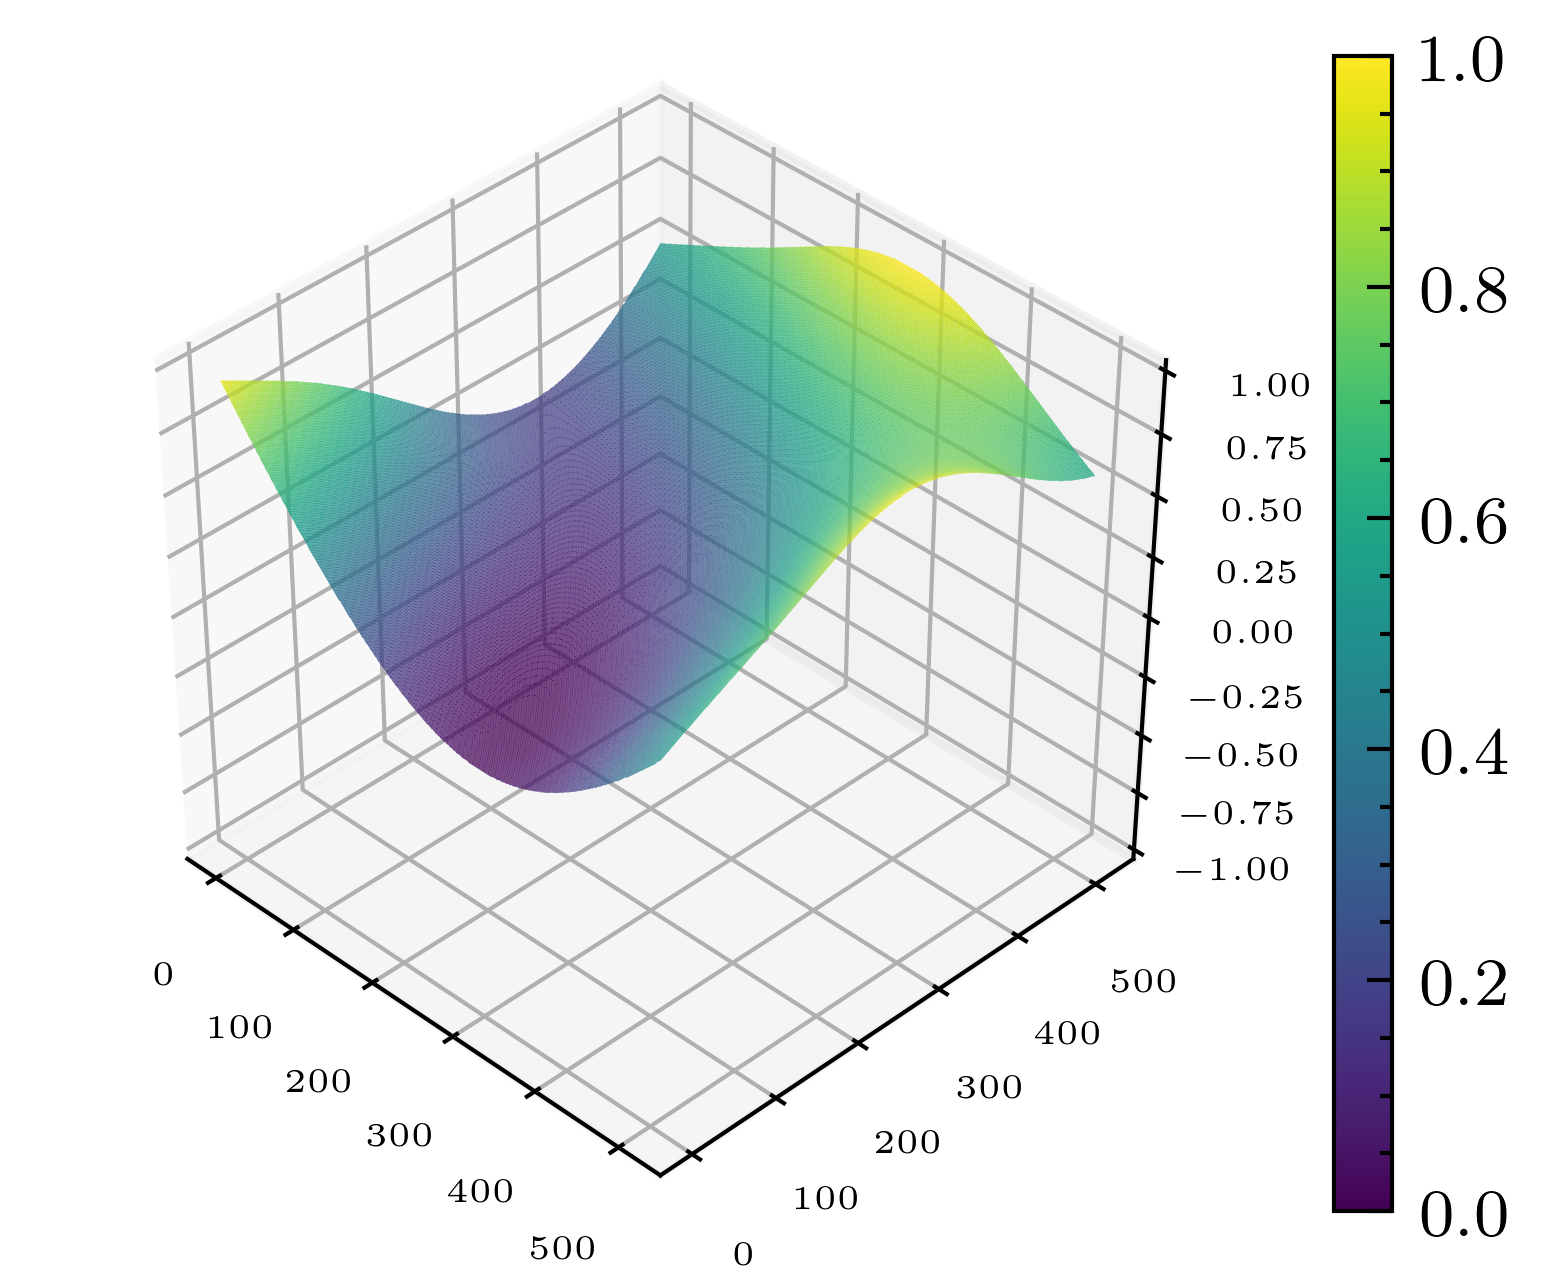
\includegraphics[width=\textwidth]{../img/hm3d/ramp0.png}
            \caption{\emph{ramp0}}
        \end{subfigure}
        \begin{subfigure}[b]{0.32\linewidth}
            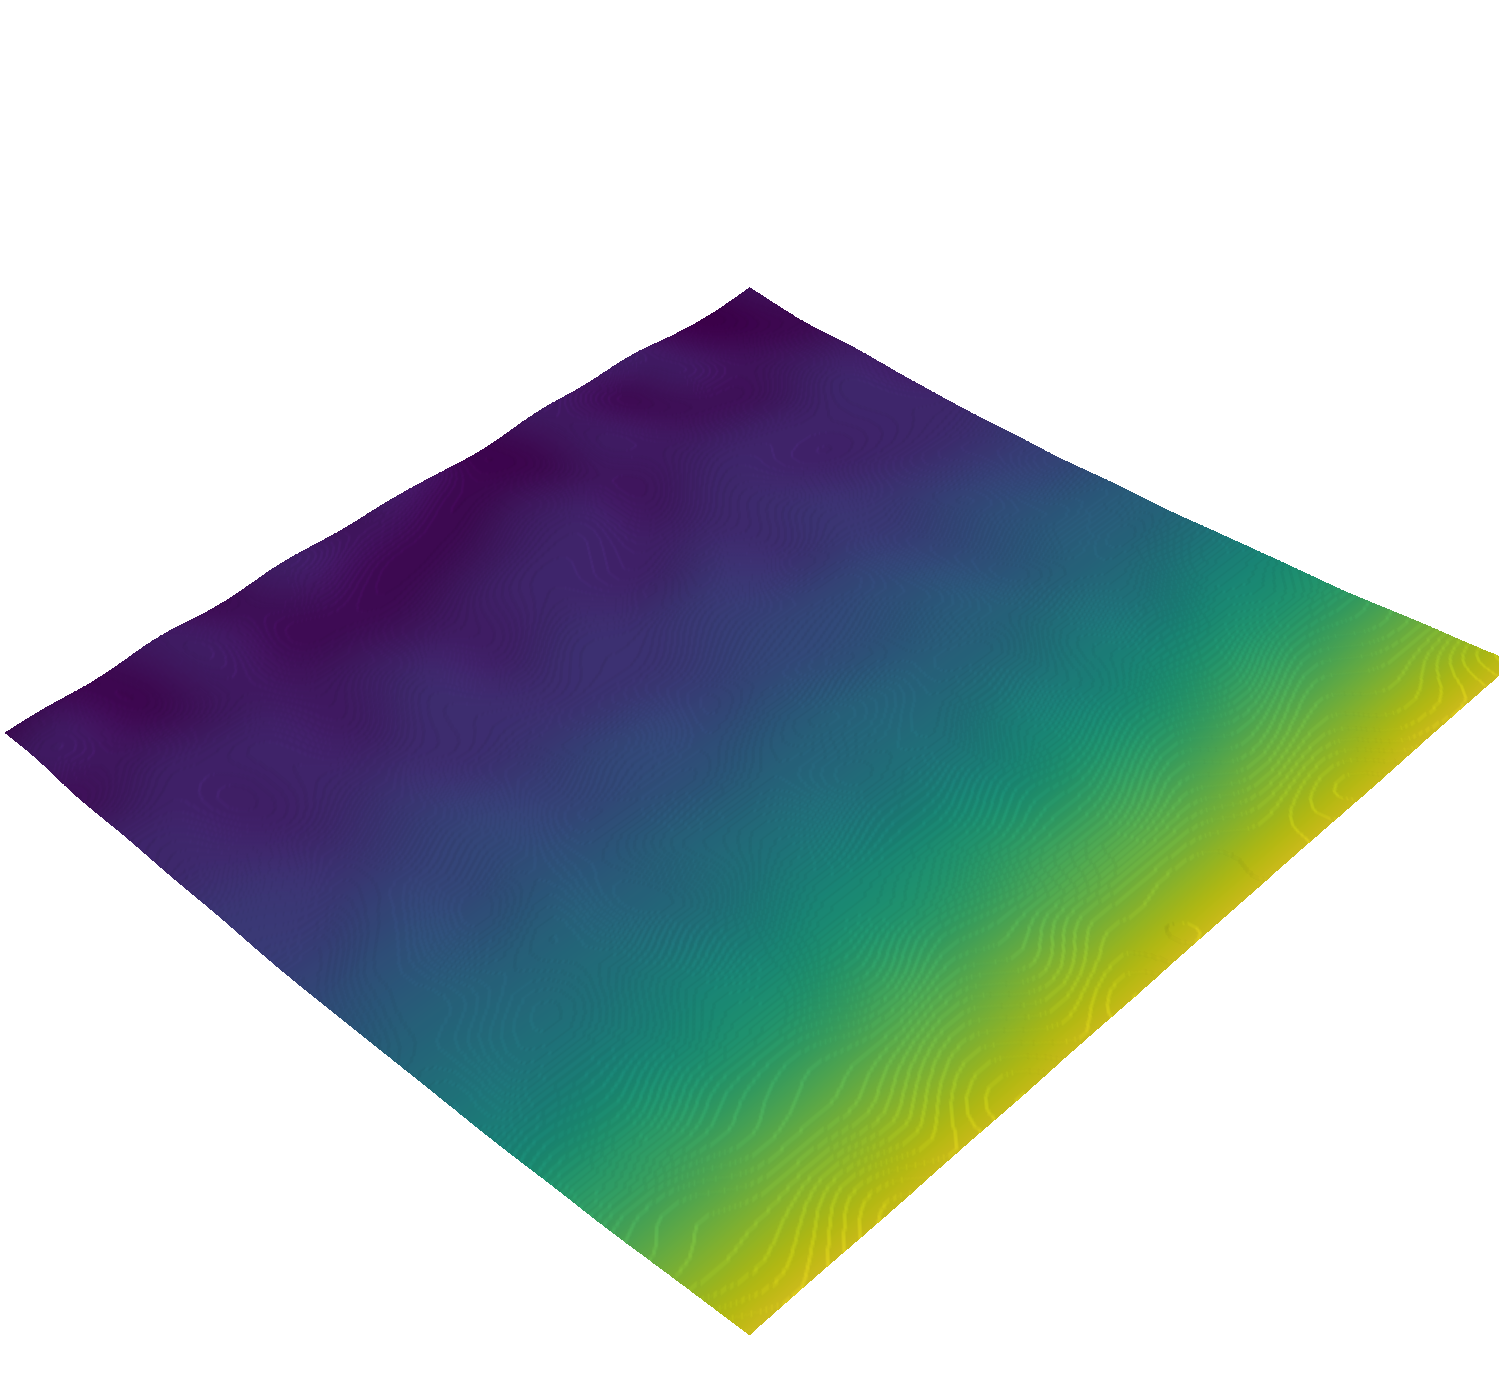
\includegraphics[width=\textwidth]{../img/hm3d/ramp1.png}
            \caption{\emph{ramp1}}
            \end{subfigure}    
          \begin{subfigure}[b]{0.32\textwidth}
            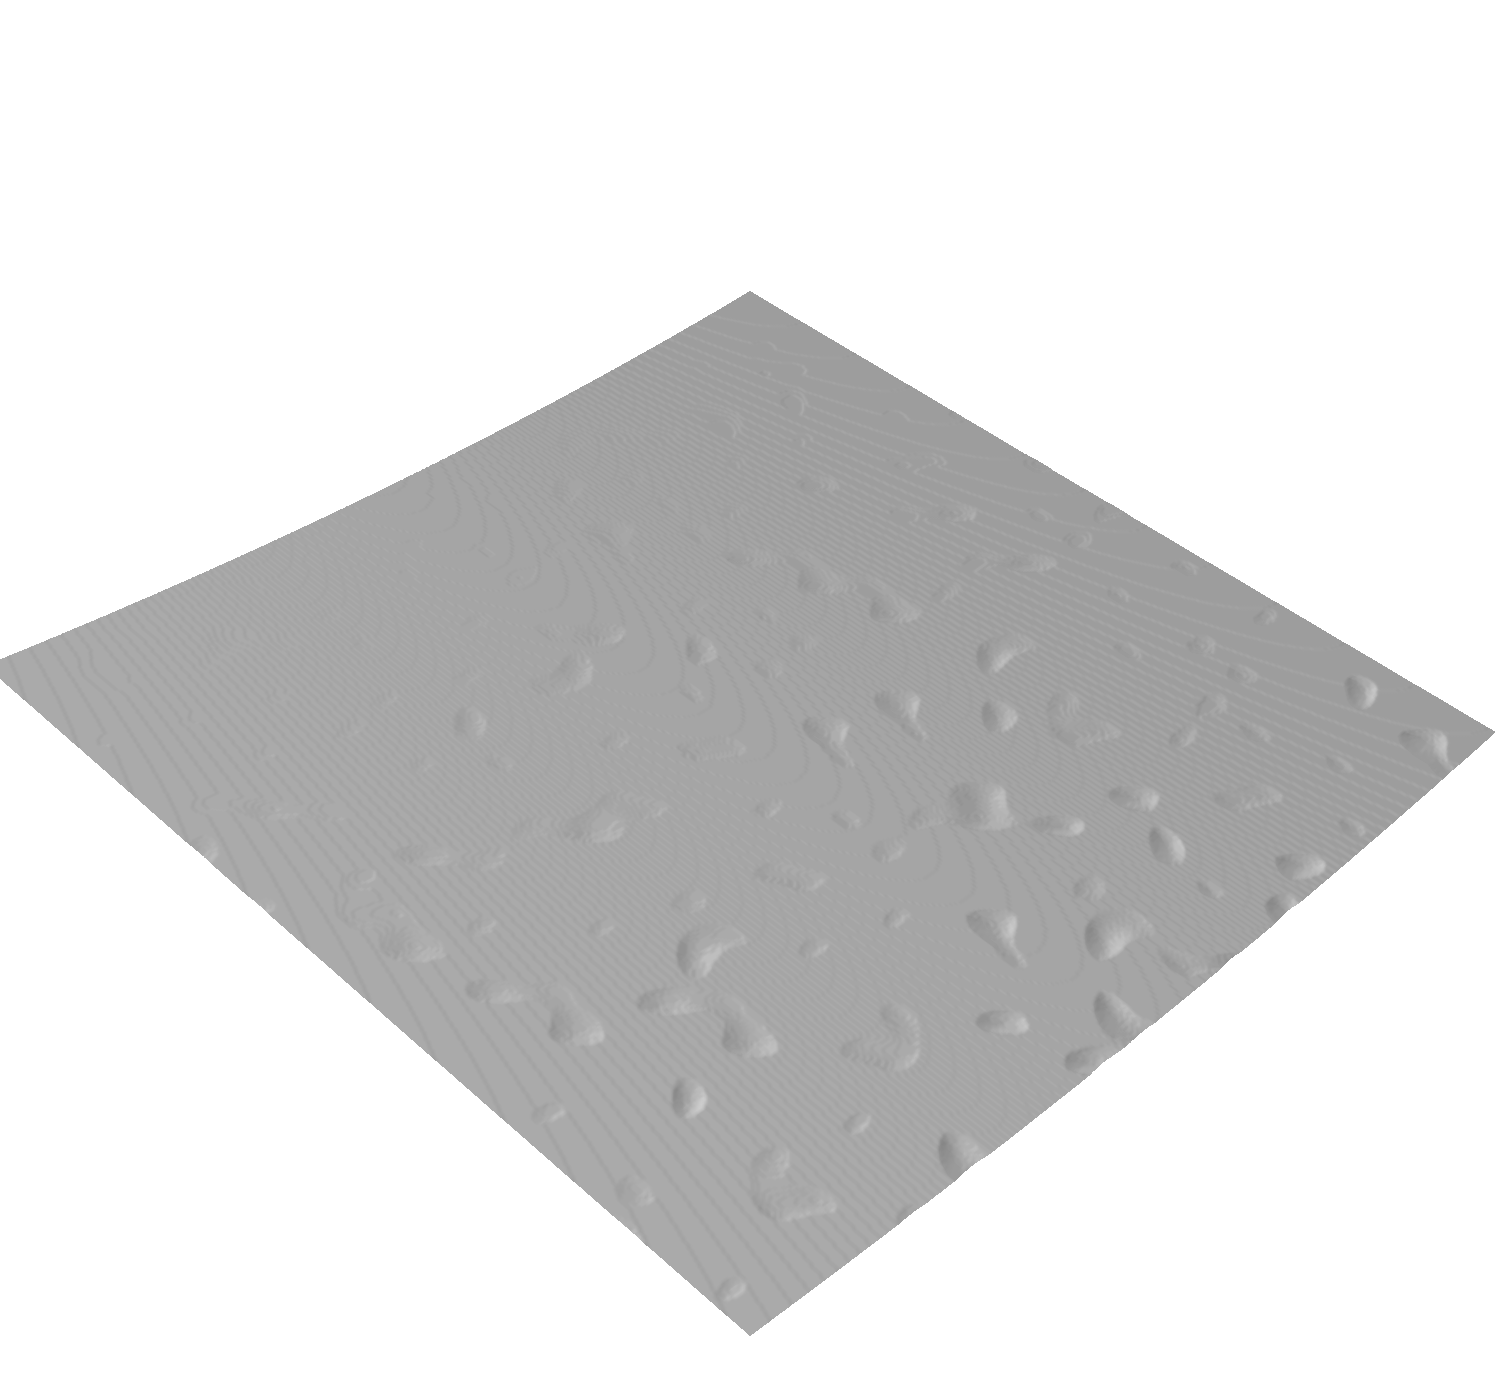
\includegraphics[width=\textwidth]{../img/hm3d/slope_rocks1.png}
            \caption{\emph{slope\_rocks1}}
        \end{subfigure}    
    \caption{Slopes maps ($10\times10$m).}
\end{figure}
\paragraph{Holes} We also included a map with holes
\begin{figure}[H]
    \centering
        \begin{subfigure}[b]{0.32\textwidth}
            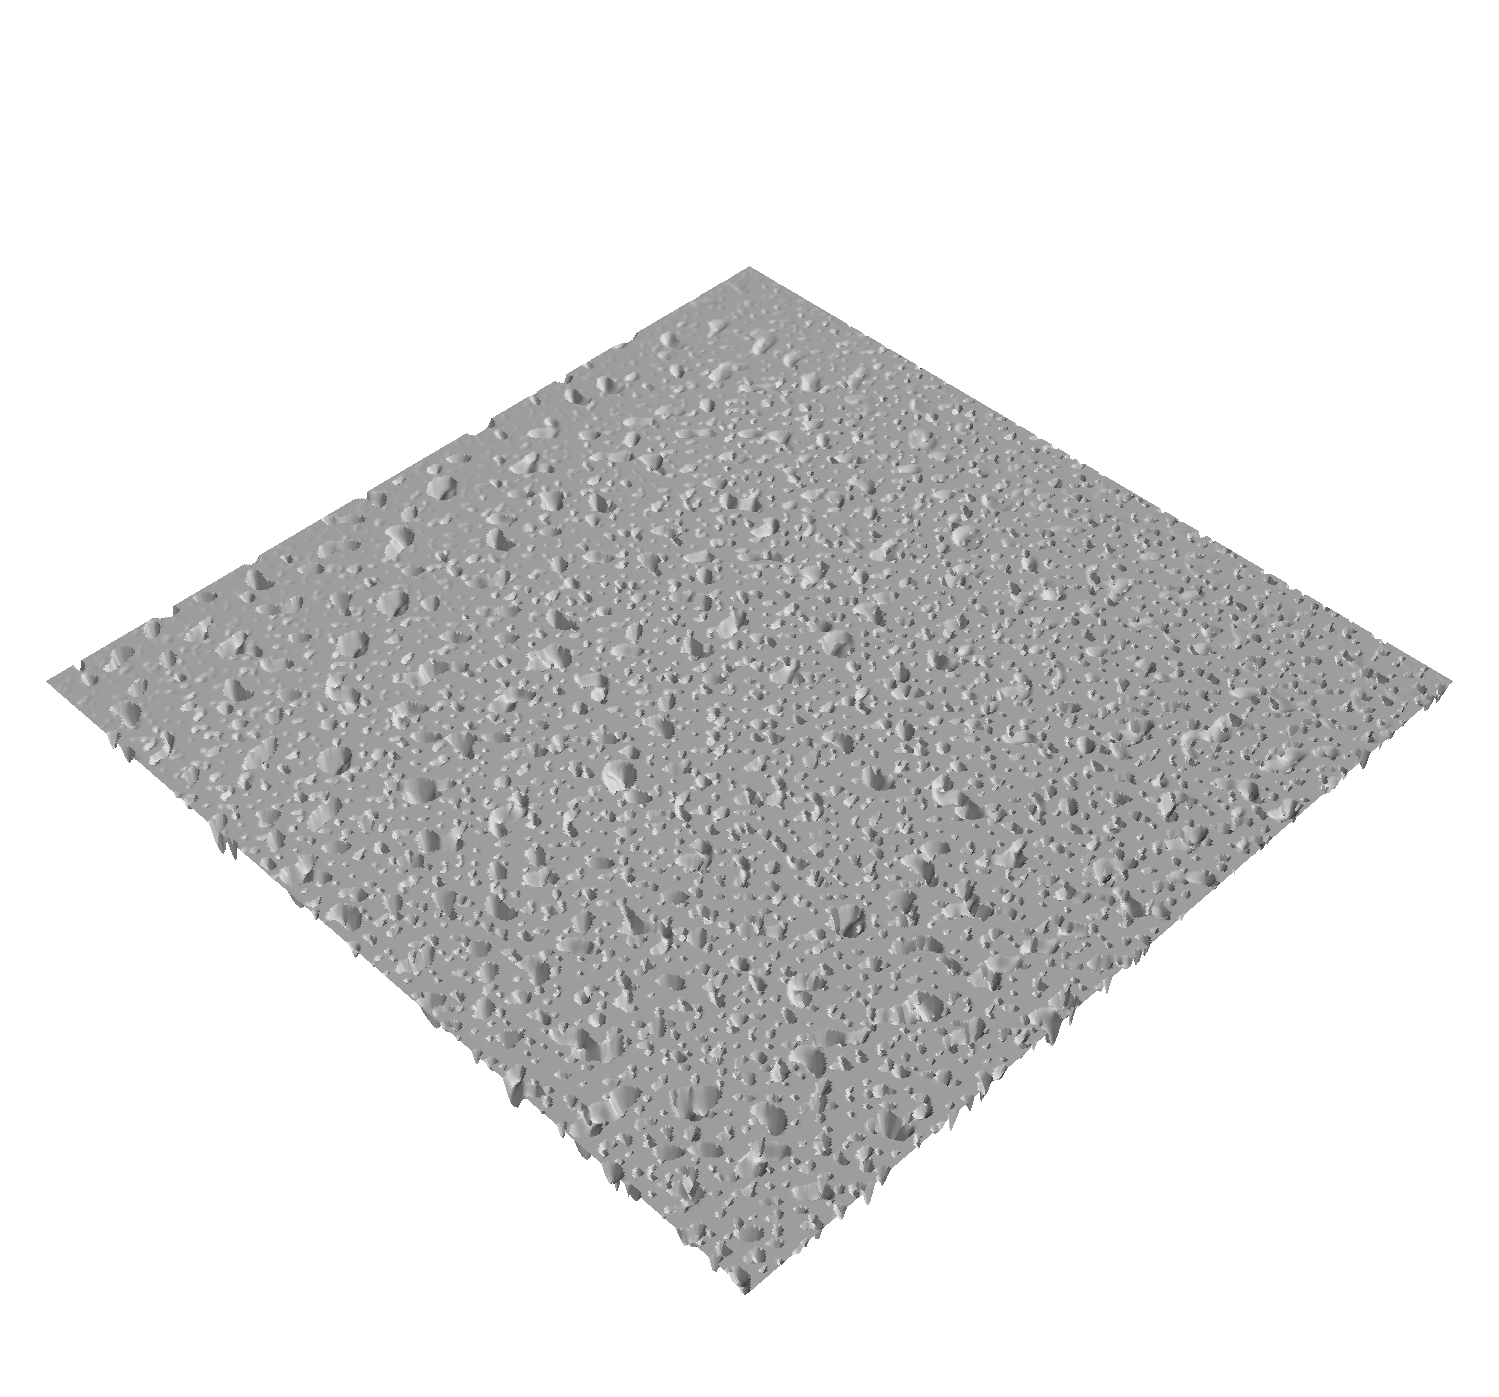
\includegraphics[width=\textwidth]{../img/hm3d/holes1.png}
            \caption{\emph{holes1}}
        \end{subfigure}
\caption{Holes map ($10\times10$m).}
\end{figure}
\subsubsection{Simulator}
We used Webots to move \emph{Krock} on the genereted terrain. The robot controlled was implemented by EPFL \todo{cite them?} and handed to IDSIA \todo{cite?}. The controller implements a ROS' node to publish \emph{Krock} status including its pose at a rate of $250hz$. We decide to reduce it $50hz$ by using ROS build it \texttt{throttle} command. 
To load the map into the simulator, we fist had to convert it to Webots's \emph{.wbt} file. Unfortunately, the simulator lacks support for heightmaps so we had to use a script to read the image and perform the conversion.

To communicate with the simulator, Webots exposes a wide number of ROS services, similar to HTTP endpoints, with which we can communicate. The client can use the services to get the value of a field of a Webots' Node, for example, if we want to get the terrain height, we have to ask for the field value \texttt{height} from \texttt{TERRAIN} node. In addition, to call one service, we first have to get the correct type of message we wish to send and then we can call it. We decided to implement a little library called \href{https://github.com/FrancescoSaverioZuppichini/Master-Thesis/tree/master/core/utilities/webots2ros}{\texttt{webots2ros}} to hide all the complexity needed to fetch a field value from a node.

We also implement one additional library called \href{https://github.com/FrancescoSaverioZuppichini/Master-Thesis/tree/master/core/simulation/agent}{\texttt{Agent}} to create reusable robot's interfaces independent from the simulator. The package supports callbacks that can be attached to each agent adding additional features. Finally, we used \emph{Gym} \cite{gym}, a toolkit to develop and evaluate reinforcement learning algorithms, to define our environment. Due to the library's popularity, the code can easily be shared with other researches or we may directly experiment with already made RL algorithm in the future without changing the underlying infrastructure.

\subsubsection{Real world maps}
To later evaluate the model's performance, we decide to use real world terrain. We gather several heightmaps produced by ground mapping flying drones from \href{https://www.sensefly.com/education/datasets/}{sensefly}'s dataset. The following images shows them. 
\begin{figure}[H]
    \begin{subfigure}[b]{0.45\textwidth}
        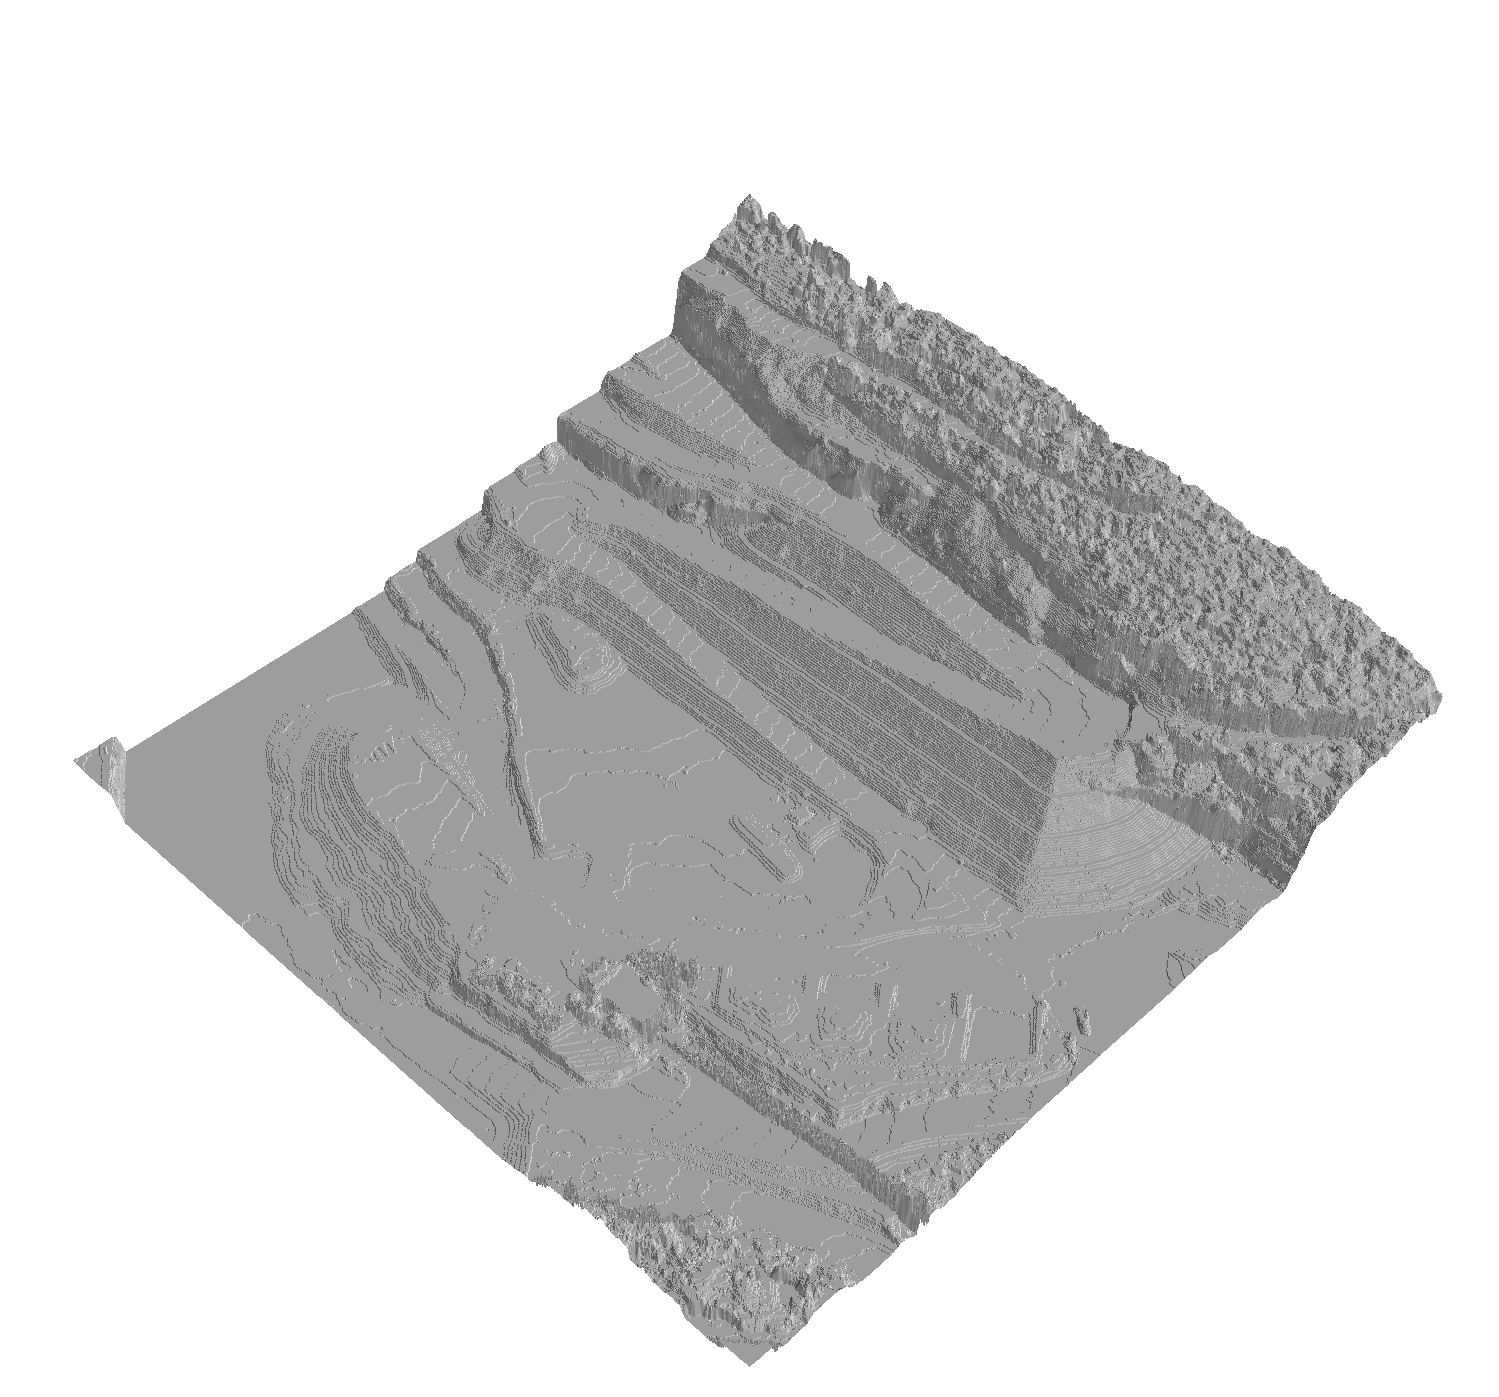
\includegraphics[width=\textwidth]{../img/hm3d/querry-big-10.png}
        \caption{Quarry}
    \end{subfigure}
    \begin{subfigure}[b]{0.45\textwidth}
        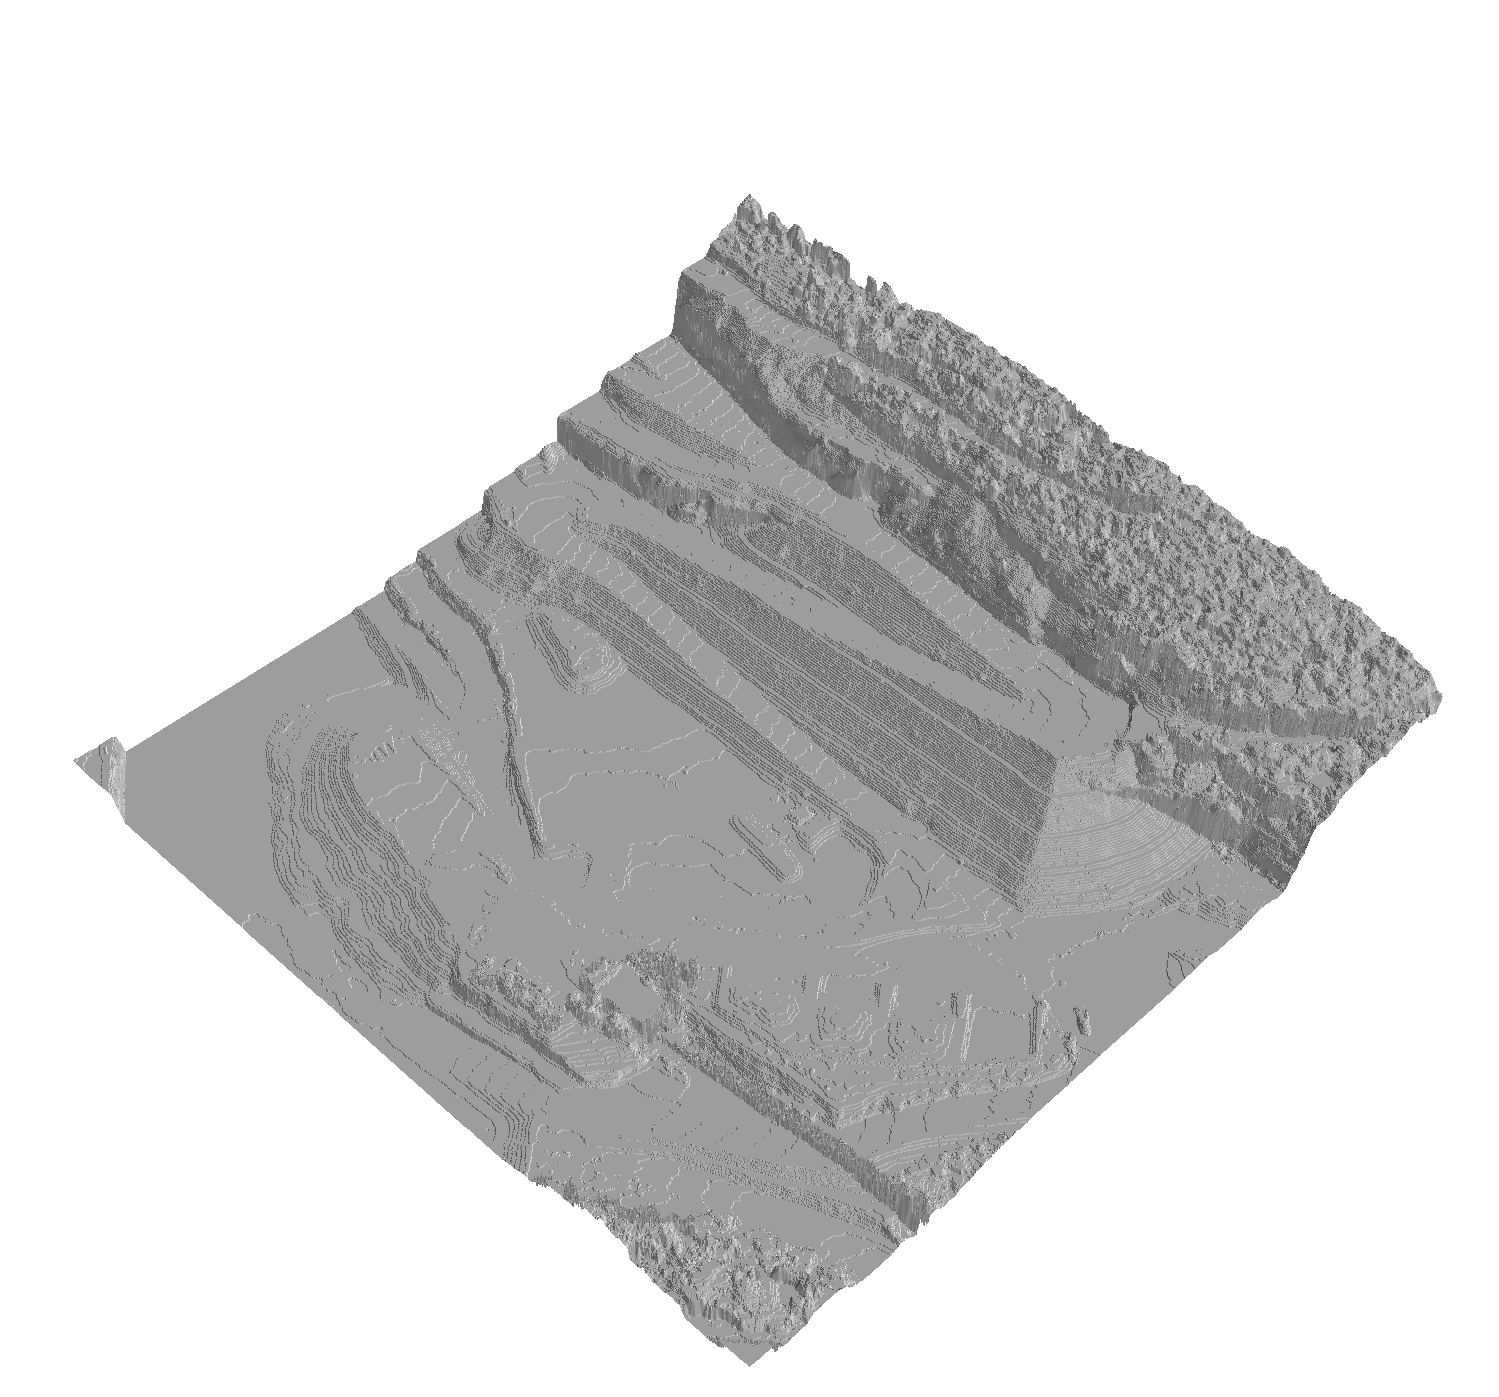
\includegraphics[width=\textwidth]{../img/hm3d/querry-big-10.png}
        \caption{Quarry}
    \end{subfigure}  
\caption{Real world maps obtained from \href{https://www.sensefly.com/education/datasets/}{sensefly}'s dataset..}  
\end{figure}

Quarry is used as test set to evaluate the model performance.
\subsubsection{Simulation}
To collect \emph{Krock}'s interaction with the environment, we spawn the robot on the ground and let it move forward for $t$ seconds. We repeat this process $n$ times per each map.
    Unfortunately, spawning the robot is not a trivial task. In certain maps, for instance, \emph{bars1}, a map with tons of walls, we must avoid spawning Krock on an obstacle otherwise the run will be ruined by \emph{Krock} getting stuck at the beginning introducing noise in the dataset. To solve the problem, we defined two spawn strategies, a random spawn and a flat ground spawn strategy. The first one is used in most of the maps without big obstacles such as \emph{slope\_rocks}. This stragety just spawn the robot on random position and rotation. 
    While, the flat ground strategy isfirst selects suitable spawn positions by using a sliding window on the heightmap of size equal Krock's footprint and check if the mean pixel value is lower than a small threshold. If so, we store the center coordinates of the patch as a candidate spawing point. Intuitively, if a patch is flat then its mean value will be close to zero.
Since there may be more flat spawing positions than simulations needed, we have to reduce the size of the candidate points. To maintaing the correct distribution on the map to avoid spawing the robot always in the same cloud of points, we used K-Means with $k$ clusters where $k$ is equal to the number of simulations we wish to run. By clustering, we guarantee to cover all region of the map removing any bias. The following picture shows this strategy on \emph{bars1}. 
\begin{figure}[H]
    \begin{subfigure}[b]{0.45\textwidth}
        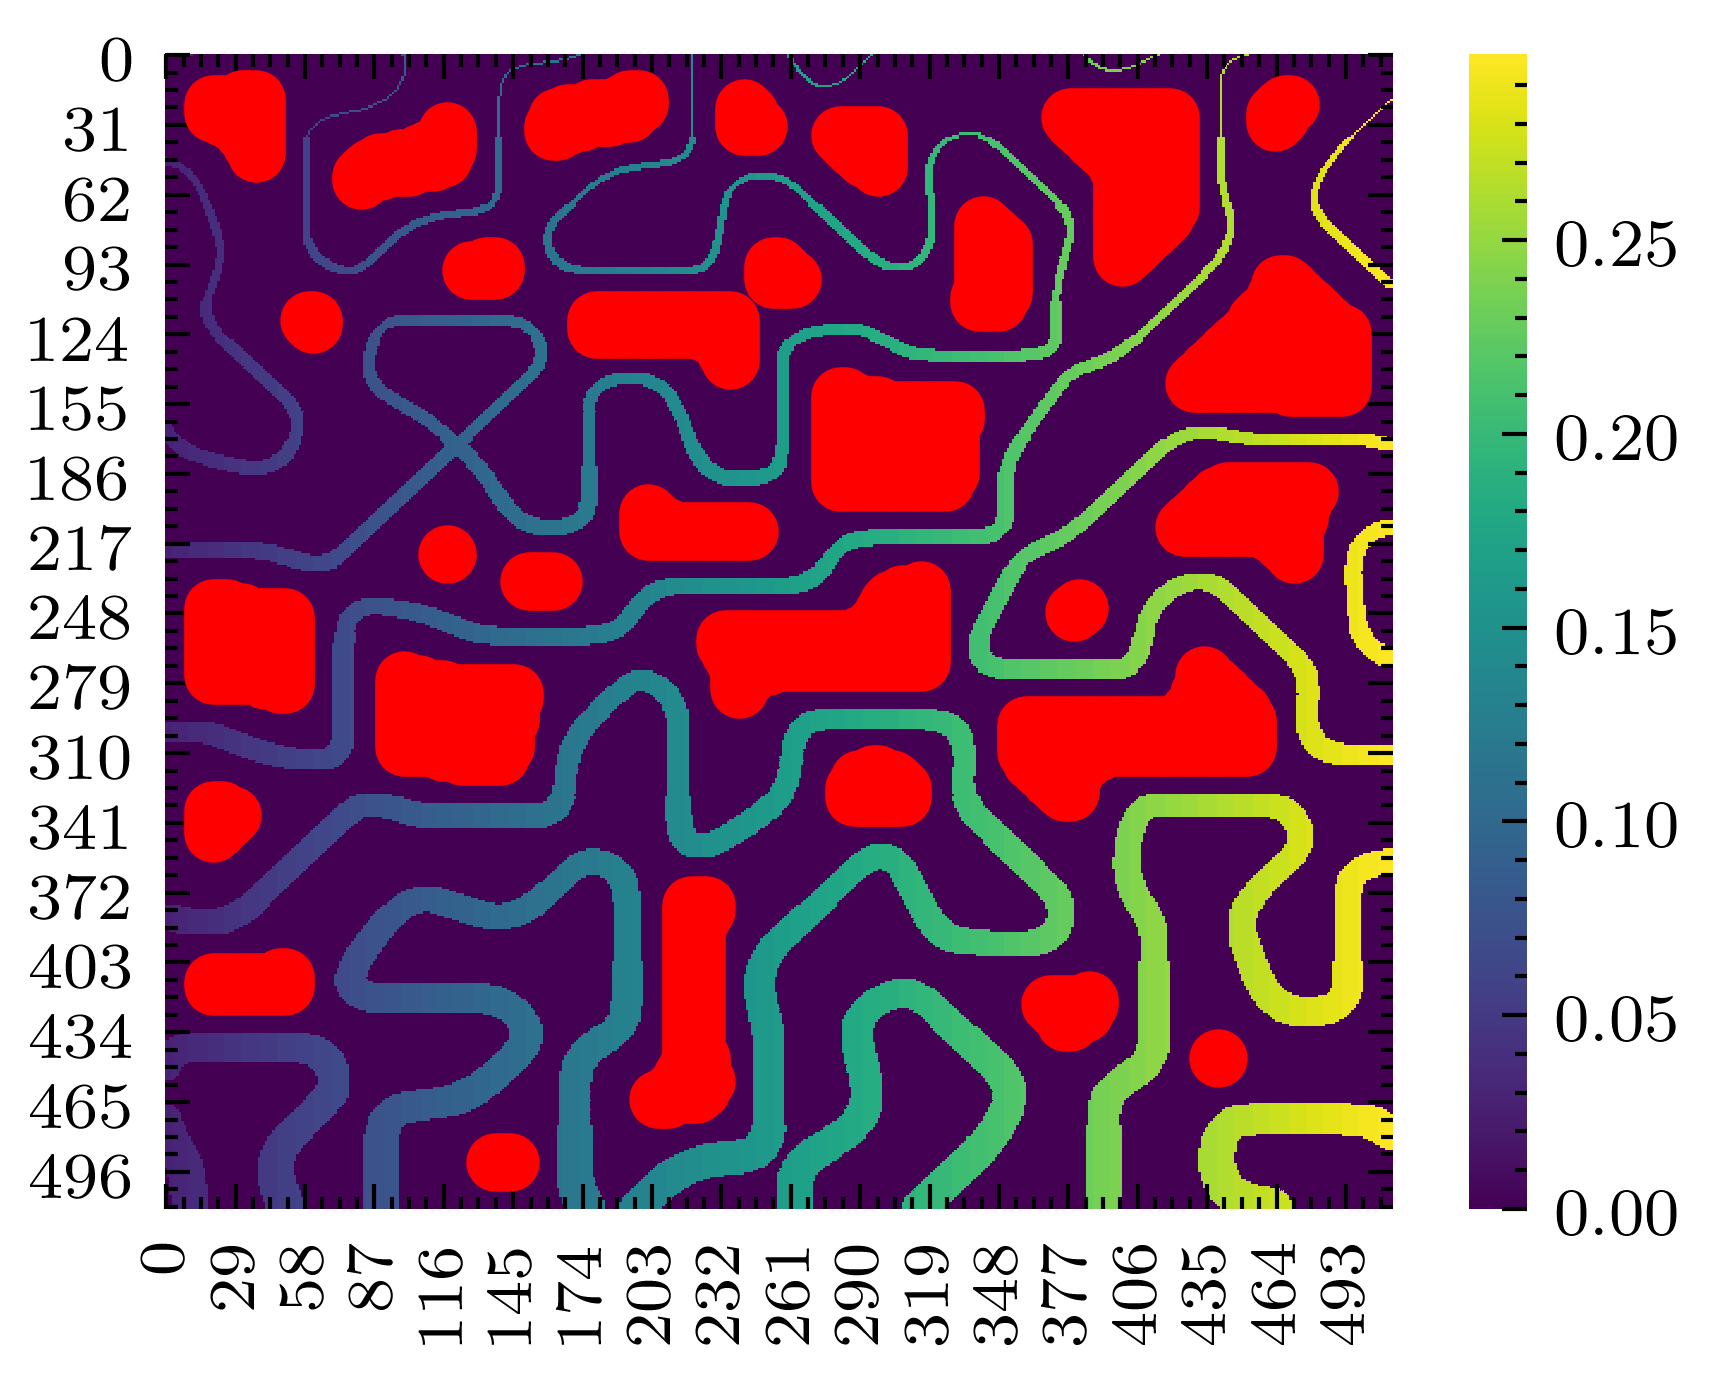
\includegraphics[width=\textwidth]{../img/3/spawn/flat-spawn-10.png}
        \caption{Flat regions}
    \end{subfigure}
    \begin{subfigure}[b]{0.45\textwidth}
        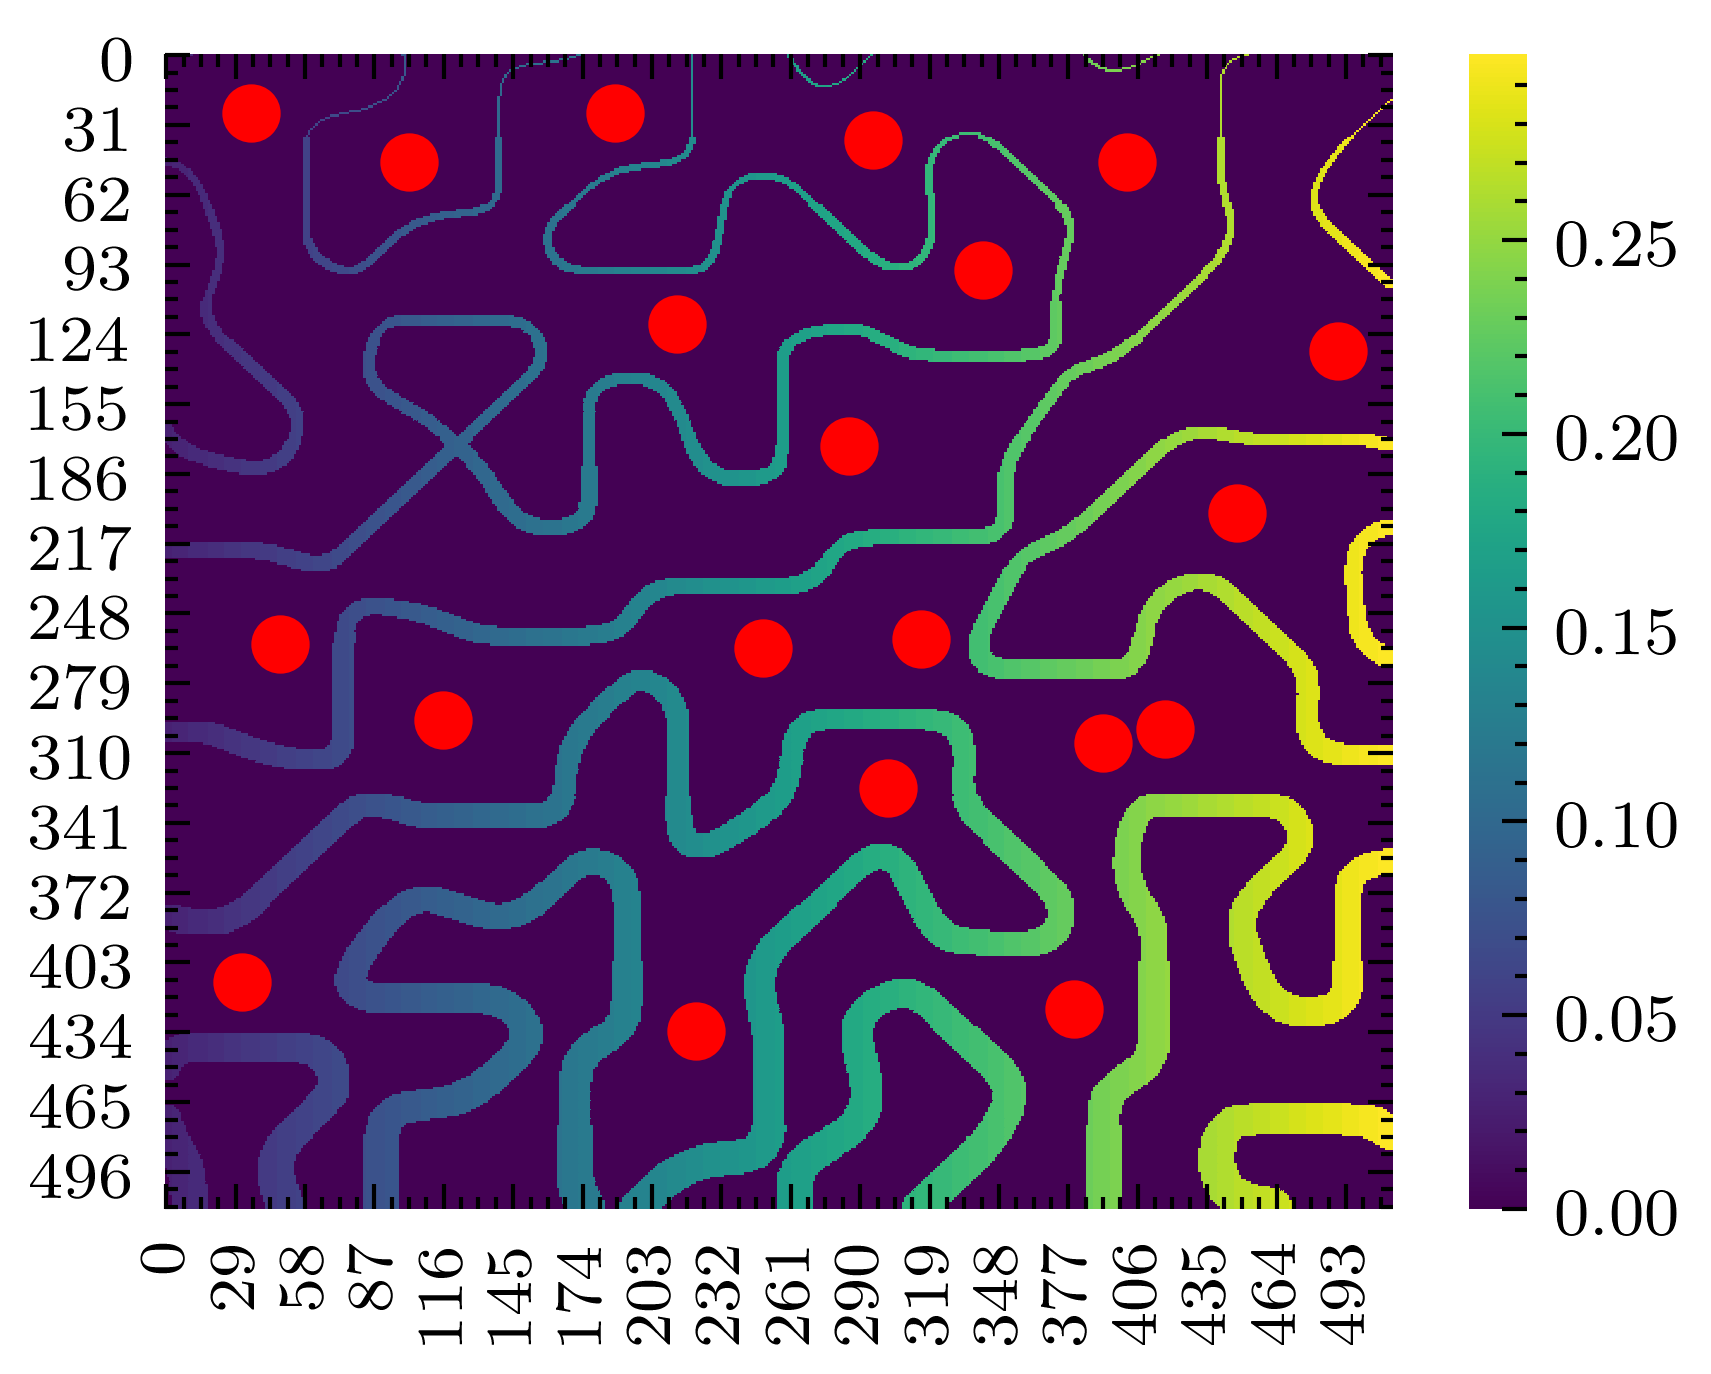
\includegraphics[width=\textwidth]{../img/3/spawn/spawn-10.png}
        \caption{K-Means with $k=20$}
    \end{subfigure}  
\label{fig: spawn-strat}
\caption{Examples of the spawning selection process (marked as red blobs) for the map \emph{bars1} }   
\end{figure}
The following table shows the maps configuration used in the simulator.
\begin{table}[H]
    \centering
    \ra{1.2}
    
    \begin{tabular}[]{@{}llccccc@{}}
      \toprule
      & Map & Height(m) & Spawn & Texture & Simulations & max time(s) \\ 
      \hline
      &\multirow{3}{*}{\emph{bumps0}} & \multirow{3}{*}{2} & \multirow{3}{*}{random} &- & \multirow{3}{*}{50} & \multirow{3}{*}{10} \\
      &&&& rocks1 &  &  \\ 
      &&&& rocks2 &  &  \\ 
      \hline
      &\multirow{3}{*}{\emph{bumps1}} & \multirow{3}{*}{1} & \multirow{3}{*}{random}& - & \multirow{3}{*}{50} & \multirow{3}{*}{10} \\
      &&&& rocks1 &  &  \\ 
      &&&& rocks2 &  &  \\ 
      \hline
      &\multirow{4}{*}{\emph{bumps2}} & \multirow{3}{*}{1} & \multirow{4}{*}{random} &- & \multirow{3}{*}{50} & \multirow{4}{*}{10} \\
      &&&& rocks1 &  &  \\ 
      &&&& rocks2 &  &  \\ 
      && 2 && - &  &  \\ 
      \hline
      &\multirow{3}{*}{\emph{bumps3}} & \multirow{3}{*}{1}& \multirow{3}{*}{random} & - & \multirow{4}{*}{50} & \multirow{3}{*}{10} \\
      &&&& rocks1 &  &  \\ 
      &&&& rocks2 &  &  \\ 
      \hline
      &\emph{steps1} & 1 &random & - & 50 & 10 \\
      \hline
      &\emph{steps2} & 1 &flat & - & 50  &  10\\
      \hline
      &\emph{steps3} & 1 &random & - & 50  &  10\\
      \hline
      &\emph{rails1} & 1 & flat & - & 50 & 20 \\
      \hline
      &\emph{rails2} & 1 && flat & - & 10 \\
      \hline
      &\emph{rails3} & 1 &&  flat&  - & 10 \\
      \hline
      &\multirow{2}{*}{\emph{bars1}} & 1 & \multirow{2}{*}{flat} & - & \multirow{2}{*}{50} & \multirow{2}{*}{10} \\
      && 2 &  & - &  &  \\
      \hline
      &\emph{bars3} & 1 & flat  & - &  &  \\
      \hline
      &\multirow{2}{*}{\emph{ramp0}} & \multirow{2}{*}{1} & \multirow{2}{*}{random} & rocks1 & 50 & \multirow{2}{*}{10} \\
      &&&& rocks2 & 50 &  \\
      \hline
      &\multirow{3}{*}{\emph{ramp1}} & 3 & \multirow{3}{*}{random} & \multirow{3}{*}{-} & \multirow{3}{*}{50} & \multirow{3}{*}{10} \\
      && 4 &&&& \\
      && 5 &&&& \\
      \hline 
      &\multirow{3}{*}{\emph{slope\_rocks1}} & 3 & \multirow{3}{*}{random} & \multirow{3}{*}{-} & \multirow{3}{*}{50} & \multirow{3}{*}{10} \\
      && 4 &&&& \\
      && 5 &&&& \\
      \hline
      &\emph{holes1} & 1 &random & - & 50 & 10 \\
      \hline
      &\emph{quarry} & 10 &random & - & 50 & 10 \\
      &&& Total: 1600 \\ 
      \bottomrule   
    \end{tabular}
    \label{table: maps}
    \caption{Maps configuration used in the simulator.}
  \end{table}

\subsection{Postprocessing}
After the run Krock on each map, we need to extract the patches for each stored pose $p_i$ and compute the advancement for a given time window, $\Delta t$.
\subsubsection{Parse simulation data}
First, we turn each \emph{.bag} file into a pandas dataframe and cache them into \emph{.csv} files. We used \href{https://github.com/aktaylor08/RosbagPandas}{\texttt{rosbag\_pandas}}, an open source library we ported to python3, to perform the conversion.
Then, we load the dataframes with the respective heightmaps and start the data cleaning process. We remove the rows corresponding tp the first second of the simulation time to account for the robot spawning time. Then we eliminate all the entries where the \emph{Krock} pose was near the edges of a map, we used a threshold of $22$ pixels since we notice  \emph{Krock} getting stuck in the borders of the terrain during a simulation. 
After cleaning the data, we convert \emph{Krock}quaternion rotation to Euler notation using the \href{https://duckduckgo.com/?q=ros+tf&atb=v154-1__&ia=web}{\texttt{tf}} package from ROS. Then, we extract the $\sin$ and $\cos$ from the Euler orientation last component and store them in a column.
Before caching again the resulting dataframes into \emph{.csv} files, we convert the robot's position into heightmap's coordinates that are used later to crop the correct region of the map.

To compute the robot's advancement in a time window $\Delta t$ we look for each stored pose ,$p_t$, in the future, $p_{t + \Delta t}$, and see how far it went. This is describe by the following equation: 
\todo[inline]{ask omar}
The correct value of $\Delta t$ is crucial. We want a time window small enough to avoid smoothing to much the advancement and making obstacle traversale, and big enough to include the full legs motion. We empirically set $\Delta t = 2$ since it allows Krock to move both its legs and does not flat the advancement too much. 
\subsubsection{Extract patches}
Each patch must contain both Krock's footprint, to include the situations where the obstacle is under the robot, and certain amount of ground region in front of it. Intuitively, we want to include in each patch the correct amount of future informations according to the selected time window. Thus, we should add the maximum possible ground that Krock could traverse. 

To find out the correct value, we must compute the maximum advancement on a flat ground for the $\Delta t$ and use it to calculate the final size of the patch. We compute it by running some simulations of \emph{Krock} on flat ground and averaging the advancement getting a value of $71$cm in our $\Delta t = 2$s.

Each patch must include Krock's footprint and the maximum possible distance it can travel is a $\Delta t$. So, since Krock's pose was stored from IMU located in the juncture between the head and the legs, we have to crop from behind its length, $85$cm minus the offset between the IMU and the head, $14$cm. Then, we have to take $71$cm, the maximum advancement with a $\Delta t = 2$s plus the removed offset. The following figure visualizes the patch extraction process. 
\begin{figure}[H]
    \centering
    \begin{subfigure}[b]{0.66\textwidth}
        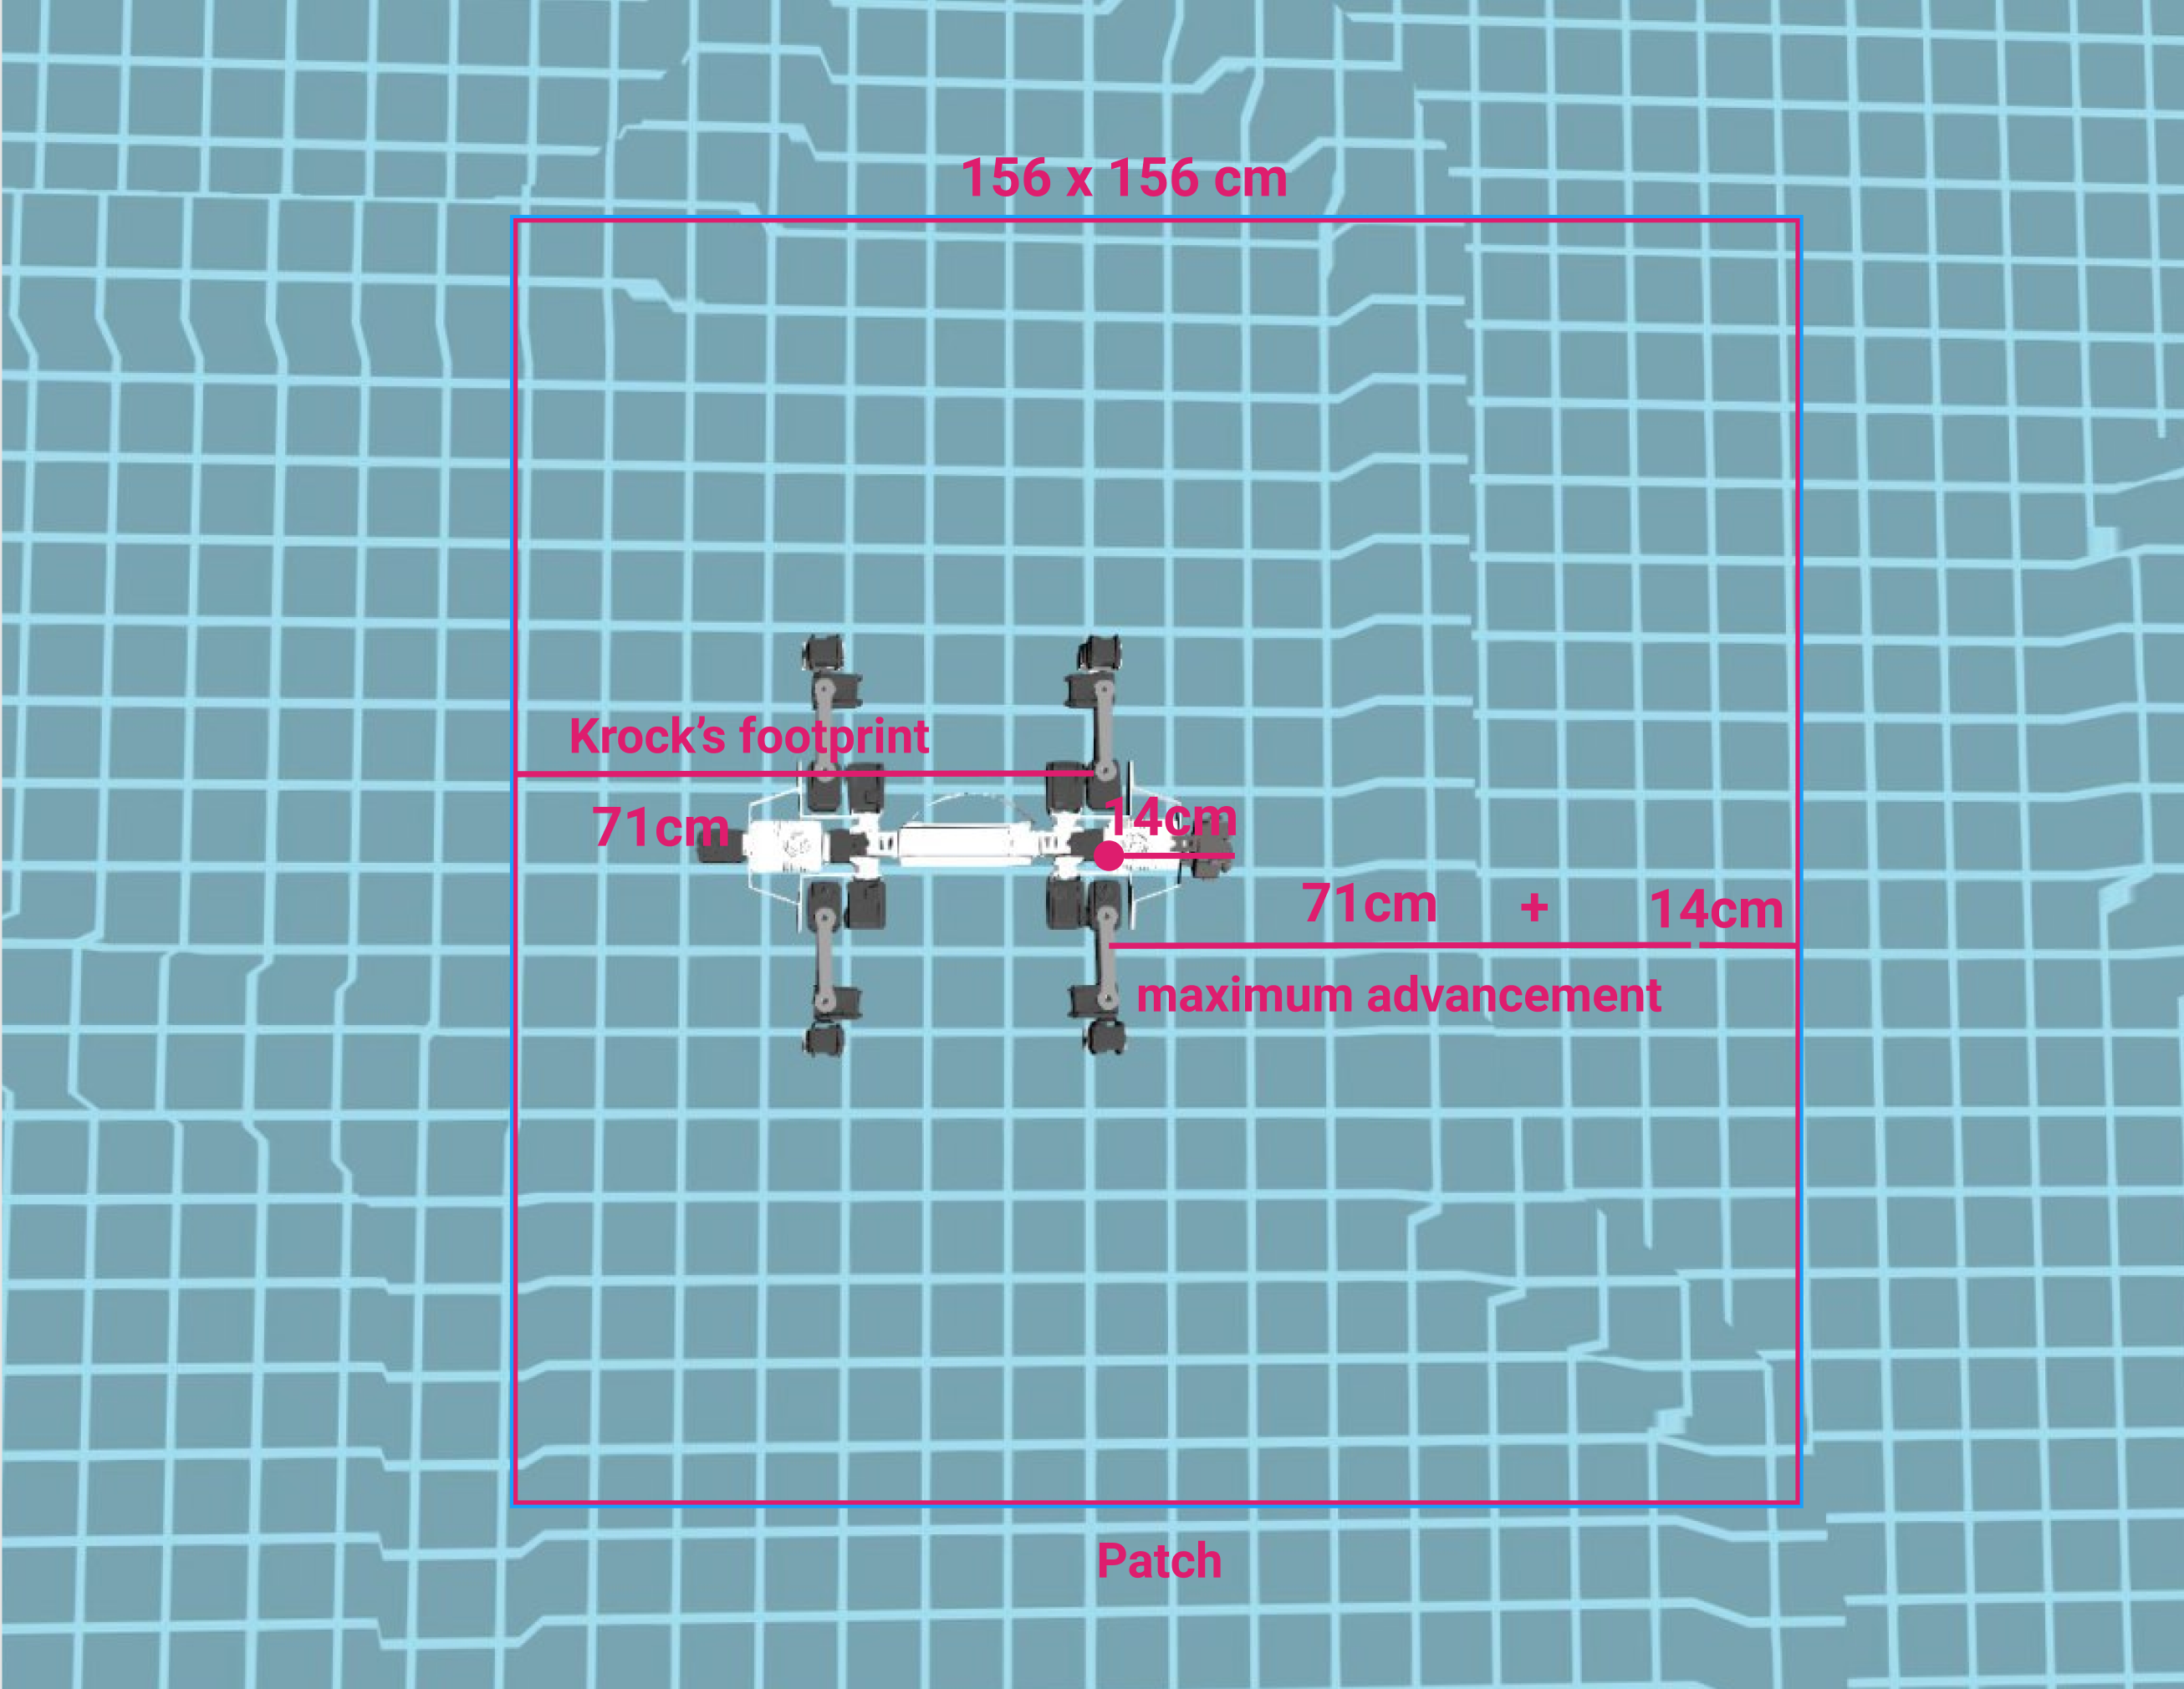
\includegraphics[width=\textwidth]{../img/3/crop/crop.png}
        \caption{Robot in the simulator.}
    \end{subfigure}
    \begin{subfigure}[b]{0.45\textwidth}
        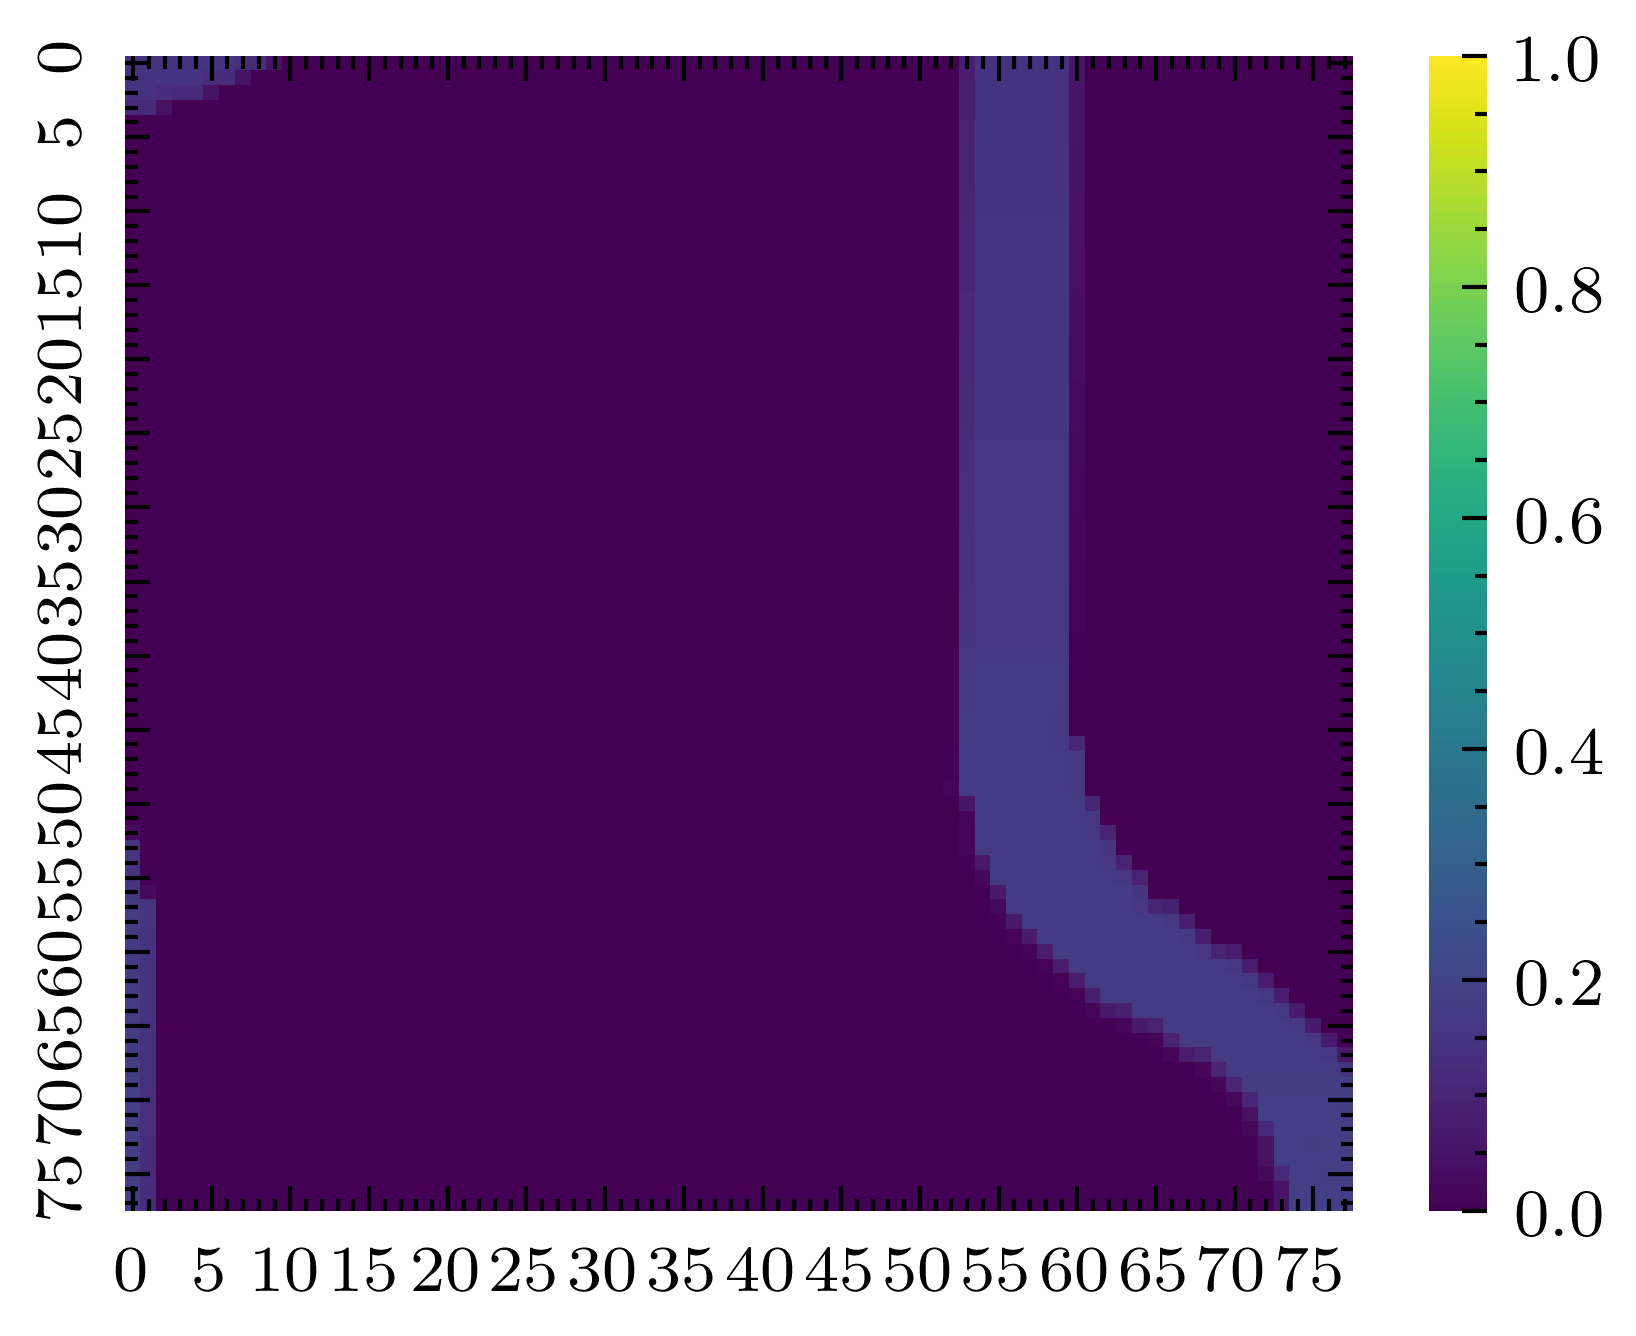
\includegraphics[width=\textwidth]{../img/3/crop/test-1-2d.png}
        \caption{Cropped patch in 2d.}
    \end{subfigure}
    \begin{subfigure}[b]{0.45\textwidth}
        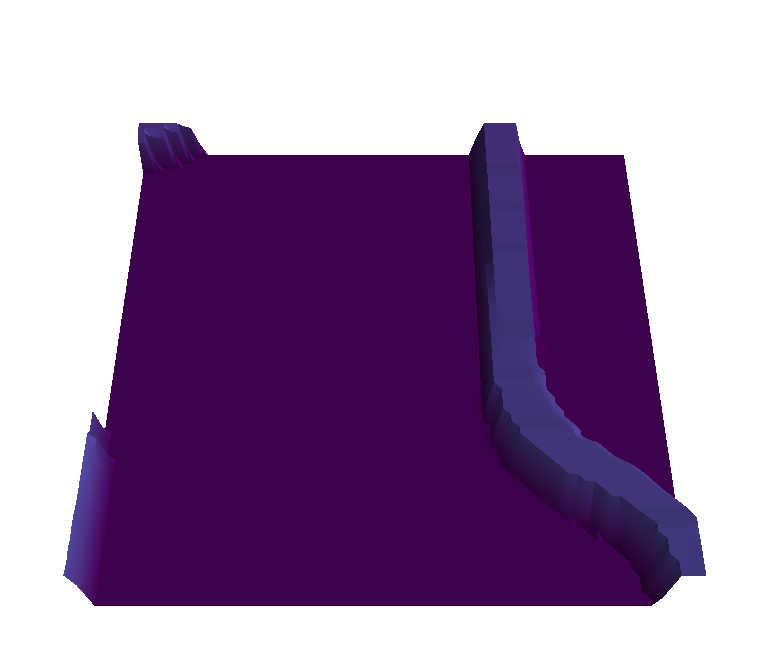
\includegraphics[width=\textwidth]{../img/3/crop/test-1-3d.png}
        \caption{Cropped patch in 3d.}
    \end{subfigure}
\caption{Patch extraction process for $\Delta t = 2$s.}   
\end{figure}
Lastly, we create a final dataframe containing the map coordinates, the advancement, and the patches paths for each simulation and store them to disk as \emph{.csv} files. 

The whole pipeline takes less than one hour to run the first time with 16 threads, and, once it is cached, less than fifteen minutes to extract all the patches. In total, we created almost half a milion images.

Once we extract the patches, we can always re-compute the advancement without re-running the whole pipeline. The next figure show the proposed pipeline.
\begin{figure}[H] 
\centering
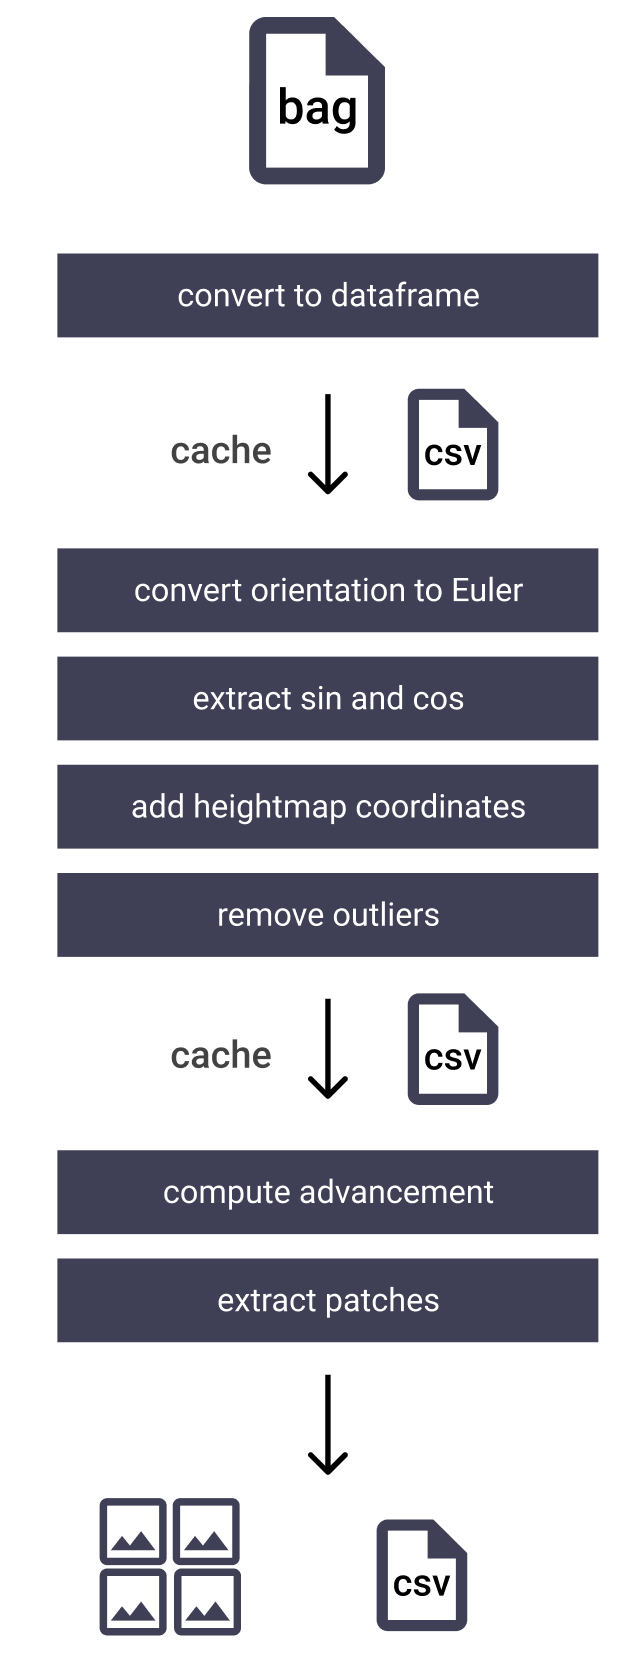
\includegraphics[width=0.4\textwidth]{../img/postprocessing-pipeline.png}
\caption{Postprocessing Pipeline flow graph, starting from the top.}
\label{fig: postprocessing-pipeline}
\end{figure}
The following figure shows the mean advancement across all the maps used to train the model in a range of $\pm 0.71$cm, the maximum advancment the used time window, $\Delta t = 2$s.
\begin{figure}[H]
    \centering
    \includegraphics[width=\linewidth]{../img/datasets/box_for_each_map.png}
    \caption{Advancement on each map with a $\Delta t = 2$s in ascendent order.}
\end{figure}
To give the reader a better idea of how the patches looks like, the next figures shows the 3d render of some patches extracted form \emph{Quarry} ordered by advancement.
\begin{figure}[H]
    \centering
    \begin{subfigure}[b]{0.19\textwidth}
    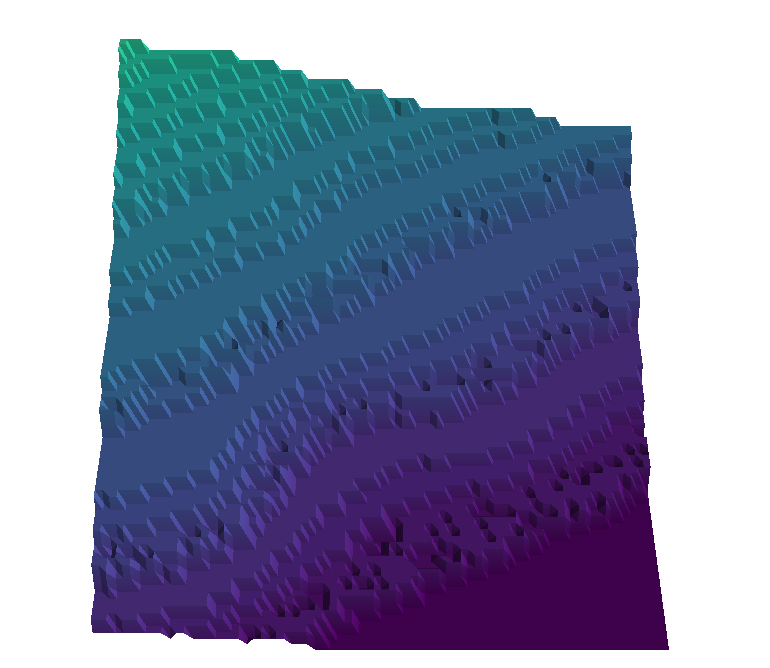
\includegraphics[width=\linewidth]{../img/5/quarry/all/best/35-patch-3d-majavi-colormap-0.png}
    \caption{$35$cm}
    \end{subfigure}
    \begin{subfigure}[b]{0.19\textwidth}
    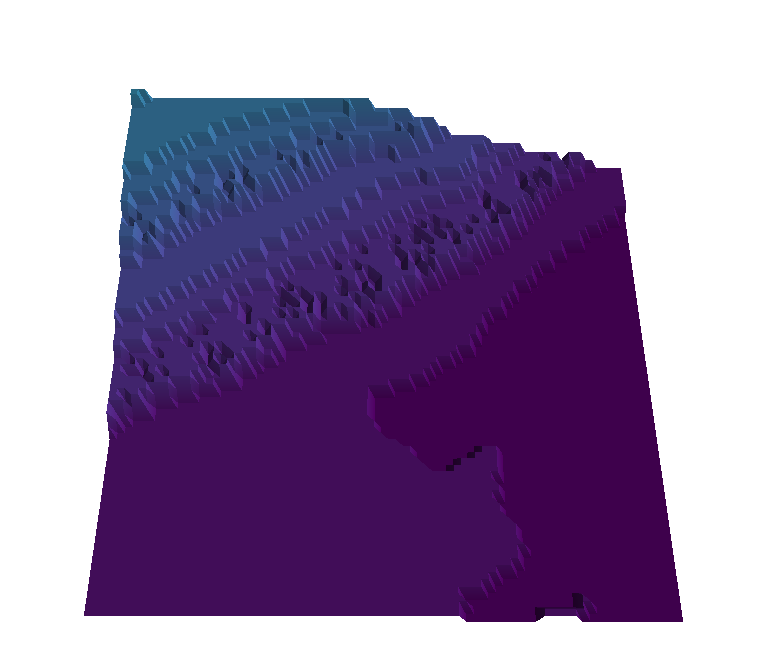
\includegraphics[width=\linewidth]{../img/5/quarry/all/best/38-patch-3d-majavi-colormap-1.png}
    \caption{$38$cm}
    \end{subfigure}
    \begin{subfigure}[b]{0.19\textwidth}
    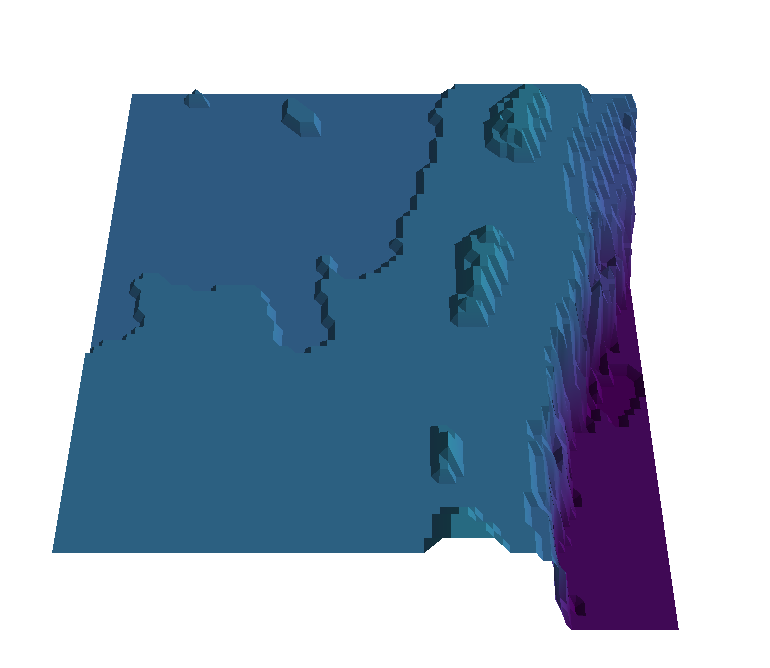
\includegraphics[width=\linewidth]{../img/5/quarry/all/best/44-patch-3d-majavi-colormap-2.png}
    \caption{$44$cm}
    \end{subfigure}
    \begin{subfigure}[b]{0.19\textwidth}
    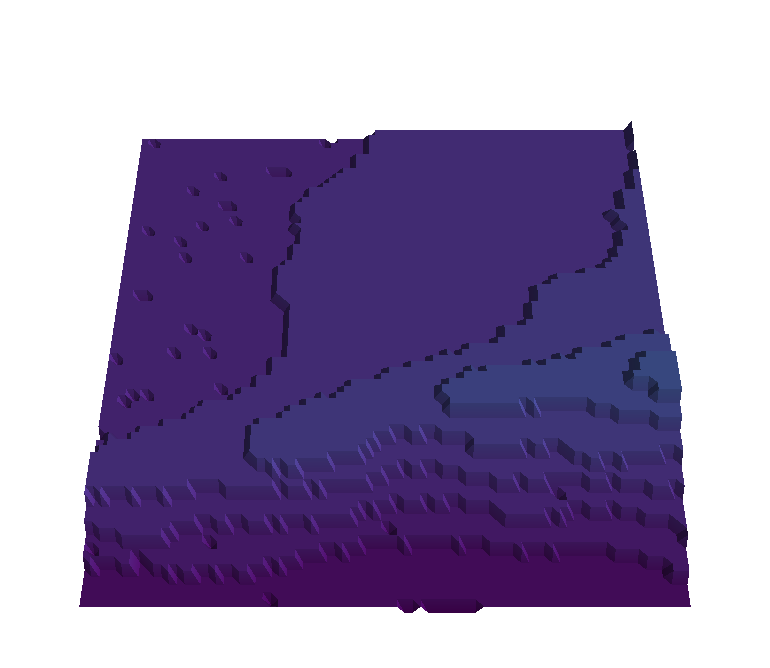
\includegraphics[width=\linewidth]{../img/5/quarry/all/best/45-patch-3d-majavi-colormap-3.png}
    \caption{$45$cm}
    \end{subfigure}
    \begin{subfigure}[b]{0.19\textwidth}
    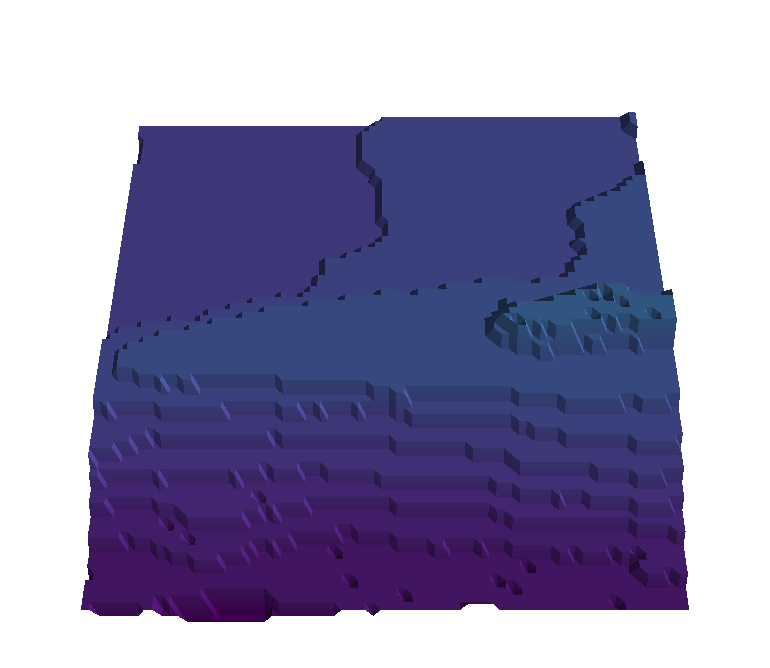
\includegraphics[width=\linewidth]{../img/5/quarry/all/best/49-patch-3d-majavi-colormap-4.png}
    \caption{$49$cm}
    \end{subfigure}
    \begin{subfigure}[b]{0.19\textwidth}
    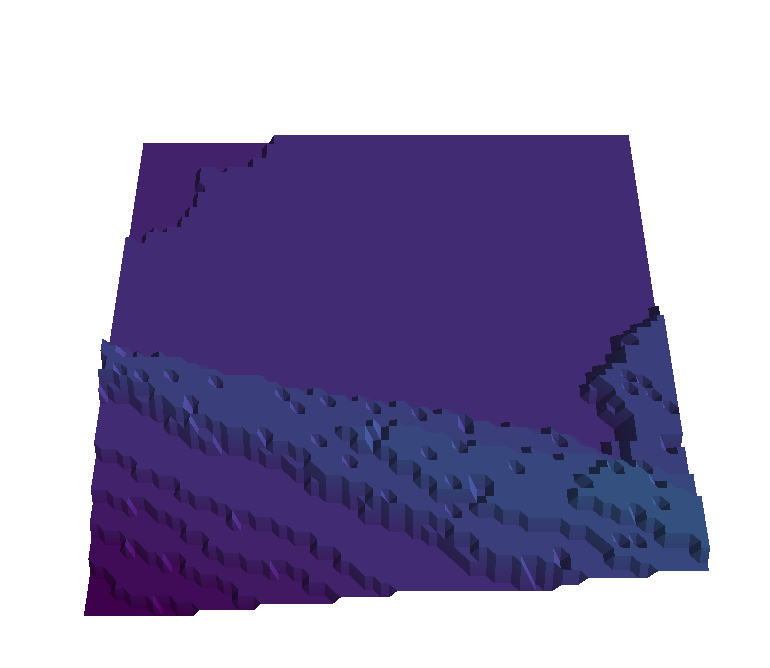
\includegraphics[width=\linewidth]{../img/5/quarry/all/best/51-patch-3d-majavi-colormap-5.png}
    \caption{$51$cm}
    \end{subfigure}
    \begin{subfigure}[b]{0.19\textwidth}
    
\includegraphics[width=\linewidth]{../img/5/quarry/all/best/65-patch-3d-majavi-colormap-6.png}
    \caption{$65$cm}
    \end{subfigure}
    \begin{subfigure}[b]{0.19\textwidth}
    
\includegraphics[width=\linewidth]{../img/5/quarry/all/best/67-patch-3d-majavi-colormap-7.png}
    \caption{$67$cm}
    \end{subfigure}
    \begin{subfigure}[b]{0.19\textwidth}
    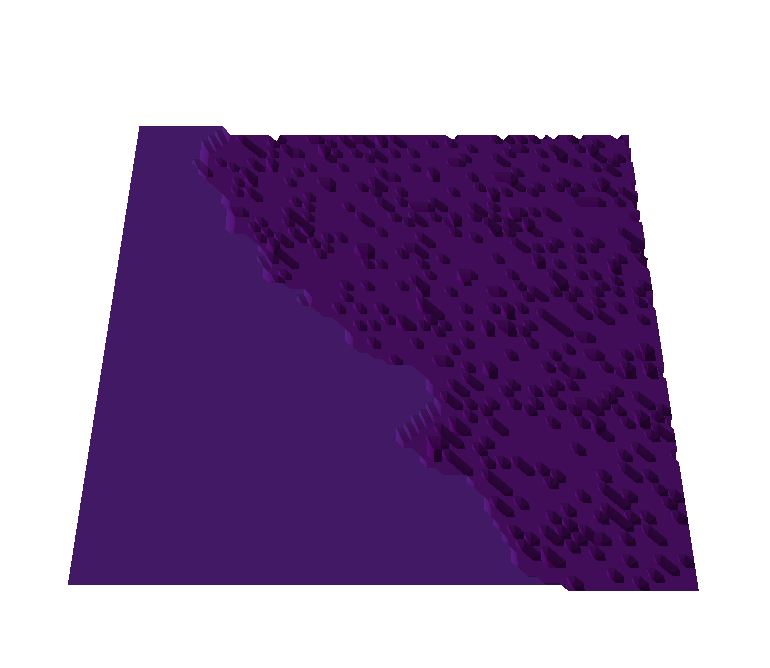
\includegraphics[width=\linewidth]{../img/5/quarry/all/best/67-patch-3d-majavi-colormap-8.png}
    \caption{$67$cm}
    \end{subfigure}
    \begin{subfigure}[b]{0.19\textwidth}
    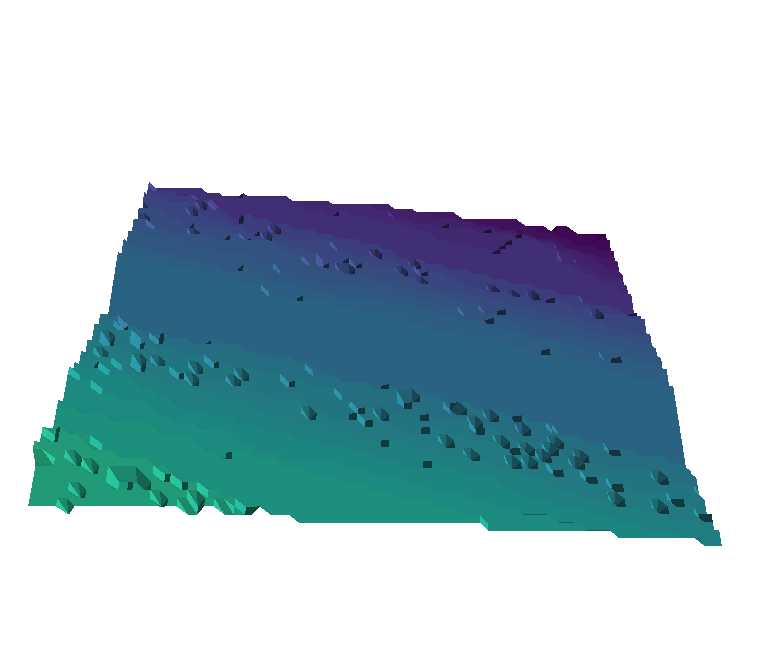
\includegraphics[width=\linewidth]{../img/5/quarry/all/best/72-patch-3d-majavi-colormap-9.png}
    \caption{$72$cm}
    \end{subfigure}
    \caption{Patches with high advancement \emph{Quarry} using a $\Delta t = 2$s.}
\end{figure}
    \begin{figure}[H]
        \centering
        \begin{subfigure}[b]{0.19\textwidth}
        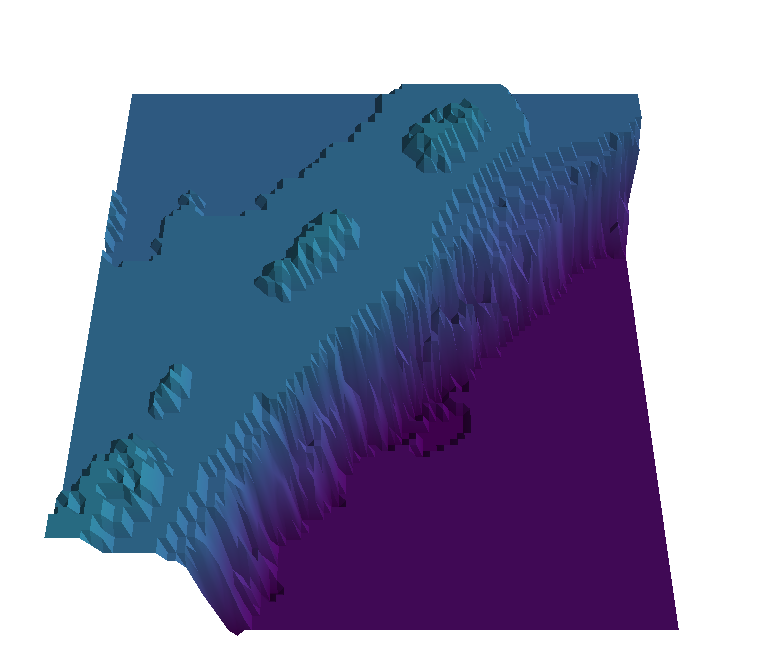
\includegraphics[width=\linewidth]{../img/5/quarry/all/worst/-8-patch-3d-majavi-colormap-0.png}
        \caption{$-8$cm}
        \end{subfigure}
        \begin{subfigure}[b]{0.19\textwidth}
        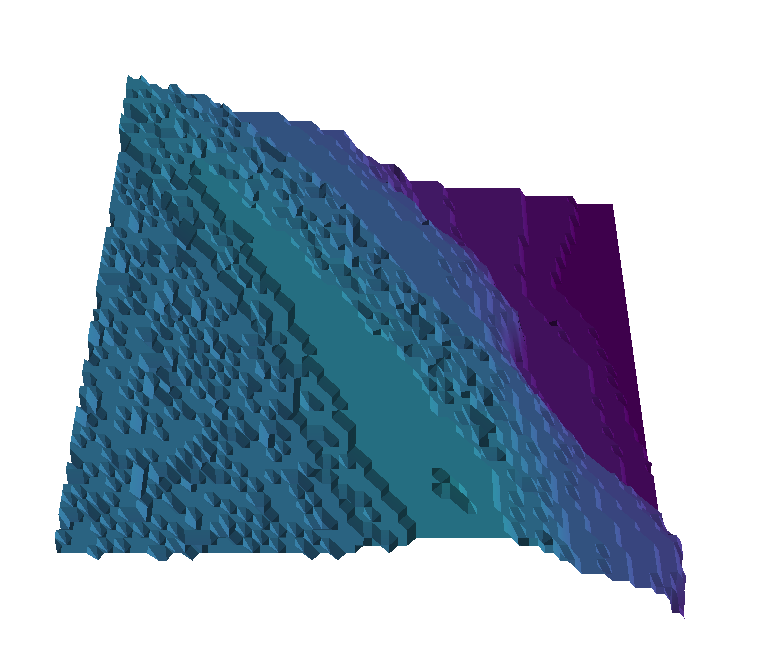
\includegraphics[width=\linewidth]{../img/5/quarry/all/worst/00-patch-3d-majavi-colormap-1.png}
        \caption{$00$cm}
        \end{subfigure}
        \begin{subfigure}[b]{0.19\textwidth}
        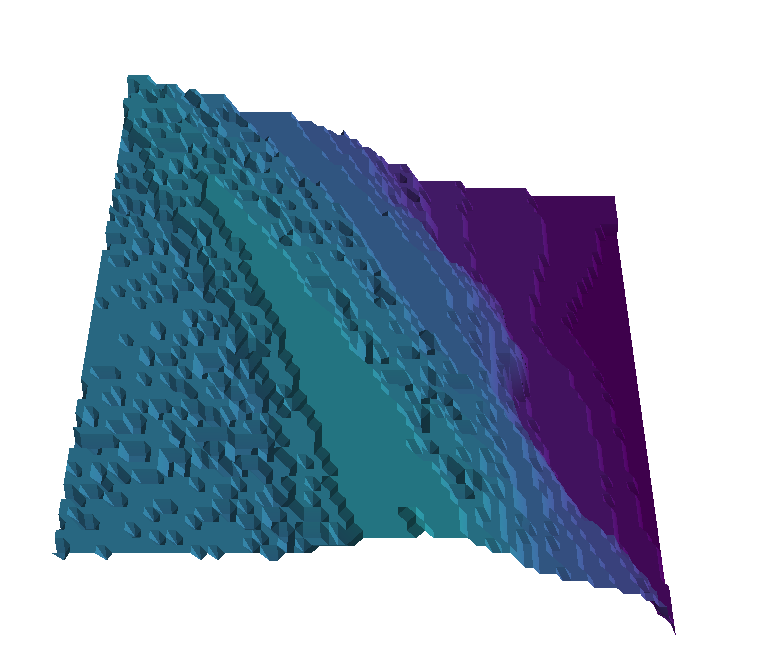
\includegraphics[width=\linewidth]{../img/5/quarry/all/worst/01-patch-3d-majavi-colormap-2.png}
        \caption{$01$cm}
        \end{subfigure}
        \begin{subfigure}[b]{0.19\textwidth}
        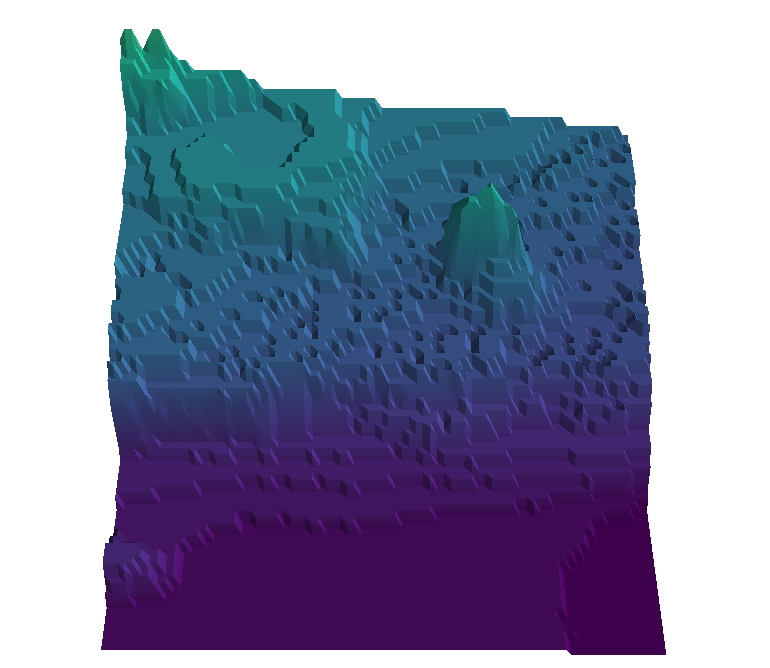
\includegraphics[width=\linewidth]{../img/5/quarry/all/worst/01-patch-3d-majavi-colormap-3.png}
        \caption{$01$cm}
        \end{subfigure}
        \begin{subfigure}[b]{0.19\textwidth}
        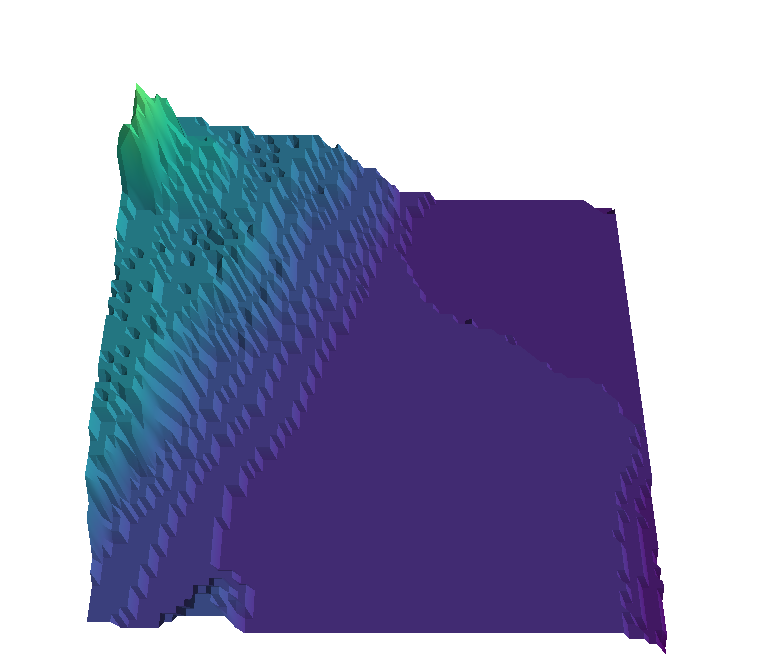
\includegraphics[width=\linewidth]{../img/5/quarry/all/worst/02-patch-3d-majavi-colormap-4.png}
        \caption{$02$cm}
        \end{subfigure}
        \begin{subfigure}[b]{0.19\textwidth}
        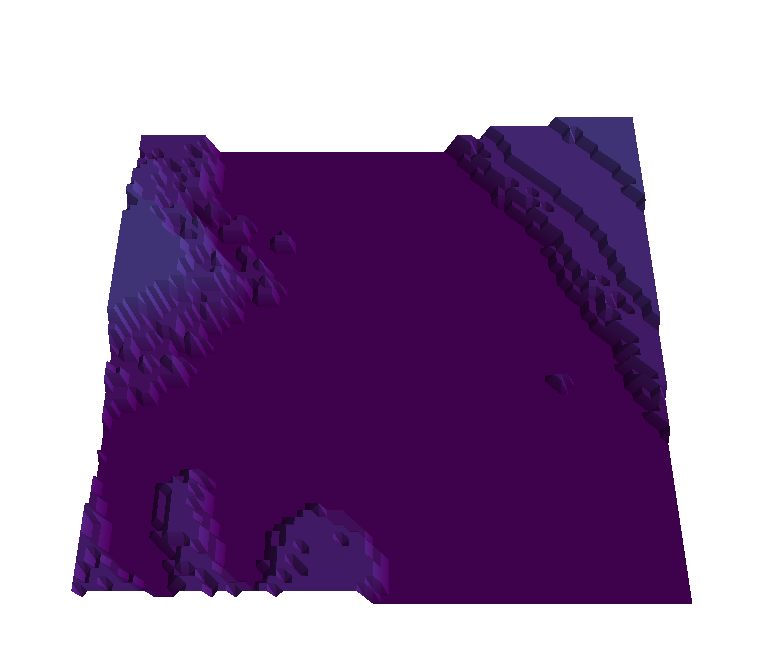
\includegraphics[width=\linewidth]{../img/5/quarry/all/worst/03-patch-3d-majavi-colormap-5.png}
        \caption{$03$cm}
        \end{subfigure}
        \begin{subfigure}[b]{0.19\textwidth}
        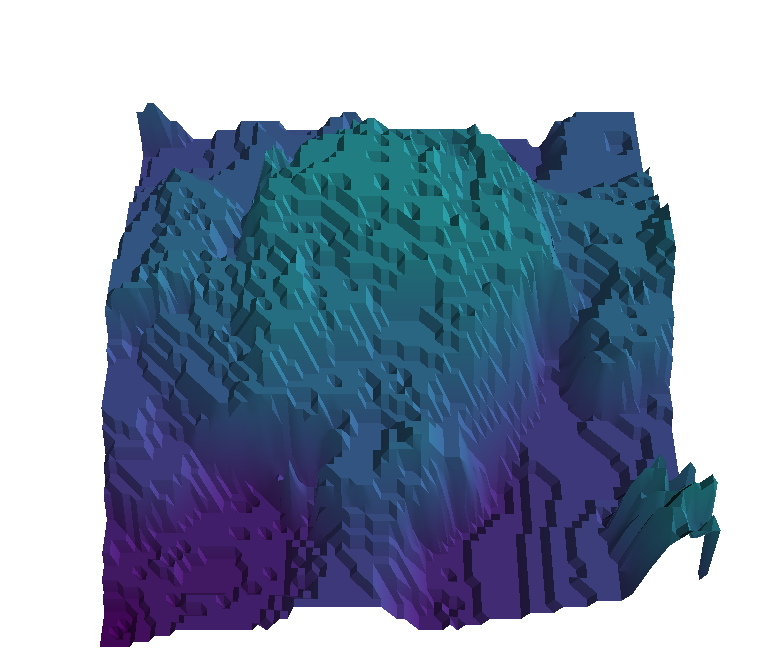
\includegraphics[width=\linewidth]{../img/5/quarry/all/worst/06-patch-3d-majavi-colormap-6.png}
        \caption{$06$cm}
        \end{subfigure}
        \begin{subfigure}[b]{0.19\textwidth}
        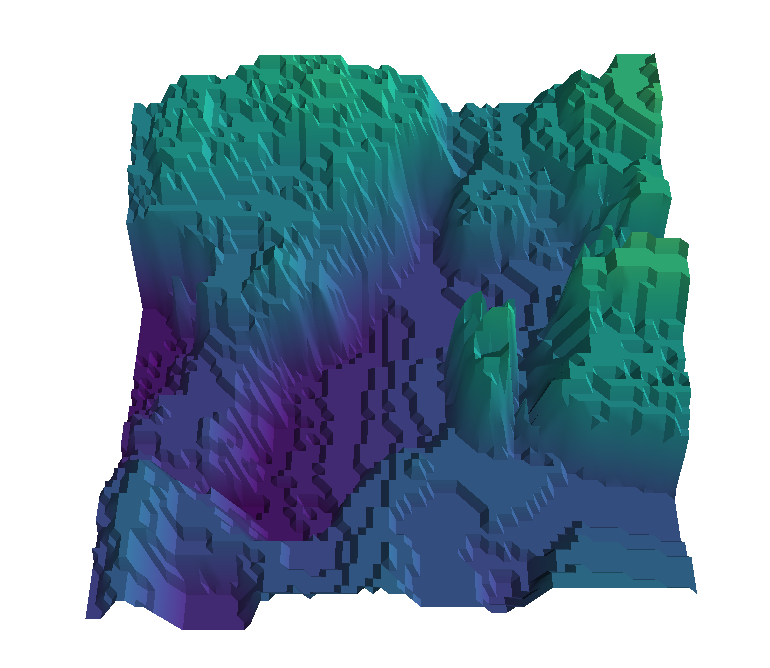
\includegraphics[width=\linewidth]{../img/5/quarry/all/worst/06-patch-3d-majavi-colormap-7.png}
        \caption{$06$cm}
        \end{subfigure}
        \begin{subfigure}[b]{0.19\textwidth}
        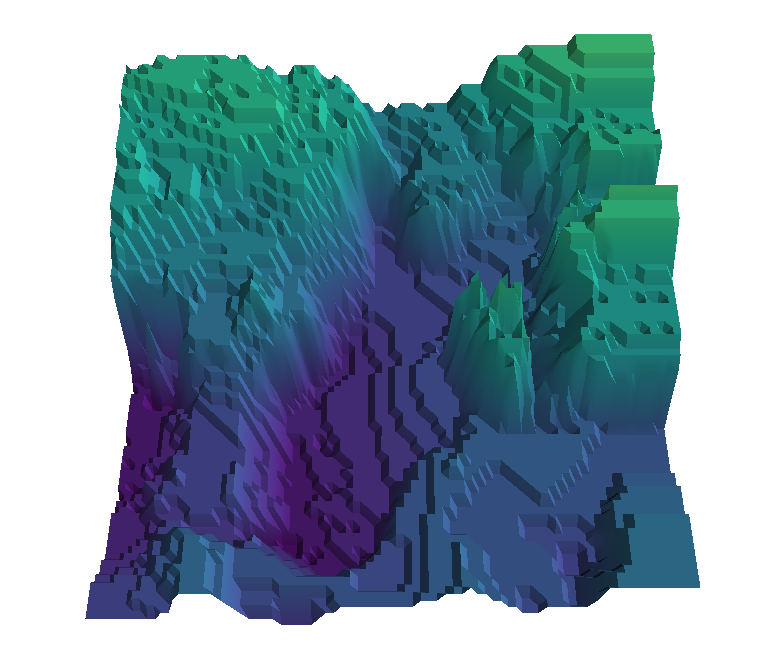
\includegraphics[width=\linewidth]{../img/5/quarry/all/worst/10-patch-3d-majavi-colormap-8.png}
        \caption{$10$cm}
        \end{subfigure}
        \begin{subfigure}[b]{0.19\textwidth}
        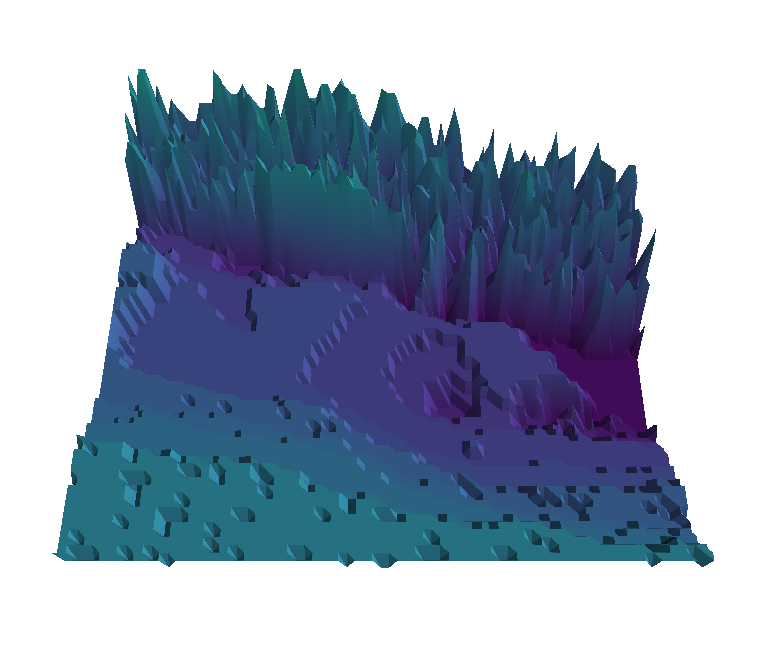
\includegraphics[width=\linewidth]{../img/5/quarry/all/worst/18-patch-3d-majavi-colormap-9.png}
        \caption{$18$cm}
        \end{subfigure}
        \caption{Patches with low advancement \emph{Quarry} a $\Delta t = 2$s.}
    \end{figure}
Corretly, the patches with a lower advancement values have some ostacle in front of the robot, while the other set of inputs are almost flat.

All the handles used to postprocess the data are available as a python \href{https://github.com/FrancescoSaverioZuppichini/Master-Thesis/tree/master/core/utilities/postprocessing/handlers}{package}. Also, we create an easy to use API called \href{https://github.com/FrancescoSaverioZuppichini/Master-Thesis/tree/master/core/utilities/pipeline}{\texttt{pipeline}} to define a cascade stream of function that is applied one after the other using a multi-thread queue to speed-up the process.

\subsubsection{Label the Patches}
To decide whether a patch is traversable or not traversable we need to decide a \emph{threshold}, $tr$, such as if a patches has an advancement major than $tr$ it is label as traversable and viceversa. Formally, a patch $p_i$ is label as \emph{not traversable} if the advancement in a given time window $\Delta t = 2$ is less than the threshold $tr_{\Delta t = n}$

Ideally, the threshold should small enough to include as less as possible false positive and big enough to cover all the cases where Krock gets stuck. We empirically compute the threshold's value by spawing Krock in front of a bumps and a ramp and let it walk.
\paragraph{Bumps} We spawned the robot on the \emph{bumps3} map close to the end and let it go for 20 seconds. The following figure shows Krock in the simulated environment.

\begin{figure}[H]
\centering
    \begin{subfigure}[b]{0.45\textwidth}
    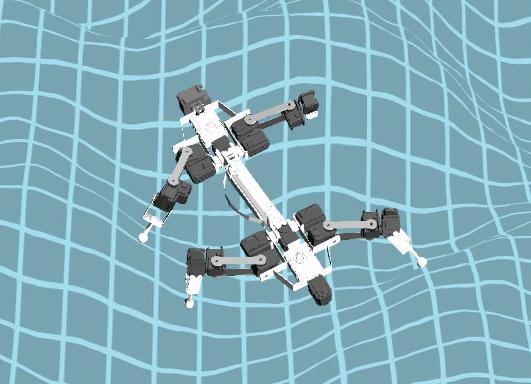
\includegraphics[width=\linewidth]{../img/3/find_tr/krock-bumps.jpg}
    \end{subfigure}
\caption{Krock tries to overcome an obstacle in the \emph{bumps3} map.}
\end{figure}

Due to its characteristic locomotion, Krock tries to overcome the obstacle using the legs to move itself to the top but it fell backs producing a spicky advancement where first it is positive and then negative. The following picture shows the advancemnet on this map with different time windows, $\Delta t$, the greater the smoother.

\begin{figure}[H]
    \centering
    \begin{subfigure}[b]{0.45\textwidth}
        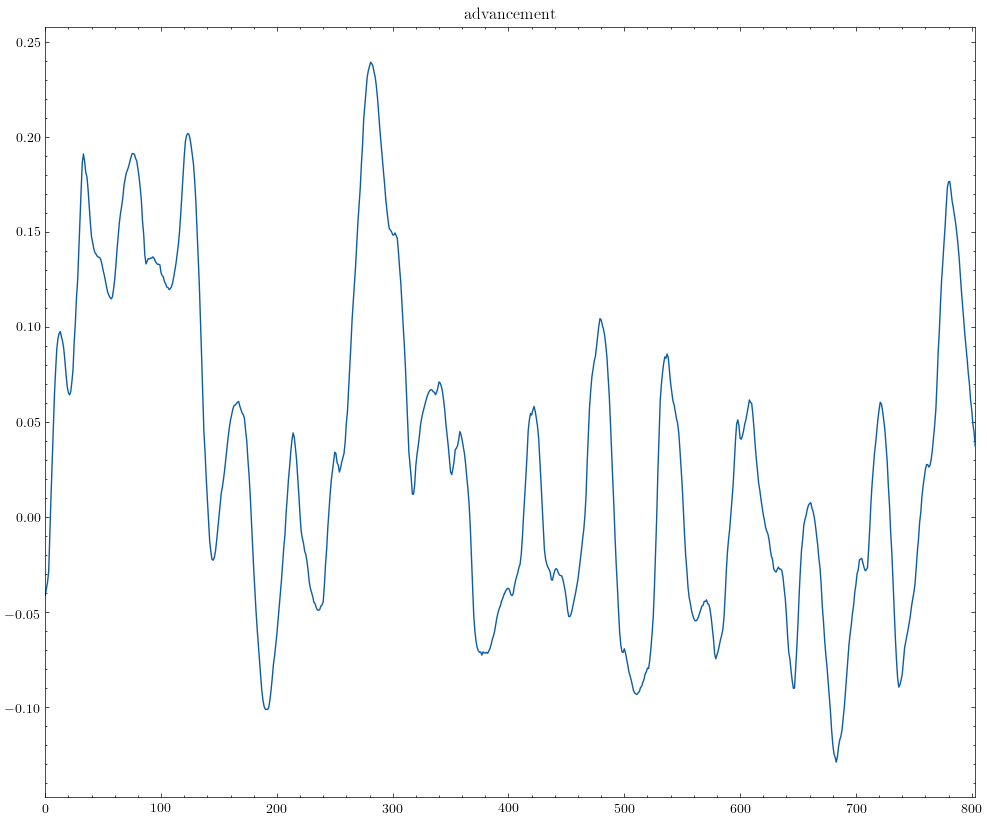
\includegraphics[width=\linewidth]{../img/3/find_tr/100-bumps3}
        \caption{$\Delta t = 2$s.}
    \end{subfigure}

\caption{Advancement over time with different $\Delta t$ on \emph{bumps3}.}
\end{figure}
A wheel robot, on the other hand, will not produce such graph since it cannot free itself easily from an obstacle.

\paragraph{Ramps}
To correctly decide the threshold we must be sure it will not create false negative. For this reason, we check the advancement on the $slope_rocks1$ map with a height scaling factor set to $5$.
\begin{figure}[H]
    \centering
    \begin{subfigure}[b]{0.45\textwidth}
        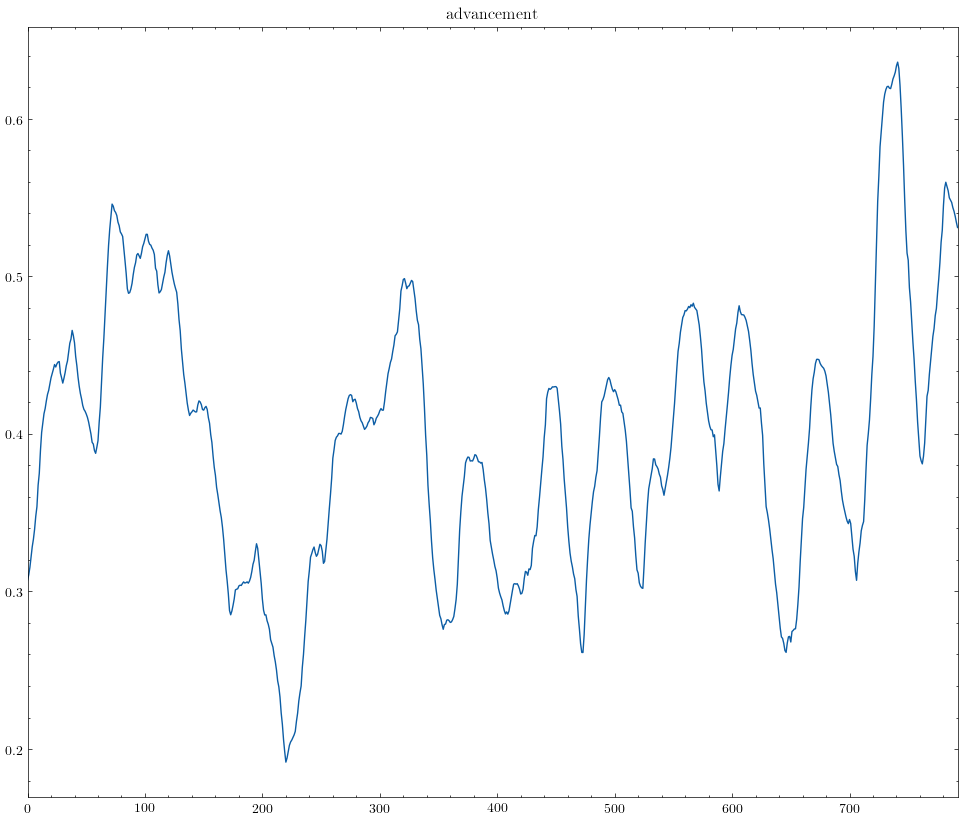
\includegraphics[width=\linewidth]{../img/3/find_tr/100-slope_rocks1}
        \caption{$\Delta t = 2$s.}
    \end{subfigure}
    
    \caption{Advancement over time with different $\Delta t$ on \emph{slope\_rocks3}.}
\end{figure}
We know that those patches are traversable even if sometimes the robot may find it hard to climb them. So, we want to choose a threshold that is beetween the upper bound of \emph{bumps} and beetween the lower bound of \emph{slope\_rocks1}. Thus, good thresholds value is $tr_{\Delta t = 2s} = 20cm$.

\subsection{Estimator}
\label{sec: estimator}
In this section we described the choices behind the evaluated network architecture.
\subsubsection{Vanilla Model}
The original model proposed by Chavez-Garcia et all \cite{omar2018traversability} is a CNN composed by a two $3 \times 3$ convolution layer with $5$ filters; $2 \times 2$ Max-Pooling layer; $3 \times 3$ convolution layer with $5$ filters; a fully connected layer with 128 outputs neurons and a fully connected layers with two neurons. 
\subsubsection{MicroResNet}
We adopt a Residual network, ResNet \cite{he2015deep}, variant. Residual networks are deep convolutional networks consisting of many stacked \" Residual Units \". Intuitively, the residual unit allows the input of a layer to contribute to the next layer's input by being added to the current layer's output. Due to possible different features dimension, the input must go through and identify map to make the addition possible. This allows a stronger gradient flows and mitigates the degradation problem. A \"Residual Units \" is composed by a two $3x3$ \emph{Convolution}, \emph{Batchnorm} \cite{ioffe2015batch} and a \emph{Relu} blocks. Formally defined as: 
\begin{equation}
    \mathbf{y}=\mathcal{F}\left(\mathbf{x},\left\{W_{i}\right\}\right)+h(\mathbf{x})
    \label{eq : resnet}
\end{equation}
Where, $x$ and $y$ are the input and output vector of the layers considered. The function $\mathcal{F}\left(\mathbf{x},\left\{W_{i}\right\}\right)$ is the residual mapping to be learn and $h$ is the identity mapping. The next figure visualises the equation.
\todo[inline]{add resnet image or table}
\begin{figure}[H]
    \centering
    \includegraphics[scale=0.3]{../img/implementation/estimator/resnet_block.png}
    \caption{\emph{Resnet} block \cite{he2015deep}}
\end{figure}
When the input and output shapes mistmatch, the \emph{identity map} is applyed to the input as a $3x3$ Convolution with a stride of 2 to mimic the polling operator. A single block is composed by a $3x3$ \emph{Convolution}, \emph{Batchnorm} and a \emph{Relu} activation function. 
\subsubsection{Preactivation}
Following the recent work of He et al. \cite{he2015identity} we adopt \emph{pre-activation} in each block.\emph{Pre-activation} works by just reversing the order of the operations in a block.

\begin{figure}[H]
    \centering
    \includegraphics[scale=0.2]{../img/implementation/estimator/preactivation.png}
    \caption{\emph{Preactivation} \cite{he2015identity}}
\end{figure}
\subsubsection{Sqeeze and Excitation}
Finally, we also used the \emph{Squeeze and Excitation} (SE) module \cite{hu2017squeeze}. It is a form of attention that weights the channel of each convolutional operation by learnable scaling factors. Formally, for a given transformation, e.g. Convolution, defined as $\bm{F}_{tr}  : \bm{X} \mapsto \bm{U}$, $\bm{X} \in mathbb{R}^{H' \times W' \times C'}$, $\bm{U} \in \mathbb{R}^{H \times W \times C}$, the SE module first squeeze the information by using average pooling, $\bm{F}_{sq}$, the it excitates them using learnable weights, $\bm{F}_{ex}$ and finally, adaptive recalibration is performed, $\bm{F}_{scale}$.
The next figure visualises the SE module.

\begin{figure}[H]
    \centering
    \includegraphics[width=\linewidth]{../img/implementation/estimator/se.png}
    \caption{\emph{Squeeze and Excitation} \cite{hu2017squeeze}}
\end{figure}
\subsubsection{Micro resnet}
Our network is composed by $n$ ResNet blocks, a depth of $d$ and a channel incrementing factor of $2$. Since ResNet assumed an input size of $224\times224$ and perform an aggressive features extraction in the first layer, we called it \emph{head}, as showed in \todo{ref to Resnet Table} we decided to adopt a less aggressive convolution. We tested two kernel sized of $7\times7$ and $3\times3$ with stride of $2$ and $1$ respectively. Lastly, we used LeakyReLU \cite{leakyrelu} with a negative slope of $0.1$ instead of ReLU to allow a better gradient flow during backpropagation. LeakyRelu is defined as follows
\begin{equation}
LeakyRelu(x)=\left\{\begin{array}{ll}{x} & {\text { if } x>0} \\ {0.1 x} & {\text { otherwise }}\end{array}\right.
\end{equation}

We called this model architecture \emph{MicroResNet}. We evaluated $n=[1,2], d=3$ with and without squeeze and excitation and with the two differents \emph{head}'s convolution. All the networks have a starting channel size of $16$. The following table shows the architecture from top to bottom.

\begin{table}[H]
    \centering
    \ra{1.2}
        \begin{tabular}{@{}l|c|c|c|cc@{}}
        \hline
             Input   &  \multicolumn{4}{c}{$(1,78,78)$}  \\ 
            \hline 
            \multirow{12}{*}{Layers} & \multicolumn{2}{c}{$3 \times 3$, $16$ stride $1$} & \multicolumn{2}{c}{$7 \times 7$ $16$ stride $2$} \\
            \cline{2-5}
            &\multicolumn{4}{c}{$2 \times \ 2$ max-pool} \\ 
            \cline{2-5}
            &  \multicolumn{4}{c}{$\begin{bmatrix}
                3  \times 3, & 16 \\
                3  \times  3, & 32 \\  
               \end{bmatrix}$ x 1} \\ 
               \cline{2-5}
               &  SE & - & SE & -\\ 
               \cline{2-5}
               &  \multicolumn{4}{c}{$\begin{bmatrix}
                3  \times 3, & 32 \\
                3  \times  3, & 64 \\  
               \end{bmatrix}$ x 1} \\ 
               \cline{2-5}
               &  SE & - & SE & -\\ 
               \cline{2-5}

               &  \multicolumn{4}{c}{$\begin{bmatrix}
                3  \times 3, & 64 \\
                3  \times  3, & 128 \\  
               \end{bmatrix}$ x 1} \\
               \hline
               &  SE & - & SE & -\\ 
               \cline{2-5}
               &  \multicolumn{4}{c}{average pool, $1$-d fc, softmax} \\ 
               \hline
        
               Parameters &  313,642 & 302,610  &  \textbf{314,282} & 303,250 \\
            \hline
               Size (MB) & 5.93 & 5.71 &  \textbf{2.41} & 2.32 \\ 
               \hline 
        \end{tabular}
        \caption{MicroResNet architecture from top to bottom. Some part of the architecture are equal across models, this is shows by sharing columns in the table.}
    \end{table}
\todo[inline]{this table sucks}
Our models have approximately $35$ times less parameters than the smalles ResNet model, ResNet18, that has $11$M parameters. To simplicity we will use the following notation to describe each architecture variant: \texttt{MicroResNet-{3x3/7x7}-{/SE}}.
\todo[inline]{ask omar help to add margin in the rows}
\todo[inline]{add model picture}

\subsubsection{Normalization}
Before feeding the data to the models, we need to make the patches height invariant to correctly normalize different patches taken from different maps with different height scaling factor. To do so, we subtract the height of the map corresponding \emph{Krock}'s position from the patch to correctly center it. The following figure shows the normalization process on the patch with the square in the middle.
\begin{figure}[H]
    \centering
    \begin{subfigure}[b]{0.32\textwidth}
        \includegraphics[width=\textwidth]{../img/data-aug/2d/square-middle.png}
        \caption{Input}
    \end{subfigure}
    \begin{subfigure}[b]{0.32\textwidth}
        \includegraphics[width=\textwidth]{../img/data-aug/2d/square-middle-center.png}
        \caption{Height centered}
    \end{subfigure}  
    \\
          \begin{subfigure}[b]{0.32\textwidth}
        \includegraphics[width=\textwidth]{../img/data-aug/3d/square-middle.png}
        \caption{Input}
    \end{subfigure}
    \begin{subfigure}[b]{0.32\textwidth}
        \includegraphics[width=\textwidth]{../img/data-aug/3d/square-middle-center.png}
        \caption{Height centered}
    \end{subfigure}  
\caption{Normalization process}
\label{fig: center}
\end{figure}

\subsubsection{Data Augmentation}
\label{sec: data-aug}
Data augmentation is used to change the input of a model in order to produce more training examples. Since our inputs are heightmaps we cannot utilize the classic image manipulations such as shifts, flips, and zooms. Imagine that we have a patch with a wall in front of it, if we random rotate the image the wall may go in a position where the wall is not facing the robot anymore, making the image now traversable with a wrong target. We decided to apply dropout, coarse dropout, and random simplex noise since they are traversability invariant. To illustrate those techniques we are going to use the same square patch showed before \ref{fig: center}.

\paragraph{Dropout} is a technique to randomly set some pixels to zero, in our case we flat some random pixel in the patch. 
\paragraph{Coarse Dropout} similar to dropout, it sets to zero random regions of pixels.
\paragraph{Simplex Noise} is a form of Perlin noise that is mostly used in ground generation. Our idea is to add some noise to make the network generalize better since lots of training maps have only obstacles in flat ground. Since it is computationally expensive, we randomly fist apply the noise to five hundred images with only zeros. Then, we randomly scaled them and add to the input image. 
\begin{figure}[H]
    \centering

        \begin{subfigure}[b]{0.32\textwidth}
            \includegraphics[width=\textwidth]{../img/data-aug/3d/simplex1.png}
            \caption{Features size = 10}
        \end{subfigure}
        \begin{subfigure}[b]{0.32\linewidth}
            \includegraphics[width=\textwidth]{../img/data-aug/3d/simplex2.png}
            \caption{Features size = 20}
            \end{subfigure}    
          \begin{subfigure}[b]{0.32\textwidth}
            \includegraphics[width=\textwidth]{../img/data-aug/3d/simplex3.png}
            \caption{Features size = 30}
        \end{subfigure}    
        \begin{subfigure}[b]{0.32\textwidth}
            \includegraphics[width=\textwidth]{../img/data-aug/3d/simplex4.png}
            \caption{Features size = 40}
        \end{subfigure}    
    \label{fig: simplex-noise}
    \caption{Simplex Noise on flat ground}    
\end{figure}

The following images show the tree data augmentation techniques used applied the input image.
\begin{figure}[H]
    \centering
        \begin{subfigure}[b]{0.32\textwidth}
            \includegraphics[width=\textwidth]{../img/data-aug/2d/center-dropout.png}
            \caption{Dropout}
        \end{subfigure}
        \begin{subfigure}[b]{0.32\linewidth}
            \includegraphics[width=\textwidth]{../img/data-aug/2d/center-coarse-dropout.png}
            \caption{Coarse Dropout}
            \end{subfigure}    

          \begin{subfigure}[b]{0.32\textwidth}
            \includegraphics[width=\textwidth]{../img/data-aug/2d/center-simplex.png}
            \caption{Simplex Noise}

        \end{subfigure}    
        \begin{subfigure}[b]{0.32\textwidth}
            \includegraphics[width=\textwidth]{../img/data-aug/2d/center-aug.png}
            \caption{Final result}
        \end{subfigure}    
    \label{fig: square-patch-aug}
    \caption{Data augmentation applied on a patch.}    
\end{figure}
It follows an other set of figures that shows the data augmentation applyed on different inputs.

\begin{figure}[H]
    \centering
        \begin{subfigure}[b]{0.23\textwidth}
            \includegraphics[width=\textwidth]{../img/data-aug/2d/wall.png}
            \caption{Walls}
        \end{subfigure}
        \begin{subfigure}[b]{0.23\linewidth}
            \includegraphics[width=\textwidth]{../img/data-aug/2d/wall-aug.png}
            \caption{Walls aug}
        \end{subfigure}    
        \begin{subfigure}[b]{0.23\textwidth}
            \includegraphics[width=\textwidth]{../img/data-aug/2d/ramp.png}
            \caption{Ramp}
        \end{subfigure}
        \begin{subfigure}[b]{0.23\linewidth}
            \includegraphics[width=\textwidth]{../img/data-aug/2d/ramp-aug.png}
            \caption{Ramp aug}
        \end{subfigure}    
    \label{fig: others-aug}
    \caption{Data augmentation applyed first on a patch with two walls, then on a ramp.}    
\end{figure}
In all the traning epochs, we data augment each input image $x$ with a probability of $0.8$. Dropout has a probability between $0.05$ and $0.1$. Coarse dropout with a probability of $0.02$ and $0.1$ with a size of the lower resolution image from which to sample the dropout between $0.6$ and $0.8$. Simplex noise with a feature size between $1$ and $50$ with a random scaling factor between $6$ and $10$. 
\end{document}